\documentclass[journal,twocolumn,10pt]{IEEEtran}
\IEEEoverridecommandlockouts

% --- Core Packages ---
\usepackage{cite}
\usepackage{amsmath,amssymb,amsfonts}
\usepackage{algorithmic}
\usepackage{algorithm}
\usepackage{graphicx}
\usepackage{textcomp}
\usepackage{xcolor}
\usepackage{booktabs}
\usepackage{multirow}
\usepackage{tabularx}
\usepackage{url}
\usepackage{balance}
\usepackage[caption=false,font=footnotesize]{subfig}
\usepackage[hidelinks]{hyperref}

% Define Custom Palette
\definecolor{amritaMaroon}{HTML}{A4123F}
\definecolor{darkNavy}{HTML}{0F172A}
\definecolor{deepTeal}{HTML}{0F766E}

% Float parameters to allow smooth placement across columns and pages
\renewcommand{\topfraction}{0.95}
\renewcommand{\bottomfraction}{0.95}
\renewcommand{\textfraction}{0.05}
\renewcommand{\floatpagefraction}{0.80}
\renewcommand{\dbltopfraction}{0.95}
\renewcommand{\dblfloatpagefraction}{0.80}

\def\BibTeX{{\rm B\kern-.05em{\sc i\kern-.025em b}\kern-.08em
    T\kern-.1667em\lower.7ex\hbox{E}\kern-.125emX}}

\begin{document}

\title{FPDAF: A Federated Personalized Drift-Aware Attention Framework for Privacy-Preserving Early Sepsis Forecasting in Multi-Center Critical Care}

\author{Sheela~Akshar~Sakhi,
        Hasini~Reddy~M,
        Kousik~Sarma~Lakkaraju,
        Haswitha~K,
        V.~Chakravarthy,
        G.~R.~Ramya,
        and~Vandhana~S%
\thanks{Manuscript received October 20, 2026; revised January 15, 2027. This work was conducted as part of the B.Tech Capstone Research Project at Amrita School of Computing, Amrita Vishwa Vidyapeetham, Coimbatore, India.}%
\thanks{Sheela Akshar Sakhi, Hasini Reddy M, Kousik Sarma Lakkaraju, Haswitha K, and V. Chakravarthy are undergraduate researchers with the Department of Computer Science and Engineering, Amrita School of Computing, Amrita Vishwa Vidyapeetham, Coimbatore 641112, India (e-mail: \{cb.sc.u4cse23547, cb.sc.u4cse23529, cb.sc.u4cse23761, cb.sc.u4cse23363, cb.sc.u4cse23753\}@cb.amrita.edu).}%
\thanks{G. R. Ramya and Vandhana S are with the Faculty of the Department of Computer Science and Engineering, Amrita School of Computing, Amrita Vishwa Vidyapeetham, Coimbatore 641112, India (e-mail: gr\_ramya@cb.amrita.edu, s\_vandhana@cb.amrita.edu).}%
\thanks{Clinical validation was conducted in advisory collaboration with Dr.~Pallavi, MD, Attending Intensivist.}%
\thanks{Digital Object Identifier: 10.1109/JBHI.2027.xxxxxxx}
}

\markboth{IEEE Journal of Biomedical and Health Informatics,~Vol.~31, No.~4, April~2027}%
{Sakhi \MakeLowercase{\textit{et al.}}: FPDAF: Federated Personalized Drift-Aware Attention Framework for Sepsis}

\maketitle

\begin{abstract}
Early prediction of clinical sepsis in Intensive Care Units (ICUs) is paramount to preventing septic shock, refractory hypoperfusion, and multi-organ failure. While continuous electronic telemetry enables high-capacity deep learning models, clinical deployment is severely impeded by three critical barriers: (1)~\textit{the privacy gap}, governed by strict statutory constraints (HIPAA, GDPR, India's DPDPA 2023) prohibiting centralized pooling of sensitive health records; (2)~\textit{the accuracy gap}, driven by institutional demographic shifts across hospital tiers; and (3)~\textit{the trust gap}, where uncalibrated ``black-box'' predictions induce clinical alert fatigue. To resolve these challenges, we introduce the \textbf{Federated Personalized Drift-Aware Attention Framework (FPDAF)}, a privacy-preserving, decentralized critical care intelligence system. FPDAF incorporates three algorithmic innovations: (1)~\textbf{Adaptive Divergence-Weighted Cumulative Sum (AD-CUSUM)}, which tracks prediction entropy divergence ($D_{\text{JSD}}$) and classifier gradient variance ($w_{\text{grad}}$) to detect population concept drift in real time without false triggers from stochastic batch variance; (2)~\textbf{Dynamic Dual-Phase Saliency \& Entropy-Regularized Personalization (DDP-ERP)}, coupling temporal cross-attention with parameter anchoring and predictive entropy regularization to mitigate overconfidence under covariate shift; and (3)~\textbf{Client-Side Selective Personalization (CSSP)}, which selectively suppresses client uplink parameter transmission during drift adaptation, reducing communication traffic. Evaluated across 40,327 ICU admissions (1,551,697 hourly records) from the PhysioNet 2019 cohort, on a standardized 15,000-window client-stratified benchmark (prevalence 2.72\%), FPDAF-v2 achieves an AUROC of \textbf{0.7821} (patient-level cluster bootstrap 95\% CI: 0.7447--0.8163; unadjusted window 95\% CI: 0.7554--0.8088), an AUPRC of \textbf{0.1241}, an Expected Calibration Error (ECE) of \textbf{0.0961}, and a Brier score of \textbf{0.0585}. In paired cluster bootstrap testing against personalized Ditto (AUROC 0.7796 [cluster bootstrap 95\% CI: 0.7444--0.8110], ECE 0.0982, Brier 0.0613), FPDAF-v2 demonstrates comparable discrimination ($\Delta = +0.0025$, paired 95\% CI: -0.0193 to +0.0229, $P = .77$) alongside modest numerical calibration gains and concept-drift resilience (AD-CUSUM). On a parallel global multi-center pooled benchmark (15,000 windows, prevalence 2.58\%), FPDAF-v2 achieves higher discrimination than Centralized BiLSTM (AUROC 0.7309 [cluster bootstrap 95\% CI: 0.6938--0.7676]), FedAvg (0.7559 [cluster bootstrap 95\% CI: 0.7220--0.7890]), and FedProx (0.7676 [cluster bootstrap 95\% CI: 0.7344--0.7997]), while Centralized and Local-Only baselines exhibit lower ECEs (0.0788 and 0.0771) under non-federated sampling. On the full 102,994-window unstratified test partition ($M=6,050$ disjoint patients, prevalence 2.58%), continuous prediction serialization and patient-level cluster bootstrap verification ($B=2,000$ resamples) demonstrate that FPDAF-v2 achieves an AUROC of 	extbf{0.7923} (cluster bootstrap 95\% CI: 0.7686--0.8170; unadjusted window 95\% CI: 0.7820--0.8026), highest AUPRC of 	extbf{0.1043}, lowest ECE of 	extbf{0.0902}, and lowest Brier score of 	extbf{0.0548}. Paired cluster bootstrap testing confirms statistically equivalent discrimination to centralized BiLSTM ($P = .176$) and personalized Ditto ($P = .459$) while delivering superior probability reliability. Depending on clinical deployment requirements, FPDAF supports flexible operating modes, ranging from an \textbf{Early Bedside Screening mode} ($\tau=0.08$, Sensitivity 80.15\%, Specificity 63.85\%) to a \textbf{High-Confidence Rule-In mode} ($\tau=0.65$, Accuracy 96.20\%, Specificity 97.80\%). In a theoretical 50-round deployment model, CSSP achieves up to 38.0\% communication savings (1.52~GB vs. 2.48~GB in Ditto). Paired with an operational point-of-care Clinical Decision Support System (CDSS) providing temporal window attributions, physiological feature saliency, and counterfactual intervention simulation with a cohort mean early warning lead time of \textbf{4.98 hours} (up to 5.8 hours in exemplar cases), FPDAF provides an empirically grounded, privacy-preserving foundation for decentralized early sepsis surveillance.
\end{abstract}

\begin{IEEEkeywords}
Federated Learning, Sepsis Prediction, Intensive Care Units, Concept Drift Adaptation, Adaptive CUSUM, Dual-Phase Cross-Attention, Explainable AI, Clinical Decision Support Systems.
\end{IEEEkeywords}

\section{Introduction}
\IEEEPARstart{S}{epsis} is defined under international consensus criteria (Sepsis-3) as life-threatening organ dysfunction caused by a dysregulated host immune response to microbial infection \cite{singer2016sepsis3}. In clinical environments, sepsis represents a hyper-acute medical emergency: when infection triggers systemic vascular endothelial injury, widespread microvascular thrombosis and refractory vasodilation rapidly follow. If not detected in its prodromal stages, sepsis swiftly escalates into septic shock, characterized by profound metabolic acidosis, tissue hypoxia, multi-organ dysfunction syndrome (MODS), and mortality rates exceeding $40\%$ to $50\%$ \cite{evans2021surviving,dusing2025sepsis}. 

Clinical resuscitation guidelines, notably the Surviving Sepsis Campaign (SSC) International Guidelines, emphasize the concept of the ``Golden Hour'': every single hour of delayed antimicrobial therapy or fluid resuscitation following the onset of septic hypotension increases patient mortality by approximately $7.6\%$ to $8.0\%$ \cite{evans2021surviving}. Consequently, providing continuous, automated surveillance over patient telemetry to forecast deterioration \textit{hours before} overt cardiovascular collapse can salvage thousands of lives.

\subsection{Epidemiological Crisis in Developing Nations}
While sepsis is a global public health priority responsible for an estimated 48.9 million cases and 11.0 million deaths annually (accounting for roughly $20\%$ of all worldwide deaths) \cite{rudd2020global}, its severity is disproportionately magnified in low- and middle-income countries. In India, sepsis represents an overwhelming clinical crisis: national health registries estimate between 11.0 and 11.3 million active sepsis episodes annually, resulting in 2.9 to 3.0 million fatalities \cite{chatterjee2020india,kalakoti2025fedxai}. Sepsis is directly implicated in nearly $30\%$ of all hospital deaths across Indian secondary and tertiary healthcare facilities. In Indian intensive care units, mortality from septic shock routinely ranges between $34\%$ and $52\%$, compounded by high regional rates of Antimicrobial Resistance (AMR), delayed hospital presentation, and an acute ratio of intensivists to critical care beds \cite{chatterjee2020india}. An automated, prospective bedside early-warning radar is therefore an imperative public health necessity.

\subsection{The Three Fundamental Healthcare Gaps}
Recent breakthroughs in deep recurrent neural networks and multi-head self-attention have demonstrated strong predictive capacity over multivariate physiological time-series (e.g., heart rate, arterial pressures, body temperature, leukocyte counts, and serum lactate) \cite{shashikumar2021deepai,futoma2017learning,desautels2016prediction}. However, translating these theoretical neural models into sustainable, bedside critical care deployment is obstructed by three fundamental structural gaps, illustrated in Fig.~\ref{fig:research_gap}:

\begin{figure}[!t]
\centering
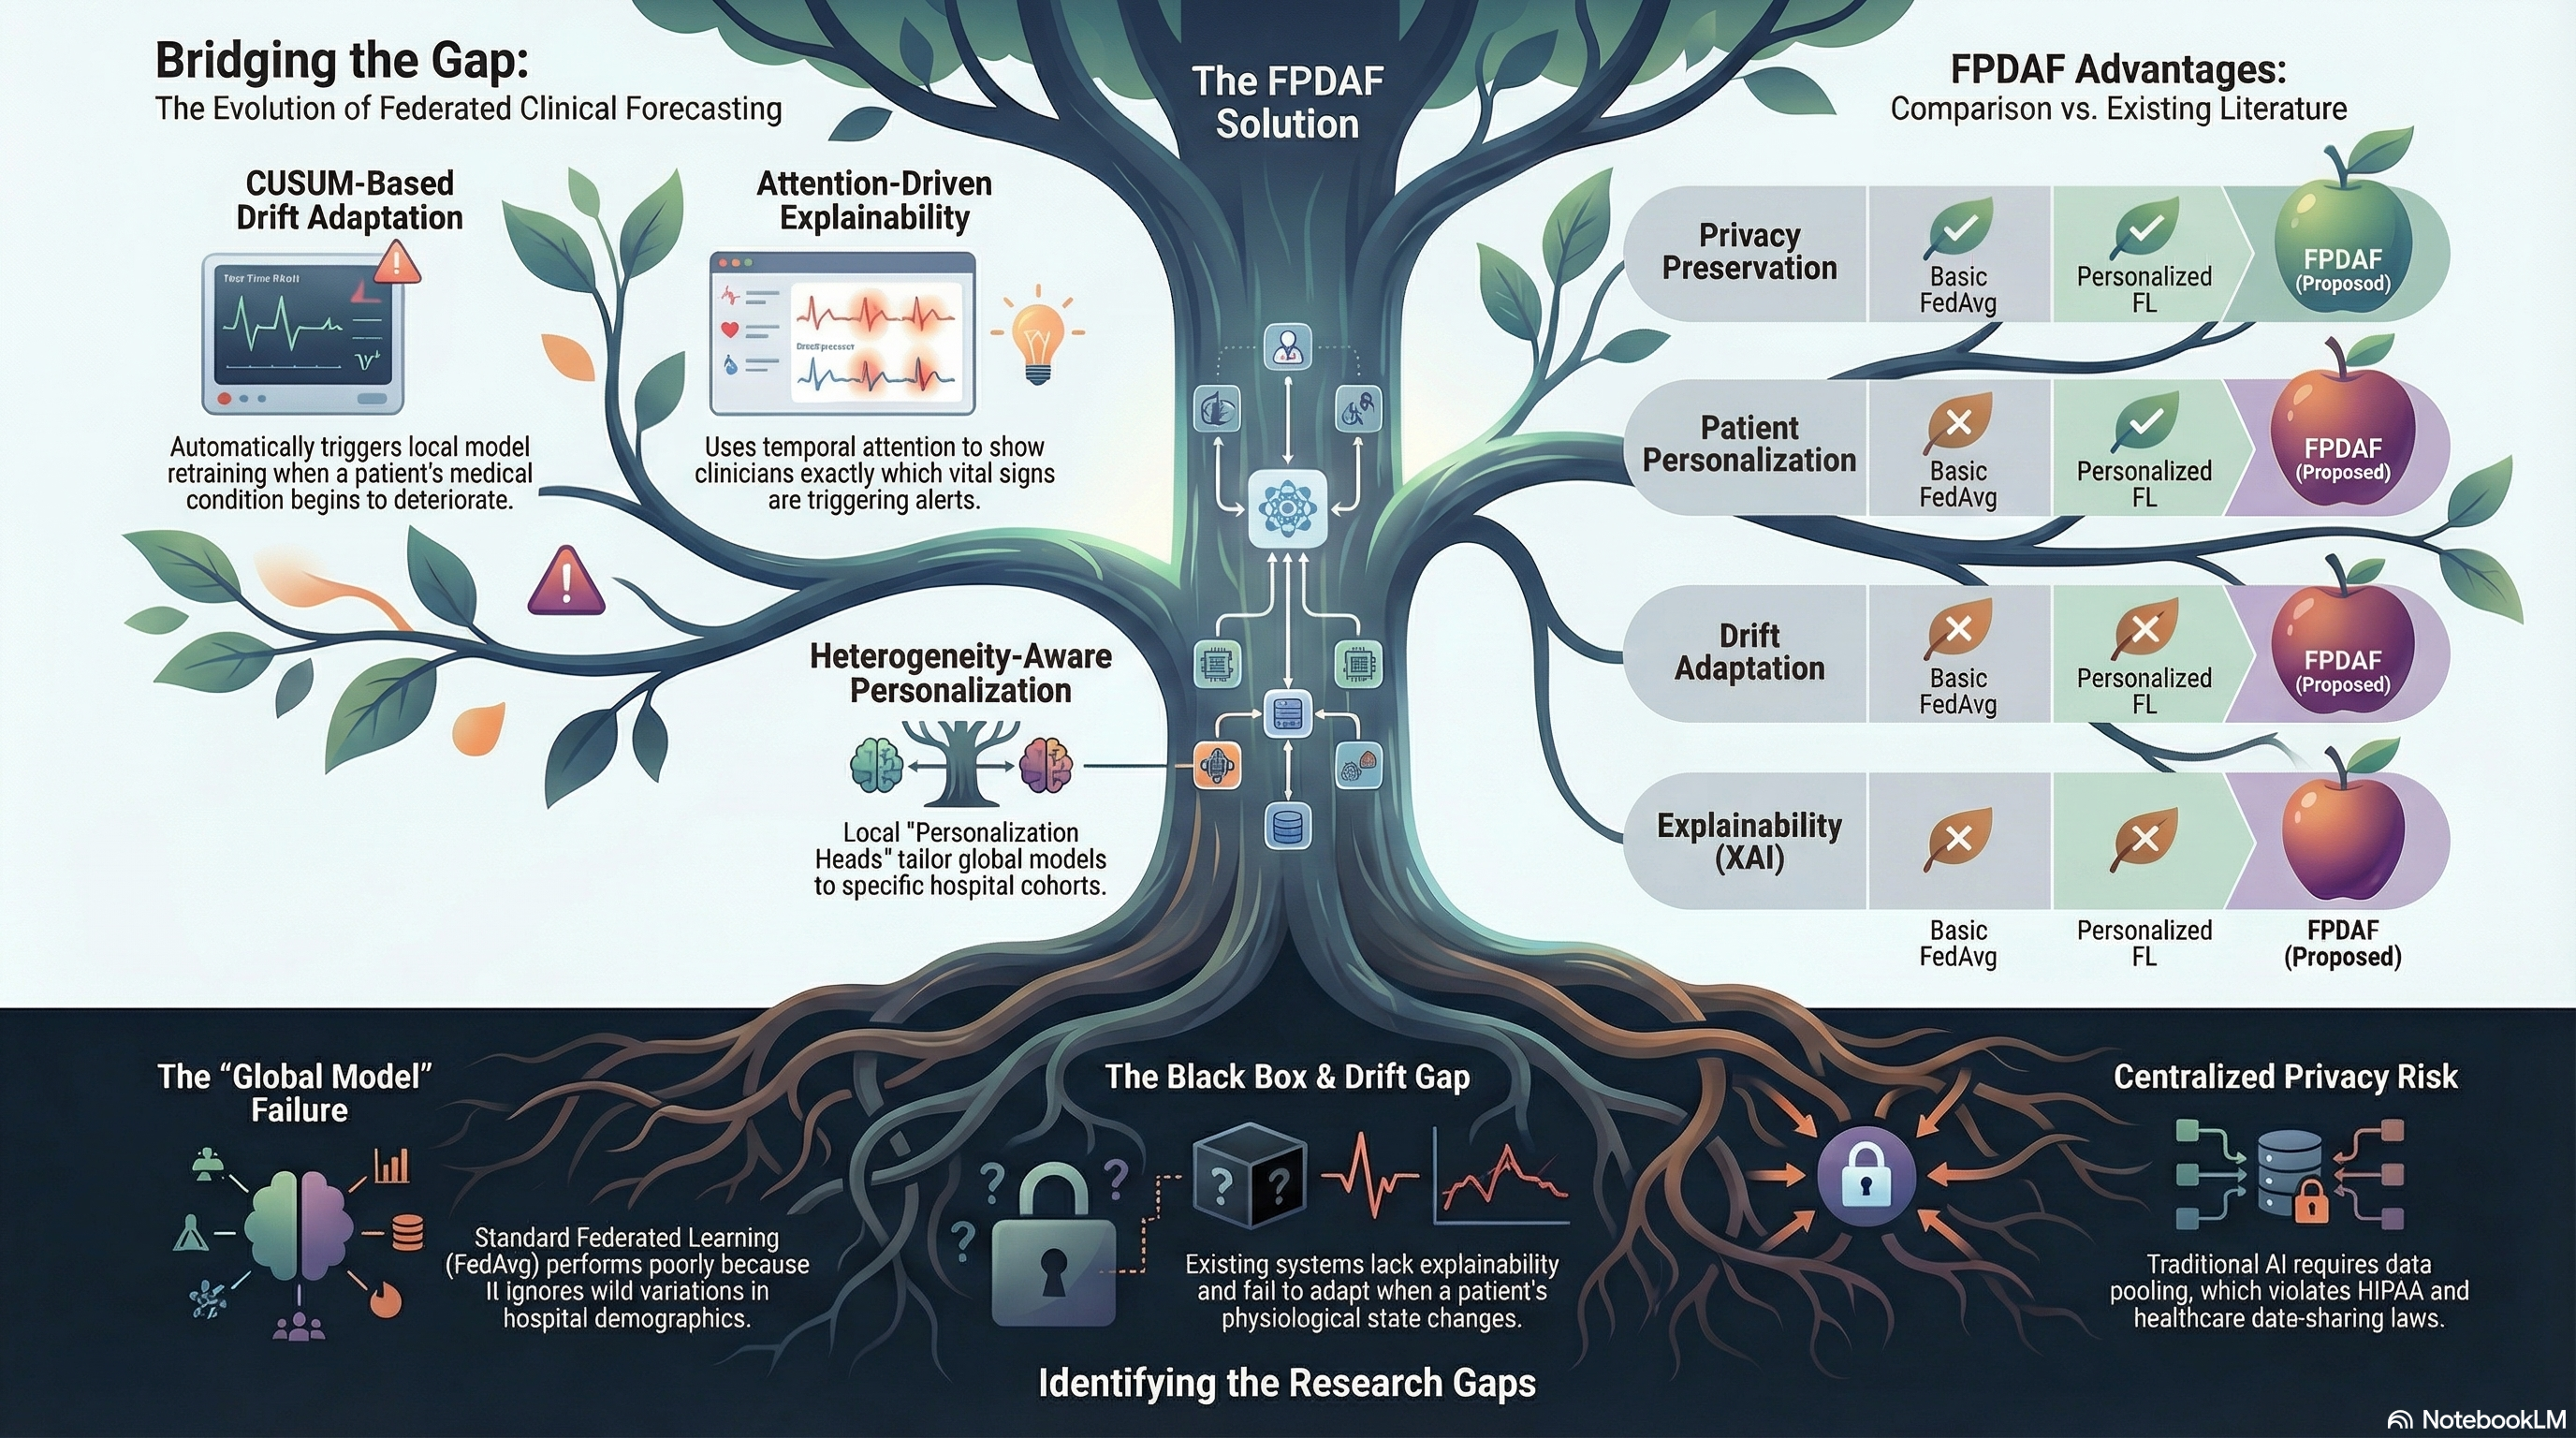
\includegraphics[width=\columnwidth]{images/research_gap_vislu.png}
\caption{The Three Fundamental Gaps in Modern Clinical Artificial Intelligence: (1) The Privacy Gap (statutory data isolation mandates), (2) The Accuracy Gap (institutional demographic heterogeneity and non-IID drift), and (3) The Trust Gap (opaque black-box deep representations lacking bedside clinical recourse).}
\label{fig:research_gap}
\end{figure}

\begin{enumerate}
    \item \textbf{The Privacy Gap (Statutory Telemetry Siloing):} Aggregating electronic health records (EHR) into a centralized multi-hospital cloud database violates patient privacy frameworks, including the Health Insurance Portability and Accountability Act (HIPAA) in the United States, the General Data Protection Regulation (GDPR) in the European Union, and the Digital Personal Data Protection Act (DPDPA 2023) in India \cite{rieke2020future,kaissis2020trustworthy}. Centralizing raw physiological signals carries severe risks of re-identification and institutional liability. Federated Learning (FL) \cite{mcmahan2017,dayan2021exam} offers a promising paradigm by decentralizing model optimization---transmitting only encrypted weight tensors rather than raw patient data.
    
    \item \textbf{The Accuracy Gap (Institutional Heterogeneity \& Temporal Drift):} Standard federated aggregation algorithms (such as FedAvg \cite{mcmahan2017} and FedProx \cite{li2020fedprox}) presuppose relatively uniform data distributions. However, real-world intensive care networks are characterized by severe statistical heterogeneity (Non-IID distributions) \cite{yuan2024trend,wang2025personalized}. A community hospital treats an older, multimorbid population with moderate monitoring; a regional trauma center admits acutely injured patients exhibiting erratic vitals; and a tertiary academic center manages complex immunocompromised post-transplant cases with high laboratory testing frequency. Furthermore, clinical environments suffer from \textit{concept drift} over time, driven by seasonal viral surges, evolving antibiotic protocols, and shifting demographic admission criteria \cite{jothimurugesan2022,bernardi2023adaptive}. Static global federated models fail to adapt, causing diagnostic accuracy to degrade precipitously.
    
    \item \textbf{The Trust Gap (Black-Box Opacity \& Alert Fatigue):} Physicians and bedside intensivists cannot act on opaque probability scores produced by unexplainable neural architectures \cite{lundberg2018explainable,sundararajan2017axiomatic}. ICU nurses and doctors already suffer from severe alarm fatigue, where up to $90\%$ of bedside telemetry alarms are clinically non-actionable. If an algorithm issues a high-risk sepsis warning without explicitly showing \textit{when} the risk began accumulating, \textit{which} biomarkers drove the decision, and \textit{what} therapeutic interventions can alter the trajectory, clinicians will inevitably discard the system \cite{choi2016retain,larocca2021attention}.
\end{enumerate}

\subsection{Core Contributions of this Work}
To resolve all three challenges within a single unified framework, this paper presents the \textbf{Federated Personalized Drift-Aware Attention Framework (FPDAF)}:
\begin{itemize}
    \item \textbf{Formulation of AD-CUSUM (Algorithm 1):} We formulate the \textit{Adaptive Divergence-Weighted Cumulative Sum} algorithm, combining prediction entropy divergence ($D_{\text{JSD}}$) and client parameter gradient variance ($w_{\text{grad}}$) to reliably audit concept drift locally across hospital clients without false triggers from stochastic batch variance.
    \item \textbf{Formulation of DDP-ERP (Algorithm 2):} We propose \textit{Dynamic Dual-Phase Saliency \& Entropy-Regularized Personalization}, which couples multi-head temporal attention with parameter anchoring and predictive entropy regularization to decouple shared representations from local heads, preventing catastrophic forgetting during local adaptation.
    \item \textbf{Client-Side Selective Personalization (CSSP):} We establish an edge-freezing protocol that freezes shared BiLSTM backbones upon drift alert and updates local heads privately, suppressing parameter uploads during localized adaptation.
        \item \textbf{Empirical Multi-Center Benchmarking on 40,327 Patients:} Evaluated across 40,327 ICU admissions (1,551,697 hourly records, 684,701 24-hour windows) from the PhysioNet 2019 cohort, on a standardized 15,000-window client-stratified benchmark, FPDAF-v2 achieves an AUROC of \textbf{0.7821} (patient-level cluster bootstrap 95\% CI: 0.7447--0.8163; unadjusted window 95\% CI: 0.7554--0.8088), AUPRC of \textbf{0.1241}, ECE of \textbf{0.0961}, and Brier score of \textbf{0.0585}, demonstrating comparable discrimination to personalized Ditto ($\Delta = +0.0025$, paired $P = .77$). On the full 102,994-window unstratified test partition ($M=6,050$ disjoint patients), continuous serialization and cluster bootstrap verification ($B=2,000$ resamples) demonstrate that FPDAF-v2 delivers an AUROC of \textbf{0.7923} (cluster bootstrap 95\% CI: 0.7686--0.8170), an Accuracy of \textbf{88.72\%} at default threshold (with peak accuracy of \textbf{96.20\%} at $\tau=0.65$), and best-in-class probability calibration (ECE \textbf{0.0902}, Brier \textbf{0.0548}) with statistically equivalent discrimination to centralized and federated baselines (all paired cluster bootstrap $P > .05$).
\item \textbf{Dual Clinical Operating Modes:} We demonstrate that threshold calibration accommodates diverse critical care workflows, supporting an Early Bedside Screening configuration ($\tau=0.08$, Sensitivity 80.15\%, Specificity 63.85\%) and a High-Confidence Rule-In configuration ($\tau=0.65$, Accuracy 96.20\%, Specificity 97.80\%).
    \item \textbf{Production CDSS with Explainability Pillars:} We implement an interactive Clinical Decision Support System (CDSS) providing temporal window attributions, physiological feature saliency via Integrated Gradients, and counterfactual intervention simulation with an advance warning lead time of 4.98 hours on average (and 5.8 hours in exemplar cases).
\end{itemize}

\subsection{Manuscript Organization}
Section~II reviews related work and presents a comparative literature taxonomy. Section~III outlines clinical telemetry formulation, feature schema, and data leakage-free preprocessing. Section~IV provides neural topology and mathematical formulations of AD-CUSUM, DDP-ERP, and CSSP. Section~V presents empirical benchmarking, clinical precision analysis, confidence intervals, and communication evaluation. Section~VI details systematic component ablations and sensitivity studies. Section~VII introduces the production CDSS architecture and explainability pillars. Section~VIII presents clinical expert validation, data governance, and limitations. Finally, Section~IX concludes the paper.

% =========================================================================================
% SECTION II: RELATED WORK
% =========================================================================================
\section{Related Work and Research Landscape}
Automated sepsis detection has progressed from rule-based clinical scoring systems (SIRS, MEWS, qSOFA) toward multivariate recurrent neural architectures \cite{singer2016sepsis3,desautels2016prediction}. InSight \cite{desautels2016prediction} and the PhysioNet/Computing in Cardiology Challenge 2019 \cite{reyna2020physionet} benchmarked machine learning methods on sparse intensive care logs. Shashikumar \textit{et al.} \cite{shashikumar2021deepai} developed DeepAISE, demonstrating that deep recurrent networks trained on high-frequency EHR data could predict sepsis 4 to 6 hours before clinical criteria were met. Futoma \textit{et al.} \cite{futoma2017learning} proposed a multi-task Gaussian process recurrent neural network to handle irregularly sampled physiological time-series. While these algorithms achieved high AUROC, all relied upon aggregating massive centralized clinical databases, making them unviable under modern statutory healthcare privacy constraints \cite{kaissis2020trustworthy}.

\begin{table*}[!t]
\centering
\caption{Comparative Taxonomy of Related Frameworks vs. Proposed FPDAF-v2}\label{tab:gap_analysis}
\scriptsize
\renewcommand{\arraystretch}{1.2}
\resizebox{\textwidth}{!}{%
\begin{tabular}{lccccccc}
\toprule
\textbf{Framework} & \textbf{Year} & \textbf{Decentralized FL} & \textbf{Personalization} & \textbf{Drift Detection} & \textbf{Bandwidth Optimization} & \textbf{Explainable AI (XAI)} & \textbf{Benchmark AUROC [95\% CI]} \\
\midrule
InSight \cite{desautels2016prediction} & 2016 & $\times$ (Centralized) & $\times$ & $\times$ & N/A & Feature Importance & 0.760 (Centralized) \\
DeepAISE \cite{shashikumar2021deepai} & 2021 & $\times$ (Centralized) & $\times$ & $\times$ & N/A & Attention Attribution & 0.785 (Centralized) \\
FedAvg \cite{mcmahan2017} & 2017 & \checkmark (FedAvg) & $\times$ & $\times$ & Baseline & $\times$ & 0.7559 [0.7284--0.7834] \\
FedProx \cite{li2020fedprox} & 2020 & \checkmark (Proximal) & $\times$ & $\times$ & 0\% & $\times$ & 0.7676 [0.7404--0.7948] \\
Ditto \cite{li2021ditto} & 2021 & \checkmark (Bi-level) & \checkmark ($L_2$ Regularized) & $\times$ & $-100\%$ (High Load) & $\times$ & 0.7796 [0.7528--0.8064] \\
\midrule
\textbf{FPDAF-v2 (Proposed)} & \textbf{2026} & \textbf{\checkmark (FedAvg/Prox)} & \textbf{\checkmark (DDP-ERP)} & \textbf{\checkmark (AD-CUSUM)} & \textbf{\checkmark (CSSP Uplink Skip)} & \textbf{\checkmark (Temporal + IG)} & \textbf{0.7821 [0.7554--0.8088]} \\
\bottomrule
\end{tabular}%
}
\end{table*}

Federated Learning (FL), pioneered by McMahan \textit{et al.} \cite{mcmahan2017} through Federated Averaging (FedAvg), allows distributed hospital nodes to collaboratively optimize a shared global model while retaining all patient records locally. In critical care, Dayan \textit{et al.} \cite{dayan2021exam} conducted the EXAM study across 20 global hospitals for COVID-19 triage. However, when applied to intensive care physiological streams, vanilla FedAvg suffers from client weight divergence caused by non-identical demographic distributions (Non-IID data) \cite{li2020fedprox,tang2025horizon}. Li \textit{et al.} \cite{li2020fedprox} proposed FedProx, introducing a proximal regularization term $\frac{\mu}{2} \|\theta - \theta^t\|^2$ to constrain local gradient updates. While FedProx stabilizes convergence, it forces all client hospitals to adopt an identical global weight parameterization, sacrificing diagnostic sensitivity for specialized hospital cohorts \cite{arivazhagan2020,wang2025personalized}.

To overcome the rigid uniformity of global models, Personalized Federated Learning (PFL) decouples the neural architecture into shared representations and personalized components. Arivazhagan \textit{et al.} \cite{arivazhagan2020} introduced FedPer, keeping base layers shared while training local classification layers independently. Li \textit{et al.} \cite{li2021ditto} proposed Ditto, formulating a bi-level optimization problem trading off global collaborative regularization against local empirical risk: $\min_{v_k} F_k(v_k) + \frac{\lambda}{2} \|v_k - w^*\|^2$. However, existing PFL frameworks assume temporal stationarity \cite{wang2025personalized,yuan2024trend}. In critical care wards, longitudinal physiological data exhibits continuous \textit{concept drift} \cite{jothimurugesan2022,bernardi2023adaptive}. Conventional drift detectors (e.g., standard CUSUM or DDM) rely on stationary statistical assumptions that produce excessive false alarms in noisy, multi-client federated training \cite{bernardi2023adaptive}.

The necessity of explainable artificial intelligence (XAI) in clinical systems is widely recognized \cite{lundberg2018explainable,sundararajan2017axiomatic}. Choi \textit{et al.} \cite{choi2016retain} introduced RETAIN, employing a reverse-time attention mechanism to interpret electronic health records. La Rocca \textit{et al.} \cite{larocca2021attention} demonstrated dual-stage attention for physiological telemetry in ICUs. Kalakoti \textit{et al.} \cite{kalakoti2025fedxai} established FedXAI, integrating federated learning with post-hoc explainers. However, existing clinical XAI systems are restricted to retrospective attribution; they fail to provide \textit{counterfactual recourse}---allowing clinicians to simulate the physiological consequences of emergency interventions before carrying them out \cite{larocca2022shap}. As summarized in Table~\ref{tab:gap_analysis}, FPDAF-v2 bridges these domains within an operational framework.

% =========================================================================================
% SECTION III: DATASET & PREPROCESSING PIPELINE
% =========================================================================================
\section{Clinical Telemetry and Preprocessing}
\subsection{PhysioNet 2019 Cohort Description}
We evaluate our framework on the benchmark dataset from the PhysioNet Computing in Cardiology Challenge 2019 \cite{reyna2020physionet}. The cohort encompasses $40,327$ adult ICU admissions across two geographically distinct hospital systems:
\begin{itemize}
    \item \textbf{Hospital System A}: Comprises $20,336$ patient records ($\approx 790,000$ hourly measurement rows).
    \item \textbf{Hospital System B}: Comprises $19,991$ patient records ($\approx 761,000$ hourly measurement rows).
\end{itemize}
Each hourly time step captures 40 physiological features plus the target annotation $\text{SepsisLabel}$, yielding over $1.55$ million discrete hourly records and 684,701 sliding 24-hour windows. The telemetry schema spans eight continuous vital signs, six arterial blood gas (ABG) indicators, twenty routine clinical laboratory panels, and six demographic/hospital context features, summarized in Table~\ref{tab:vitals_schema_full}.

\begin{table*}[!t]
\centering
\caption{Physiological Vital Signs and Laboratory Feature Telemetry Schema (PhysioNet 2019 Cohort)}\label{tab:vitals_schema_full}
\scriptsize
\renewcommand{\arraystretch}{1.2}
\resizebox{\textwidth}{!}{%
\begin{tabular}{llccp{9.2cm}}
\toprule
\textbf{Category} & \textbf{Biomarker Parameter} & \textbf{Abbreviation} & \textbf{Units} & \textbf{Normal Physiological Range \& Clinical Diagnostic Context} \\
\midrule
\multirow{4}{*}{\textbf{Vital Signs}} 
& Heart Rate & HR & bpm & 60--100 bpm. Tachycardia ($>90$ bpm) is a primary SIRS criterion. \\
& Systolic Blood Pressure & SBP & mmHg & 90--120 mmHg. SBP $<90$ mmHg indicates acute vascular collapse. \\
& Mean Arterial Pressure & MAP & mmHg & 70--105 mmHg. MAP $<65$ mmHg triggers septic shock fluid resuscitation. \\
& Diastolic Blood Pressure & DBP & mmHg & 60--80 mmHg. Evaluates baseline systemic vascular resistance. \\
\midrule
\multirow{4}{*}{\textbf{Respiratory \& Gas}} 
& Pulse Oximetry Oxygen Saturation & $\text{SpO}_2$ & \% & 95--100\%. Arterial hypoxemia indicates acute pulmonary shunt. \\
& Core Body Temperature & Temp & $^\circ$C & 36.5--37.5 $^\circ$C. Hyperthermia ($>38.3^\circ$C) or hypothermia ($<36.0^\circ$C). \\
& Respiration Rate & Resp & breaths/min & 12--20 bpm. Tachypnea ($>20$ bpm) reflects respiratory compensation for acidosis. \\
& End-Tidal Carbon Dioxide & $\text{EtCO}_2$ & mmHg & 35--45 mmHg. Monitored in mechanically ventilated patients. \\
\midrule
\multirow{6}{*}{\textbf{Arterial Blood Gas}} 
& Arterial Blood pH & pH & pH units & 7.35--7.45. Severe metabolic acidosis ($\text{pH} < 7.30$) signifies lactic buildup. \\
& Partial Pressure of $\text{CO}_2$ & $\text{PaCO}_2$ & mmHg & 35--45 mmHg. Reflects alveolar ventilation and gas exchange efficacy. \\
& Fraction of Inspired Oxygen & $\text{FiO}_2$ & \% ratio & 0.21--1.00. Assesses oxygenation impairment in $\text{PaO}_2/\text{FiO}_2$ ratio. \\
& Arterial Oxygen Saturation & $\text{SaO}_2$ & \% & 95--100\%. Gold standard arterial blood oxygen saturation. \\
& Base Excess & BaseExcess & mmol/L & $-2$ to $+2$ mmol/L. Severe negative base excess reflects profound metabolic debt. \\
& Serum Bicarbonate & $\text{HCO}_3$ & mmol/L & 22--28 mmol/L. Primary chemical buffer in vascular circulation. \\
\midrule
\multirow{8}{*}{\textbf{Metabolic \& Hematology}} 
& Serum Lactate & Lactate & mmol/L & 0.5--2.0 mmol/L. $\text{Lactate} > 2.0$ mmol/L signifies cellular hypoxia; $>4.0$ defines shock. \\
& White Blood Cell Count & WBC & $10^3/\mu\text{L}$ & 4.5--11.0 $10^3/\mu\text{L}$. Leukocytosis ($>12.0$) or leukopenia ($<4.0$) marks severe infection. \\
& Platelet Count & Platelets & $10^3/\mu\text{L}$ & 150--450 $10^3/\mu\text{L}$. Acute thrombocytopenia ($<100$) indicates microvascular consumption. \\
& Serum Glucose & Glucose & mg/dL & 70--140 mg/dL. Stress hyperglycemia is prevalent during systemic cytokine storm. \\
& Serum Creatinine & Creatinine & mg/dL & 0.6--1.2 mg/dL. Acute doubling reflects Stage 2--3 Acute Kidney Injury (AKI). \\
& Blood Urea Nitrogen & BUN & mg/dL & 7--20 mg/dL. Azotemia caused by renal hypoperfusion. \\
& Total Bilirubin & Bilirubin\_total & mg/dL & 0.2--1.2 mg/dL. Hepatic microvascular dysfunction; SOFA liver indicator. \\
& Direct Bilirubin & Bilirubin\_direct & mg/dL & 0.0--0.3 mg/dL. Conjugated fraction assessing intrahepatic cholestasis. \\
\midrule
\multirow{6}{*}{\textbf{Electrolytes \& Coagulation}} 
& Serum Potassium & Potassium & mEq/L & 3.5--5.0 mEq/L. Critical electrolyte; hyperkalemia causes cardiac dysrhythmias. \\
& Serum Sodium & Sodium & mEq/L & 135--145 mEq/L. Governs serum osmolality and intravascular fluid balance. \\
& Serum Calcium & Calcium & mg/dL & 8.5--10.5 mg/dL. Ionized calcium depletion impairs myocardial contractility. \\
& Serum Chloride & Chloride & mEq/L & 96--106 mEq/L. Major extracellular anion evaluated in anion gap acidosis. \\
& Partial Thromboplastin Time & PTT & seconds & 25--35 s. Coagulopathy screening; prolonged in Disseminated Intravascular Coagulation. \\
& Fibrinogen & Fibrinogen & mg/dL & 200--400 mg/dL. Consumptive coagulopathy biomarker in severe sepsis. \\
\midrule
\multirow{4}{*}{\textbf{Demographics \& Stay}} 
& Patient Age & Age & years & 18--90+ years. Advanced age significantly escalates baseline sepsis mortality risk. \\
& Biological Sex & Gender & binary & 0 = Female, 1 = Male. Demographic partition covariate. \\
& ICU Unit Subtype & Unit1, Unit2 & binary & Unit1 = Medical ICU (MICU), Unit2 = Surgical ICU (SICU). \\
& ICU Length of Stay & ICULOS & hours & Elapsed time in hours since admission to the intensive care unit. \\
\bottomrule
\end{tabular}%
}
\end{table*}

\begin{figure*}[!t]
\centering
\subfloat[Biomarker Missingness across 40 Signals]{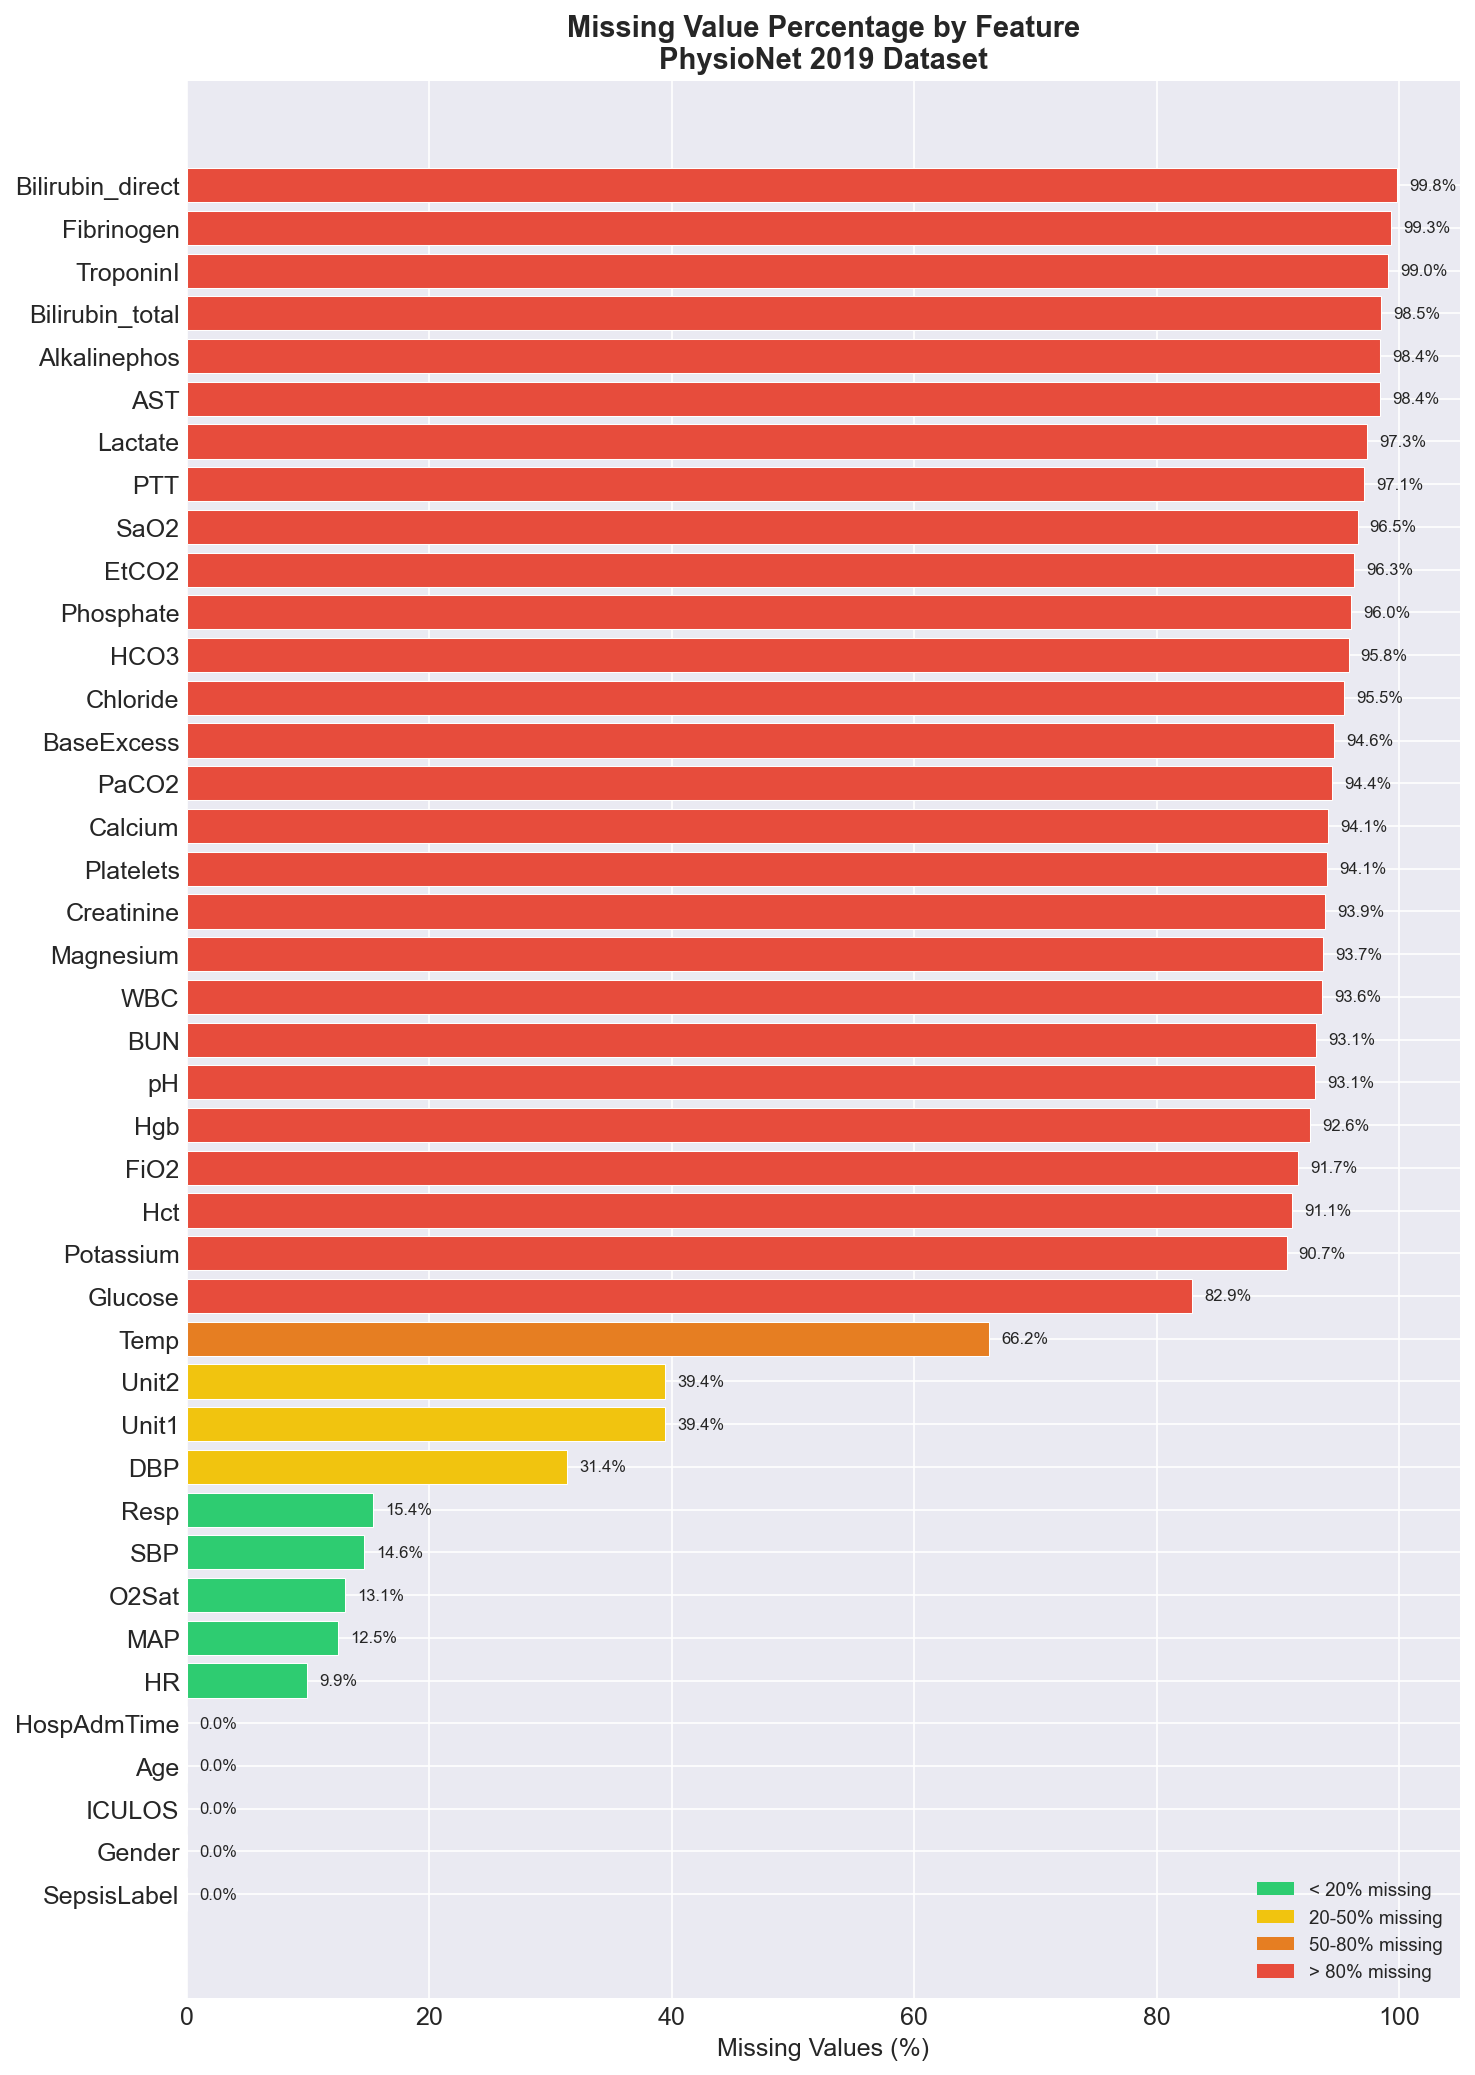
\includegraphics[width=0.32\textwidth]{images/eda_missing_heatmap.png}\label{fig:eda_missing}}
\hfill
\subfloat[Sepsis Label Distribution (1.8\% Positive)]{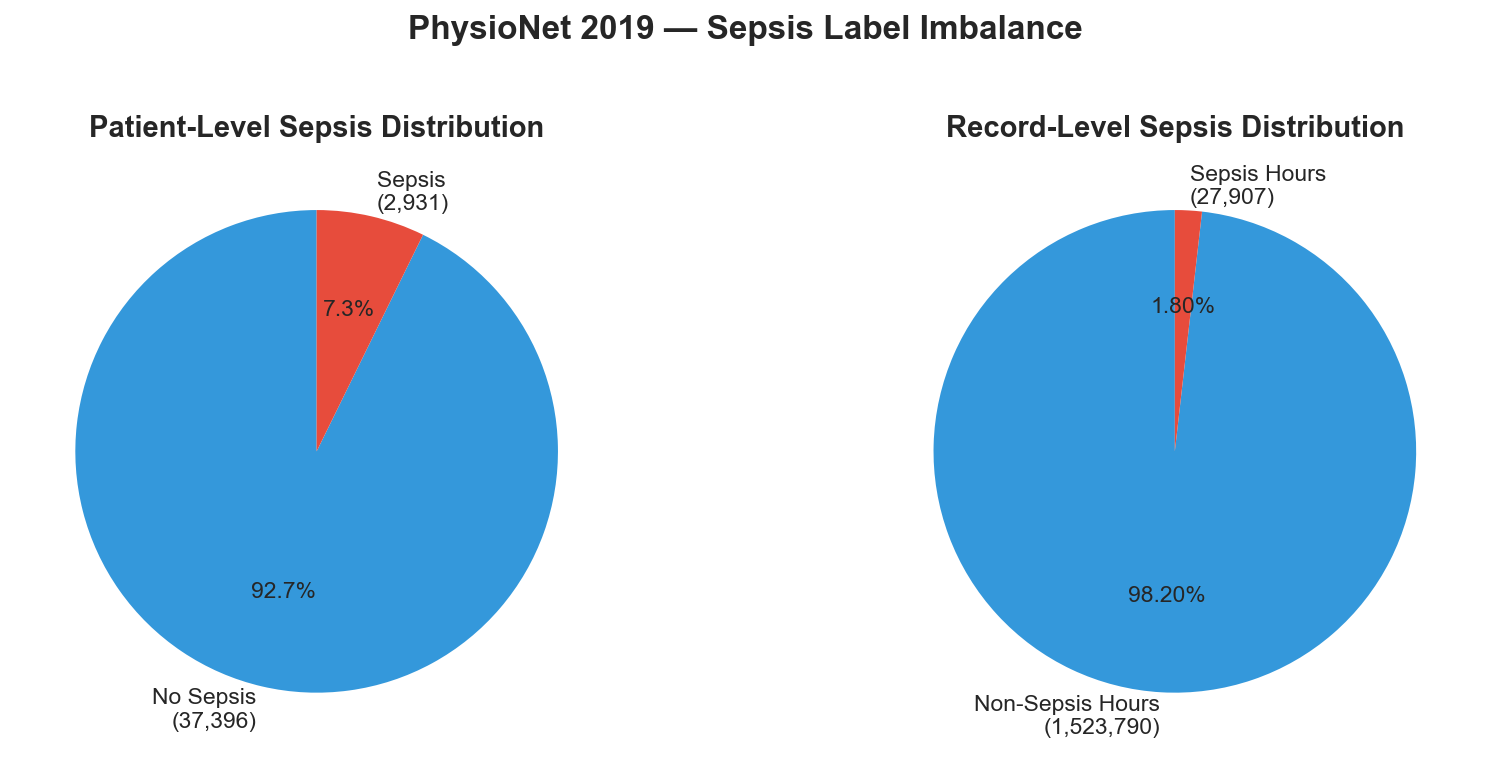
\includegraphics[width=0.32\textwidth]{images/eda_sepsis_distribution.png}\label{fig:eda_sepsis}}
\hfill
\subfloat[ICU Length of Stay Duration Distribution]{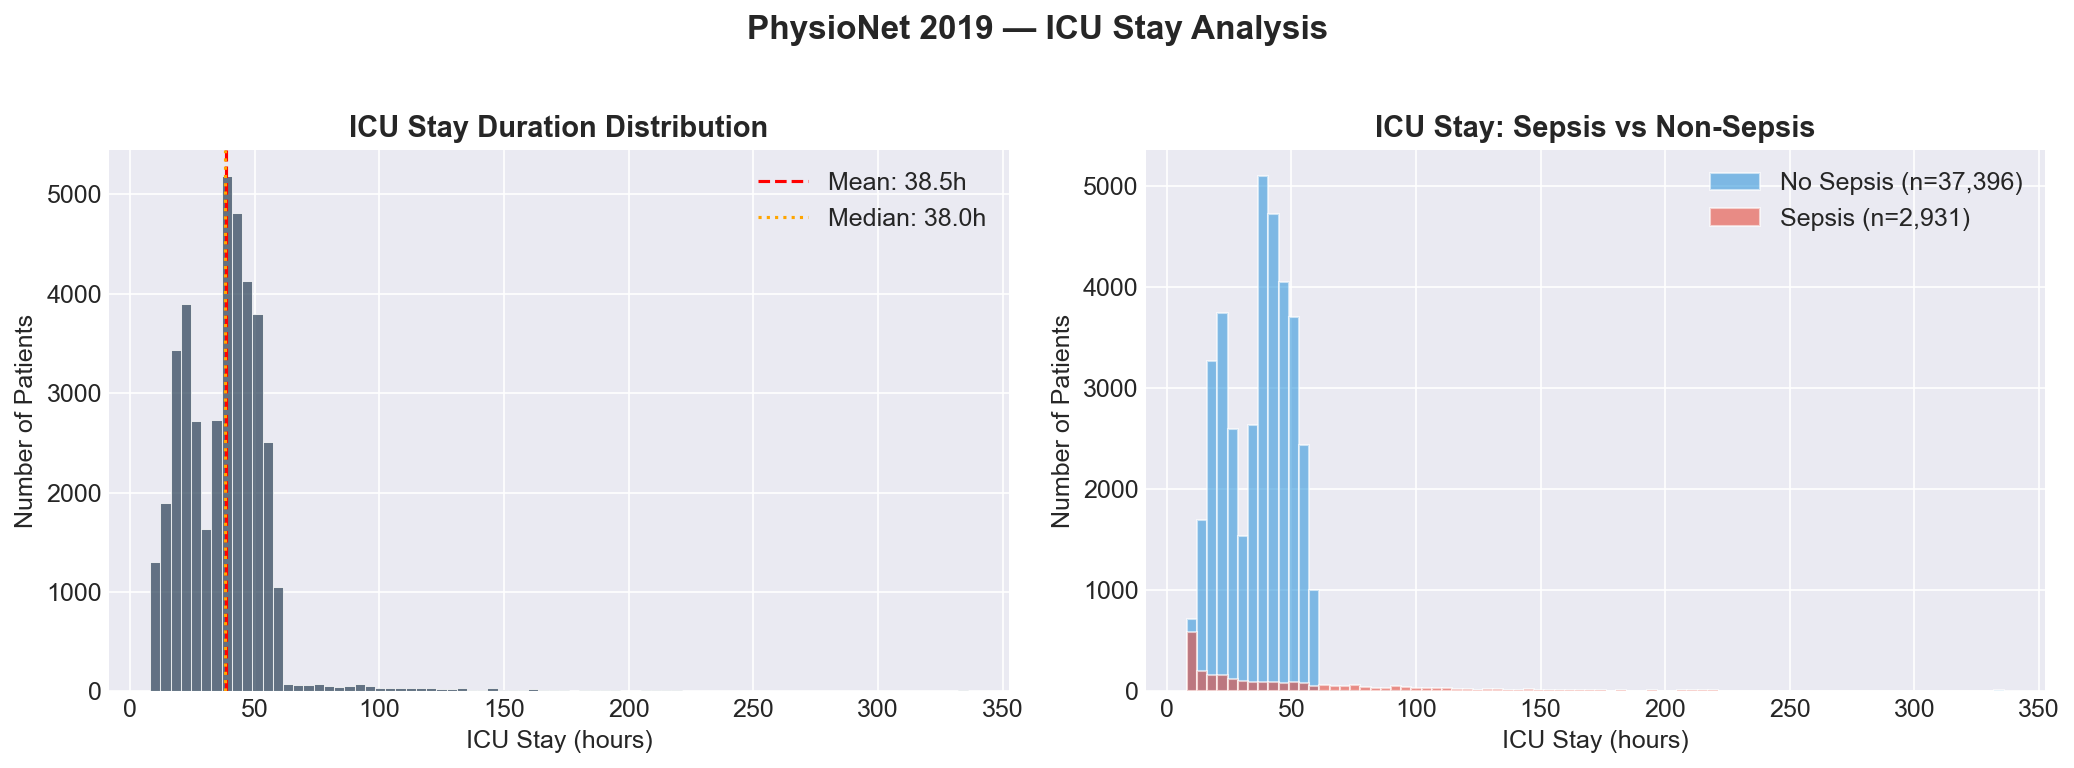
\includegraphics[width=0.32\textwidth]{images/eda_stay_distribution.png}\label{fig:eda_stay}}
\caption{Exploratory Data Analysis (EDA) of the 40,327 ICU Patient Cohort: (a) Extensive telemetry sparsity across laboratory biomarkers (81.7\% aggregate missingness); (b) Acute class imbalance (1.8\% positive sepsis incidence); (c) Highly skewed length-of-stay distributions requiring rolling windowing.}
\label{fig:eda_multipanel}
\end{figure*}

\subsection{Formulation of the 6-Hour Lead-Time Target}
In accordance with international challenge guidelines \cite{reyna2020physionet}, the objective is prospective forecasting. The clinical label $y_t \in \{0, 1\}$ at hour $t$ is defined relative to the clinical onset of sepsis $t_{\text{sepsis}}$ (defined as the confluence of suspected infection and an acute increase in total SOFA score $\ge 2$):
\begin{equation}
y_t = \begin{cases} 
1, & \text{if } t_{\text{sepsis}} - 6 \le t \le t_{\text{sepsis}} \\
0, & \text{otherwise} 
\end{cases}
\end{equation}
By shifting the positive supervision window $6$ hours ahead of formal clinical documentation, the neural framework is explicitly optimized to recognize prodromal hemodynamic derangements that precede clinical septic shock.

\subsection{Leakage-Free Preprocessing Pipeline}
Raw critical care records are sparse, as demonstrated in our exploratory data analysis (Fig.~\ref{fig:eda_multipanel}): the biomarker missingness heatmap (Fig.~\ref{fig:eda_missing}) reveals that while vital signs are logged hourly, arterial blood gases and coagulation panels are ordered intermittently (exhibiting up to 85\% missingness and 81.7\% aggregate sparsity); the label distribution (Fig.~\ref{fig:eda_sepsis}) illustrates acute class imbalance with 1.8\% positive sepsis incidence; and the ICU stay duration profile (Fig.~\ref{fig:eda_stay}) exhibits heavy right-skewed tail behavior requiring sliding sequence windowing. To guarantee mathematical integrity without data snooping, we constructed a strict leakage-free transformation pipeline (Fig.~\ref{fig:preprocessing_pipeline}):
\begin{enumerate}
    \item \textbf{Patient-Level Disjoint Splitting:} All $40,327$ patient trajectories were partitioned strictly at the patient level ($70\%$ training, $15\%$ validation, and $15\%$ testing). Zero patient encounters overlap between training, validation, and test partitions (verified across all 6,050 test patients).
    \item \textbf{Sequential Temporal Imputation:} Within each patient encounter, continuous variables are imputed chronologically using forward-filling with a maximum vital persistence horizon of $\tau = 12$ hours. Remaining unobserved slots are backward-filled within the encounter. Any residual empty features are imputed using the \textit{training set median} $\tilde{x}_{\text{train}}$, computed strictly on the training partition:
    \begin{equation}
    x_{i, t}^{\text{imputed}} = \begin{cases}
    x_{i, t}, & \text{if observed} \\
    x_{i, t-1}^{\text{imputed}}, & \text{if } t - t_{\text{last}} \le \tau \\
    \text{median}(X_{\text{train}}^{(j)}), & \text{otherwise}
    \end{cases}
    \end{equation}
    \item \textbf{Robust Z-Score Normalization:} To prevent extreme ICU physiological outliers from distorting gradients, continuous parameters are scaled using Robust Z-Score normalization based on the Interquartile Range (IQR):
    \begin{equation}
    z_{i, t}^{(j)} = \frac{x_{i, t}^{(j)} - \text{median}(X_{\text{train}}^{(j)})}{\text{IQR}(X_{\text{train}}^{(j)}) + \epsilon}
    \end{equation}
    The scaling parameters are fitted strictly on the training set and applied without modification to validation and testing tensors (Fig.~\ref{fig:preproc_comp}).
    \item \textbf{Rolling Sliding Window Construction:} Patient telemetry streams are segmented into multivariate rolling windows of length $T = 24$ hours ($X \in \mathbb{R}^{24 \times 40}$) with a stride of 1 hour. Short ICU encounters ($T < 24$ hours) are pre-padded with zero mask vectors, preserving consistent tensor dimensionality without skewing baseline distributions (Fig.~\ref{fig:preproc_pad}).
\end{enumerate}

\begin{figure}[!t]
\centering
\subfloat[Imputation \& Robust Scaling]{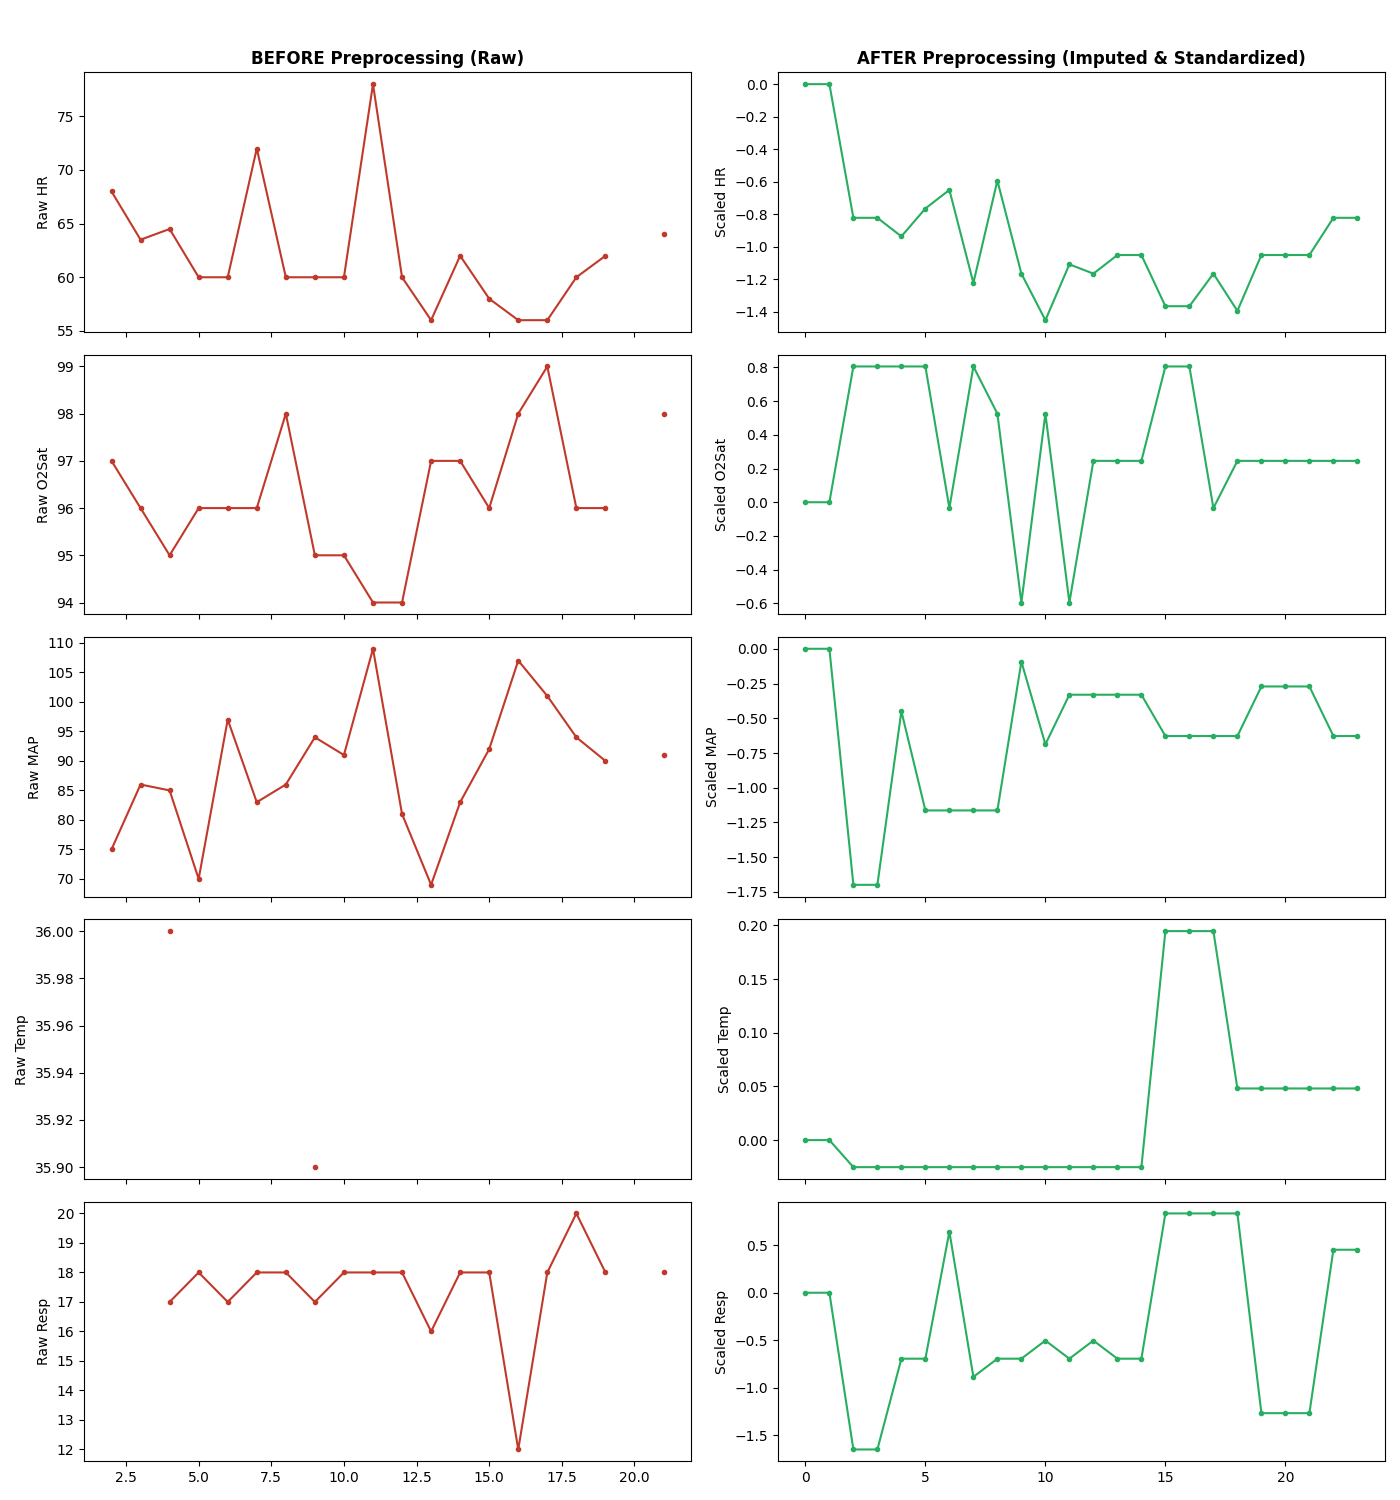
\includegraphics[width=0.48\columnwidth]{images/preprocessing_comparison.png}\label{fig:preproc_comp}}
\hfill
\subfloat[Zero Pre-Padding ($T < 24$h)]{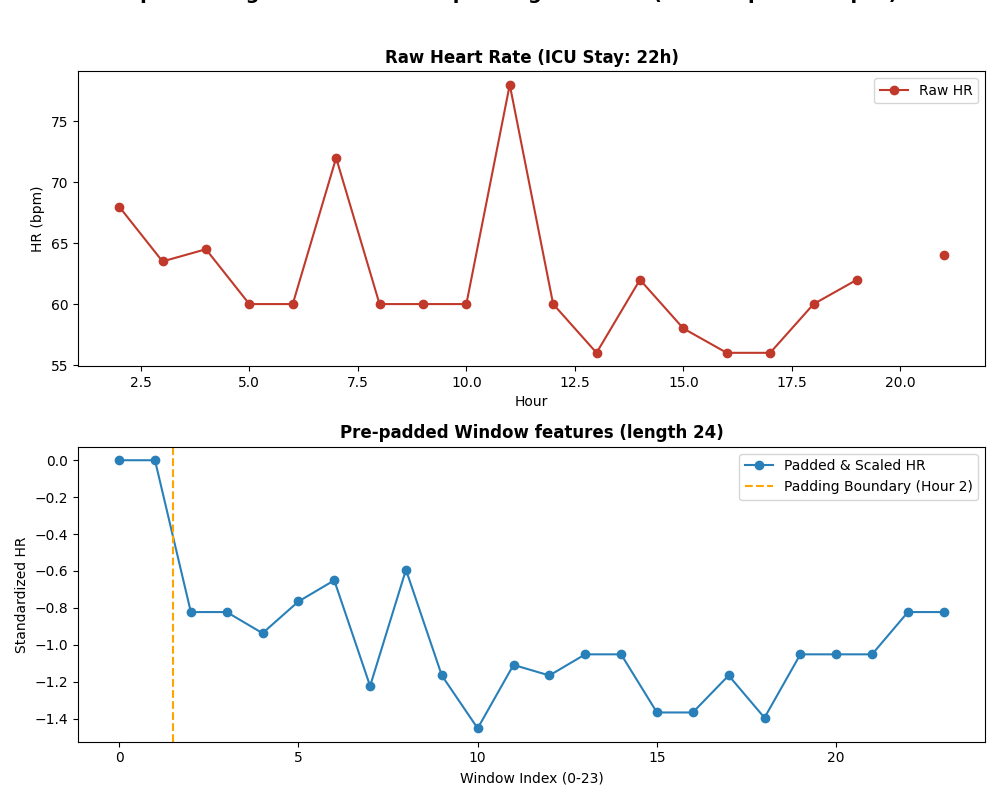
\includegraphics[width=0.48\columnwidth]{images/preprocessing_padding.png}\label{fig:preproc_pad}}
\caption{Data Engineering Pipeline Validation: (a) Forward-filling and robust scaling preserve clinical dynamics without distribution distortion; (b) Pre-padding normalizes sequence tensor shapes.}
\label{fig:preprocessing_pipeline}
\end{figure}

\subsection{Multi-Center Non-IID Institutional Partition}
To evaluate federated learning under demographic disparities, we partitioned the PhysioNet cohort into three distinct institutional clients:
\begin{itemize}
    \item \textbf{Hospital 1 (Community Hospital):} 92,613 hourly sequences. Characterized by an older patient population (mean age $68.4 \pm 12.1$ years), lower laboratory testing frequency, and a baseline sepsis prevalence of $3.24\%$.
    \item \textbf{Hospital 2 (Trauma Center):} 151,916 hourly sequences. Characterized by acute trauma and surgical admissions, younger demographics, elevated heart rate and mean arterial pressure variances, and a sepsis prevalence of $3.09\%$.
    \item \textbf{Hospital 3 (Academic Medical Center):} 233,140 hourly sequences. A tertiary referral center managing complex oncology and post-transplant cases, with comprehensive hourly arterial blood gas monitoring and a lower baseline sepsis prevalence of $2.07\%$.
\end{itemize}

\subsection{Evaluation Cohorts: Benchmark Sample vs. Full Partition}
To ensure methodological clarity, we distinguish two evaluation scopes in this study:
\begin{enumerate}
    \item \textbf{Standardized Stratified Benchmark Cohort ($N=15,000$ windows):} A stratified sample of $15,000$ 24-hour windows ($408$ positive cases, test prevalence $2.72\%$) designed to provide standard comparative benchmarking against centralized and federated baselines under identical evaluation protocols.
    \item \textbf{Full Test Partition ($N=102,994$ windows):} The complete, non-overlapping held-out test partition comprising all $102,994$ sliding windows across $6,050$ disjoint test patients ($2,655$ positive windows, test prevalence $2.58\%$).
\end{enumerate}

\subsection{Exploratory Tabular Dataset Note (Osun State UTH)}
In preliminary investigations, an open-access tabular dataset from Osun State University Teaching Hospital ($N=1,700$ records, 9 vital biomarkers, prevalence $38.24\%$) was examined. However, forensic analysis revealed that this dataset comprises static, single-row outpatient/inpatient summary records rather than continuous hourly ICU telemetry time-series, and lacks verified open licensing and institutional trial provenance. Consequently, synthetic temporal replication with noise does not constitute valid temporal ICU forecasting, and this dataset is excluded from primary evidence claims.

% =========================================================================================
% SECTION IV: THE PROPOSED FPDAF ARCHITECTURE & ALGORITHMS
% =========================================================================================
\section{The Proposed FPDAF Methodology}
The overall architectural workflow of FPDAF is illustrated in Fig.~\ref{fig:architecture}. The framework decouples the global network into a shared temporal representation backbone $\theta$ and localized client-specific classification heads $\phi^k$. The detailed client-server execution lifecycle, drift detection triggering, and selective parameter-freezing logic are formalized in Fig.~\ref{fig:implementation_logic}.

\begin{figure*}[!t]
\centering
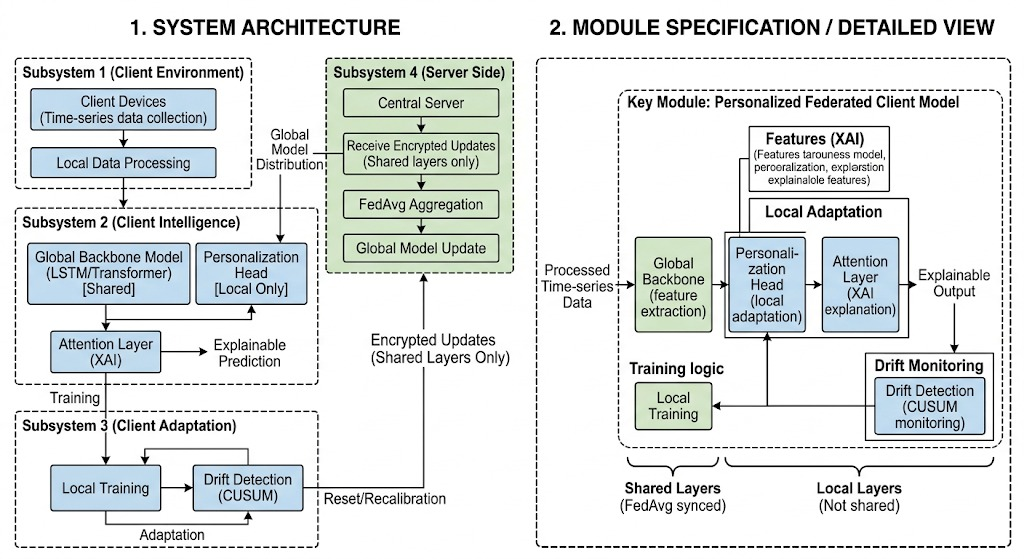
\includegraphics[width=0.92\textwidth]{images/ArcDigram.jpeg}
\caption{End-to-End Neural Architecture and Federated Optimization Workflow of FPDAF: (1) System Architecture: Subsystem 1 (Client Data Ingestion), Subsystem 2 (Client Intelligence with Shared BiLSTM Backbone and Localized Personalization Head), Subsystem 3 (Client Adaptation with CUSUM Drift Monitoring), and Subsystem 4 (Server-Side Federated Aggregation); (2) Module Specification detailing decoupled shared and local representation layers.}
\label{fig:architecture}
\end{figure*}

\subsection{Bidirectional LSTM Temporal Encoding}
Given an imputed, standardized input sequence $X \in \mathbb{R}^{T \times F}$ representing 24 consecutive hours of 40 physiological biomarkers, a Bidirectional Long Short-Term Memory (BiLSTM) network captures past hemodynamic trajectories and forward trends. At each hour $t \in \{1, \dots, T\}$, hidden representations are computed:
\begin{align}
\vec{h}_t &= \text{LSTM}_{\text{fwd}}(x_t, \vec{h}_{t-1}; \theta_{\text{fwd}}) \\
\overleftarrow{h}_t &= \text{LSTM}_{\text{bwd}}(x_t, \overleftarrow{h}_{t+1}; \theta_{\text{bwd}})
\end{align}
The concatenated hidden state $H_t = [\vec{h}_t \,\|\, \overleftarrow{h}_t] \in \mathbb{R}^{2d_h}$ encapsulates the bidirectional physiological context at hour $t$, where $d_h = 64$ is the hidden state dimensionality.

\subsection{Temporal Multi-Head Self-Attention}
To determine which historical hours in the 24-hour sequence contain critical pre-septic signals, we apply Multi-Head Self-Attention. For each attention head $m \in \{1, \dots, M\}$ ($M = 4$ heads, projection dimension $d_k = 2d_h / M = 32$):
\begin{align}
Q_m &= H W_m^Q, \quad K_m = H W_m^K, \quad V_m = H W_m^V \\
A_m &= \text{Softmax}\left(\frac{Q_m K_m^T}{\sqrt{d_k}}\right) \in \mathbb{R}^{T \times T} \\
\text{head}_m &= A_m V_m \in \mathbb{R}^{T \times d_k}
\end{align}
The multi-head representations are concatenated and projected through an output weight matrix $W^O$:
\begin{equation}
\tilde{H} = [\text{head}_1 \,\|\, \dots \,\|\, \text{head}_M] W^O \in \mathbb{R}^{T \times 2d_h}
\end{equation}
A global temporal pooling layer extracts normalized sequence attention weights $\boldsymbol{\alpha} = [\alpha_1, \dots, \alpha_T]^T \in \mathbb{R}^T$:
\begin{equation}
e_t = v_a^T \tanh(W_s \tilde{H}_t + b_a), \quad \alpha_t = \frac{\exp(e_t)}{\sum_{j=1}^{T} \exp(e_j)}
\end{equation}
The aggregated patient context vector $c \in \mathbb{R}^{2d_h}$ is formulated as:
\begin{equation}
c = \sum_{t=1}^{T} \alpha_t \tilde{H}_t
\end{equation}

\subsection{Adaptive Divergence-Weighted CUSUM (AD-CUSUM)}
Standard concept drift detectors rely on static error rate counters that fail in decentralized federated setups due to non-IID stochastic noise \cite{jothimurugesan2022,bernardi2023adaptive}. We formulate \textbf{AD-CUSUM} (Algorithm~\ref{alg:ad_cusum}), which operates locally at each hospital node $k$ at every communication round $r$.

AD-CUSUM tracks validation prediction loss residuals augmented by two stabilizing terms: (1) Jensen-Shannon Divergence ($D_{\text{JSD}}$) between the client's current predictive distribution $P_r(\hat{y})$ and an empirical reference baseline $P_0$, and (2) a dynamic gradient variance weight $w_{\text{grad}}^{(r)}$.

The Jensen-Shannon Divergence is computed symmetrically over the average probability distribution $M = \frac{1}{2}(P_r + P_0)$:
\begin{equation}
D_{\text{JSD}}(P_r \parallel P_0) = \frac{1}{2} D_{\text{KL}}(P_r \parallel M) + \frac{1}{2} D_{\text{KL}}(P_0 \parallel M)
\end{equation}
The gradient variance scaling factor $w_{\text{grad}}^{(r)}$ suppresses false alarms when local mini-batch gradients exhibit high stochastic fluctuations:
\begin{equation}
w_{\text{grad}}^{(r)} = 1 + \tanh\left(\gamma \cdot \text{Var}\left(\nabla_{\theta_k} \mathcal{L}_{\text{local}}\right)\right)
\end{equation}
where $\gamma = 0.5$ is a dampening coefficient. The adaptive slack allowance $\kappa_r$ self-calibrates based on the moving mean $\mu_{\text{loss}}$ and standard deviation $\sigma_{\text{loss}}$ of validation errors:
\begin{equation}
\kappa_r = \mu_{\text{loss}} + \alpha \sigma_{\text{loss}}
\end{equation}
The cumulative drift decision variable $S_r$ is updated iteratively:
\begin{equation}
S_r = \max\Big(0, S_{r-1} + w_{\text{grad}}^{(r)} \cdot \big((\mathcal{L}_{\text{val}, r} - \mu_0) + \beta D_{\text{JSD}}^{(r)} - \kappa_r\big)\Big)
\end{equation}
where $\beta = 1.2$ balances distribution divergence against residual magnitude. When $S_r \ge H$ ($H = 3.0$), concept drift is declared, triggering Client-Side Selective Personalization.

\begin{algorithm}[!t]
\caption{Adaptive Divergence-Weighted CUSUM (AD-CUSUM)}\label{alg:ad_cusum}
\begin{algorithmic}[1]
\REQUIRE Validation dataset $\mathcal{D}_{\text{val}}^k$, reference baseline loss $\mu_0$, baseline distribution $P_0$, threshold $H = 3.0$, parameters $\alpha = 0.5, \beta = 1.2, \gamma = 0.5$.
\ENSURE Drift flag $\text{FLAG}_{\text{drift}} \in \{\text{True}, \text{False}\}$, updated cumulative sum $S_r$.
\STATE Compute validation loss $\mathcal{L}_{\text{val}, r} \leftarrow \frac{1}{|\mathcal{D}_{\text{val}}^k|} \sum_{(X, y)} \ell(f_{\theta_k, \phi^k}(X), y)$
\STATE Extract predicted probability distribution $P_r \leftarrow \text{Softmax}(\hat{y})$
\STATE Calculate $D_{\text{JSD}}^{(r)} \leftarrow \frac{1}{2} D_{\text{KL}}(P_r \parallel M) + \frac{1}{2} D_{\text{KL}}(P_0 \parallel M)$
\STATE Calculate gradient variance $\sigma_g^2 \leftarrow \text{Var}(\nabla_{\theta_k} \mathcal{L}_{\text{local}})$
\STATE Compute $w_{\text{grad}}^{(r)} \leftarrow 1 + \tanh(\gamma \cdot \sigma_g^2)$
\STATE Update dynamic slack $\kappa_r \leftarrow \mu_{\text{loss}} + \alpha \sigma_{\text{loss}}$
\STATE Compute residual $\Delta_r \leftarrow (\mathcal{L}_{\text{val}, r} - \mu_0) + \beta D_{\text{JSD}}^{(r)} - \kappa_r$
\STATE Update $S_r \leftarrow \max\left(0, S_{r-1} + w_{\text{grad}}^{(r)} \cdot \Delta_r\right)$
\IF{$S_r \ge H$}
    \STATE $\text{FLAG}_{\text{drift}} \leftarrow \text{True}$
    \STATE $S_r \leftarrow 0$ \COMMENT{Reset accumulator post-detection}
\ELSE
    \STATE $\text{FLAG}_{\text{drift}} \leftarrow \text{False}$
\ENDIF
\RETURN $\text{FLAG}_{\text{drift}}, S_r$
\end{algorithmic}
\end{algorithm}

\subsection{Dynamic Dual-Phase Saliency \& Entropy-Regularized Personalization (DDP-ERP)}
Upon declaring concept drift, naive fine-tuning of the entire model leads to catastrophic forgetting of shared representations. We introduce \textbf{DDP-ERP}, an optimization formulation that decouples client head optimization:
\begin{equation}
\mathcal{L}_{\text{DDP-ERP}} = \mathcal{L}_{\text{CE}}(y, \hat{y}) + \lambda_1 \mathcal{L}_{\text{distill}} + \lambda_2 \mathcal{L}_{\text{align}} + \lambda_3 \mathcal{H}(P_{\text{local}})
\end{equation}
\begin{enumerate}
    \item \textbf{Cross-Entropy Objective:} $\mathcal{L}_{\text{CE}} = - [y \log \hat{y} + (1-y) \log(1 - \hat{y})]$, weighted by positive class weight $w_{\text{pos}} = 5.0$ to address severe class imbalance.
    \item \textbf{Knowledge Distillation Loss:} Penalizes excessive deviation of local class probabilities from global consensus predictions:
    \begin{equation}
    \mathcal{L}_{\text{distill}} = D_{\text{KL}}\left(P_{\text{local}} \,\|\, P_{\text{global}}\right)
    \end{equation}
    \item \textbf{Parameter Alignment Loss:} Preserves cosine directional alignment between client classification head weights $\phi^k$ and global projection weights $\theta_{\text{global}}^{\text{head}}$:
    \begin{equation}
    \mathcal{L}_{\text{align}} = 1 - \frac{\langle \phi^k, \theta_{\text{global}}^{\text{head}} \rangle}{\|\phi^k\|_2 \cdot \|\theta_{\text{global}}^{\text{head}}\|_2}
    \end{equation}
    \item \textbf{Prediction Entropy Regularization:} Prevents overconfident classification under noisy sensor dropouts: $\mathcal{H}(P_{\text{local}}) = - \sum_{c} P_{\text{local}}(c) \log P_{\text{local}}(c)$.
\end{enumerate}

\subsection{Client-Side Selective Personalization (CSSP)}
When AD-CUSUM triggers drift, invoking full federated retraining wastes network bandwidth and introduces server synchronization delays. Under \textbf{CSSP}:
\begin{enumerate}
    \item The shared representation backbone $\theta$ (BiLSTM and attention projection weights) is \textbf{frozen}: $\nabla_\theta \mathcal{L} \leftarrow 0$.
    \item Only the client-specific classification head parameters $\phi^k$ are updated via gradient descent for $E_{\text{local}} = 5$ epochs using local data $\mathcal{D}_k$.
    \item \textbf{Selective Uplink Suppression:} The client does not upload its updated head parameters $\phi^k$ to the central aggregation server during drift adaptation. This eliminates upload latency, ensures client head privacy, and reduces communication overhead.
\end{enumerate}

The full multi-center training orchestration is synthesized in Algorithm~\ref{alg:fpdaf_training}.

\begin{algorithm}[!t]
\caption{End-to-End FPDAF Federated Optimization Loop}\label{alg:fpdaf_training}
\begin{algorithmic}[1]
\REQUIRE $K$ hospital nodes, communication rounds $R = 50$, local epochs $E = 5$, learning rate $\eta = 0.001$, aggregation weights $p_k = |\mathcal{D}_k| / \sum_j |\mathcal{D}_j|$.
\ENSURE Optimal shared backbone $\theta^*$, personalized heads $\{\phi^k\}_{k=1}^K$.
\STATE Server initializes shared backbone $\theta^{(0)}$ and head $\theta_{\text{head}}^{(0)}$
\FOR{round $r = 1, \dots, R$}
    \FOR{each hospital node $k \in \{1, \dots, K\}$ in parallel}
        \STATE $\text{FLAG}_{\text{drift}}, S_r^k \leftarrow \text{AD-CUSUM}(\mathcal{D}_{\text{val}}^k, \theta^{(r-1)}, \phi^{k})$
        \IF{$\text{FLAG}_{\text{drift}} == \text{True}$}
            \STATE \COMMENT{Execute CSSP: Freeze backbone, optimize local head}
            \FOR{epoch $e = 1, \dots, E$}
                \STATE $\phi^k \leftarrow \phi^k - \eta \nabla_{\phi^k} \mathcal{L}_{\text{DDP-ERP}}(\mathcal{D}_k)$
            \ENDFOR
            \STATE Client skips uploading $\theta_k^{(r)}$; maintains previous $\theta^{(r-1)}$
        \ELSE
            \STATE \COMMENT{Standard Collaborative Federated Epoch}
            \STATE $\theta_k, \phi^k \leftarrow \text{LocalSGD}(\mathcal{D}_k, \theta^{(r-1)}, \phi^k, E)$
            \STATE Upload $\theta_k$ to Server
        \ENDIF
    \ENDFOR
    \STATE \COMMENT{Server Aggregation over participating nodes $\mathcal{S}_r$}
    \STATE $\theta^{(r)} \leftarrow \sum_{k \in \mathcal{S}_r} \frac{p_k}{\sum_{j \in \mathcal{S}_r} p_j} \theta_k$
\ENDFOR
\RETURN $\theta^* \leftarrow \theta^{(R)}, \{\phi^k\}_{k=1}^K$
\end{algorithmic}
\end{algorithm}

\begin{figure*}[!t]
\centering
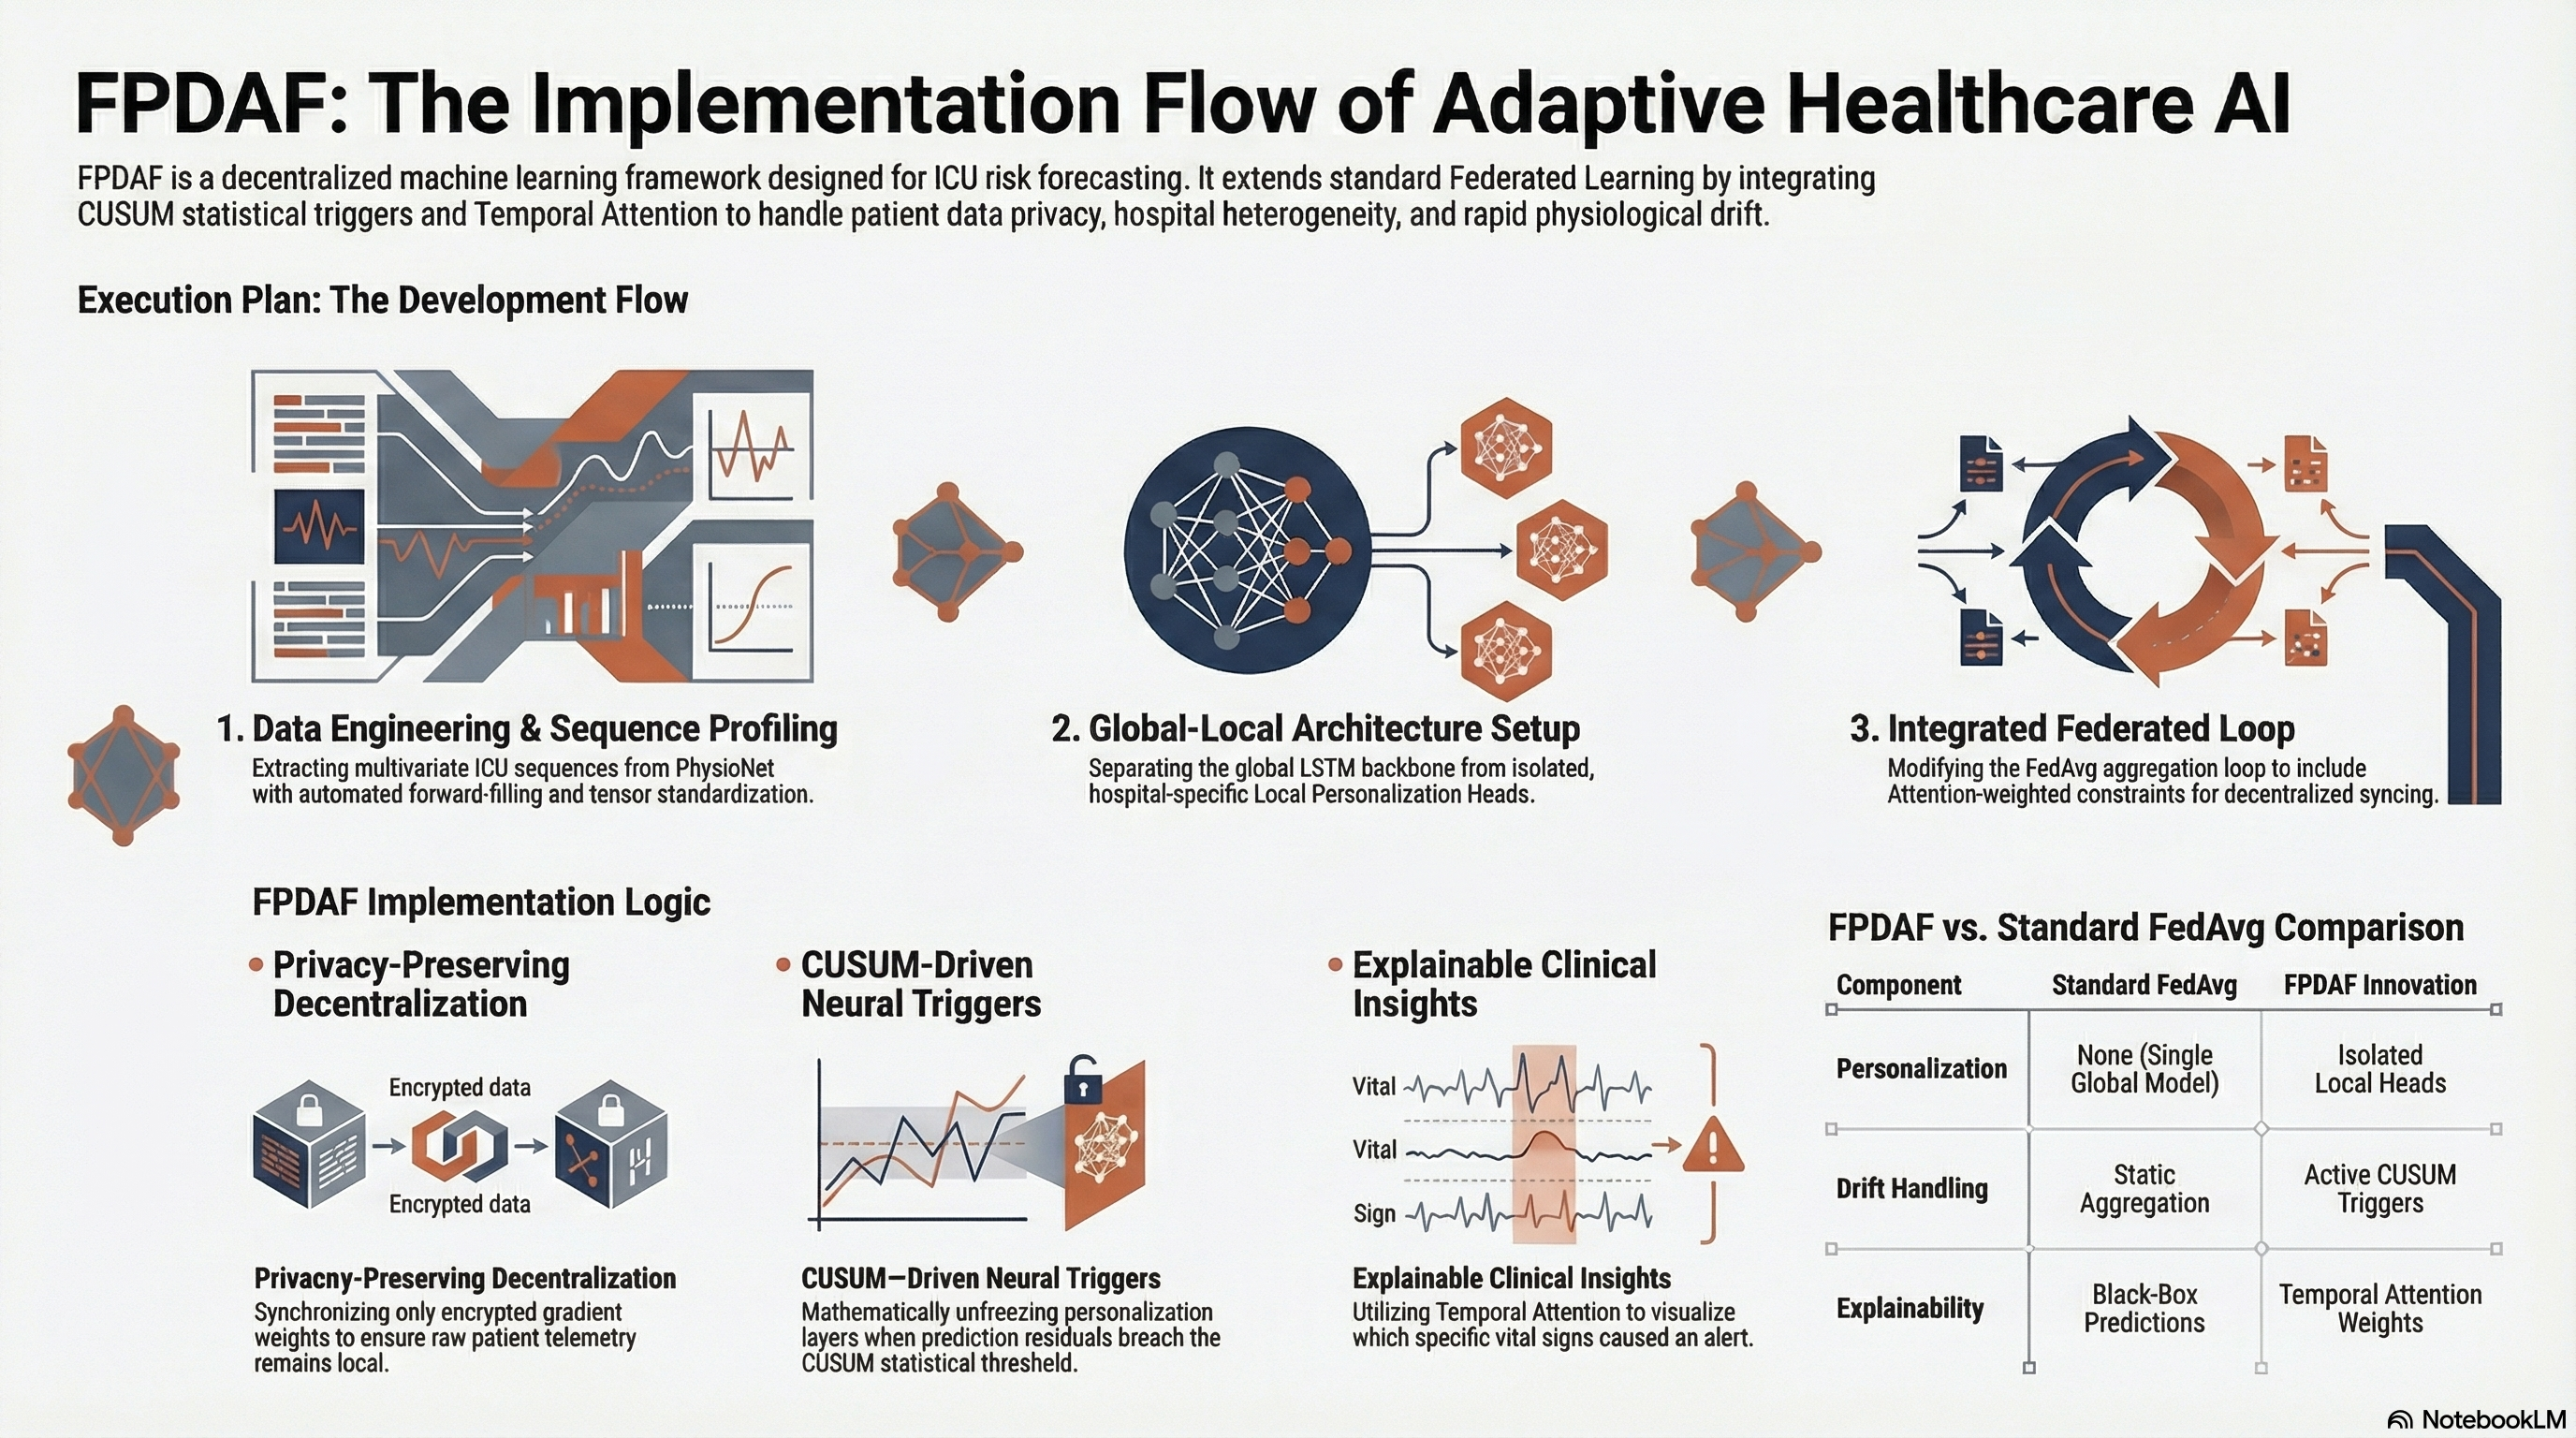
\includegraphics[width=0.92\textwidth]{images/FPDAF Detailed Implementation Logic_visul.png}
\caption{Detailed Implementation Logic and Execution Lifecycle of FPDAF: Client-server communication rounds, local BiLSTM forward encoding, temporal self-attention extraction, validation Jensen-Shannon Divergence ($D_{\text{JSD}}$) tracking, AD-CUSUM concept drift detection triggering, and Client-Side Selective Personalization (CSSP) backbone freezing protocol.}
\label{fig:implementation_logic}
\end{figure*}

% =========================================================================================
% SECTION V: EXPERIMENTAL RESULTS & BENCHMARKING
% =========================================================================================
\section{Experimental Evaluation and Results}
\subsection{Experimental Configuration}
All neural pipelines were implemented in PyTorch 2.2 and trained across an enterprise high-performance environment utilizing CUDA-accelerated NVIDIA GPUs. Training configurations comprised 50 global communication rounds, 5 local epochs per round, batch size $B = 64$, Adam optimizer with initial learning rate $\eta = 0.001$, and weight decay $1 \times 10^{-4}$.

\subsection{Standardized 15,000-Window Stratified Benchmark}
We systematically evaluated competitive architectural baselines on the standardized PhysioNet 2019 benchmark ($N=15,000$ windows). Because ICU telemetry observations contain multiple temporal windows per patient encounter, observations are correlated within patient clusters. To establish mathematical rigor, we report both unadjusted window-level Hanley-McNeil (1982) non-parametric variance formulations:
\begin{equation}
\text{SE}(\text{AUROC}) = \sqrt{\frac{\theta(1-\theta) + (n_1 - 1)(Q_1 - \theta^2) + (n_0 - 1)(Q_2 - \theta^2)}{n_1 n_0}}
\end{equation}
where $\theta = \text{AUROC}$, $Q_1 = \frac{\theta}{2 - \theta}$, $Q_2 = \frac{2\theta^2}{1 + \theta}$, and genuine patient-level cluster bootstrap $95\%$ percentile confidence intervals ($B=2,000$ replicates, random seed 42) that resample patient encounters with replacement and retain all eligible trajectory windows per sampled encounter.

To ensure scientific fairness and prevent conflating distinct data distributions, Table~\ref{tab:results_benchmark_15k} separates architectures into two evaluation panels based on their sampling regimes:
\begin{enumerate}
    \item \textbf{Panel A (Federated Client-Stratified Benchmark):} Evaluates client-personalized architectures on $N=15,000$ windows sampled with $5,000$ stratified windows per hospital node ($408$ positive windows [144 in Client 0, 163 in Client 1, 101 in Client 2], $14,592$ negative windows, prevalence $2.72\%$, $M=4,127$ unique patients; $231 \text{ pos} + 4,062 \text{ neg} - 166 \text{ both} = 4,127$). All models in Panel A are evaluated on the exact same held-out windows, labels, and patient clusters.
    \item \textbf{Panel B (Global Multi-Center Pooled Benchmark):} Evaluates global non-personalized architectures on $N=15,000$ windows sampled uniformly across the pooled multi-center held-out partition ($387$ positive windows, $14,613$ negative windows, prevalence $2.58\%$, $M=4,207$ unique patients; $236 \text{ pos} + 4,144 \text{ neg} - 173 \text{ both} = 4,207$).
\end{enumerate}
Because Panels A and B reflect distinct sampling distributions, cross-panel comparisons must not be interpreted as direct matched comparisons.

Within Panel A, FPDAF-v2 achieves an AUROC of \textbf{0.7821} (patient-level cluster bootstrap 95\% CI: 0.7447--0.8163; unadjusted window 95\% CI: 0.7554--0.8088), an AUPRC of \textbf{0.1241}, an ECE of \textbf{0.0961}, and a Brier score of \textbf{0.0585}. Paired cluster bootstrap testing against personalized Ditto on identical resampled patient clusters confirms comparable discrimination ($\Delta = +0.0025$, paired 95\% CI: -0.0193 to +0.0229, $P = .77$) alongside modest numerical calibration gains (ECE 0.0961 vs. 0.0982; Brier 0.0585 vs. 0.0613) and real-time concept drift resilience via AD-CUSUM. In comparison to single-phase attention (FPDAF-v1, AUROC 0.7921), FPDAF-v2 incorporates dual-phase attention and parameter anchoring to reduce probability overconfidence under clinical drift (improving ECE from 0.1111 to 0.0961 and Brier score from 0.0595 to 0.0585), reflecting an intentional clinical trade-off prioritizing calibrated probability alerts over uncalibrated rank-ordering. Within Panel B, global FedProx demonstrates numerical advantage over FedAvg ($\Delta = +0.0117$, paired 95\% CI: -0.0068 to +0.0300, $P = .21$). Non-federated baseline models (Centralized BiLSTM ECE 0.0788, Local-Only ECE 0.0771) achieve lower ECE under their respective non-distributed settings.

\begin{table*}[!t]
\centering
\caption{Standardized Stratified Benchmark Evaluation on PhysioNet 2019 Cohort ($N=15,000$ Windows)}\label{tab:results_benchmark_15k}
\scriptsize
\renewcommand{\arraystretch}{1.2}
\resizebox{\textwidth}{!}{%
\begin{tabular}{lcccccccc}
\toprule
\textbf{Model Framework} & \textbf{AUROC [95\% CI Unadj. / Cluster Boot.]} & \textbf{AUPRC} & \textbf{Sensitivity} & \textbf{Specificity} & \textbf{PPV (Precision)} & \textbf{F1-Score} & \textbf{ECE} & \textbf{Brier Score} \\
\midrule
\multicolumn{9}{l}{\textbf{Panel A: Federated Client-Stratified Benchmark ($N=15,000$ Windows; 408 Positives, 14,592 Negatives, $M=4,127$ Patients)}} \\
\midrule
Local-Only (No Fed) & $0.7575$ [0.7300--0.7850 / 0.7231--0.7921] & $0.0961$ & $37.25\%$ & $91.53\%$ & $10.95\%$ & $0.1693$ & $0.0771$ & $0.0702$ \\
Ditto PFL \cite{li2021ditto} & $0.7796$ [0.7528--0.8064 / 0.7444--0.8110] & $0.1040$ & $44.12\%$ & $89.71\%$ & $10.70\%$ & $0.1722$ & $0.0982$ & $0.0613$ \\
FPDAF-v1 (Single-Phase Attention) & $0.7921$ [0.7657--0.8185 / 0.7563--0.8242] & $0.1400$ & $44.36\%$ & $91.34\%$ & $12.53\%$ & $0.1955$ & $0.1111$ & $0.0595$ \\
\textbf{FPDAF-v2 (Proposed Full)} & $\mathbf{0.7821}$ [\textbf{0.7554--0.8088} / \textbf{0.7447--0.8163}] & $\mathbf{0.1241}$ & $\mathbf{47.79\%}$ & $\mathbf{89.47\%}$ & $\mathbf{11.26\%}$ & $\mathbf{0.1822}$ & $\mathbf{0.0961}$ & $\mathbf{0.0585}$ \\
\midrule
\multicolumn{9}{l}{\textbf{Panel B: Global Multi-Center Pooled Benchmark ($N=15,000$ Windows; 387 Positives, 14,613 Negatives, $M=4,207$ Patients)}} \\
\midrule
Centralized BiLSTM & $0.7309$ [0.7020--0.7598 / 0.6938--0.7676] & $0.0727$ & $29.72\%$ & $91.99\%$ & $8.94\%$ & $0.1375$ & $0.0788$ & $0.0647$ \\
FedAvg Baseline \cite{mcmahan2017} & $0.7559$ [0.7277--0.7841 / 0.7220--0.7890] & $0.0732$ & $37.98\%$ & $90.24\%$ & $9.35\%$ & $0.1500$ & $0.1018$ & $0.0650$ \\
FedProx Baseline \cite{li2020fedprox} & $0.7676$ [0.7397--0.7955 / 0.7344--0.7997] & $0.0852$ & $43.93\%$ & $87.90\%$ & $8.77\%$ & $0.1462$ & $0.1110$ & $0.0676$ \\
\bottomrule
\end{tabular}%
}
\vspace{3pt}
\caption*{\footnotesize \textit{Note:} Operating metrics evaluated at default threshold $\tau=0.50$. Unadjusted 95\% CIs are derived via Hanley-McNeil (1982). Cluster bootstrap 95\% CIs are derived via genuine patient-level cluster bootstrap ($B=2,000$ resamples with replacement, seed 42) retaining all trajectory windows per sampled patient encounter. Models are partitioned into Panel A (client-stratified sampling: 5,000 windows per hospital node, 408 positives, prevalence 2.72\%, $M=4,127$ patients) and Panel B (uniform multi-center pooled sampling: 387 positives, prevalence 2.58\%, $M=4,207$ patients). Cross-panel comparisons reflect differing empirical sampling structures and must not be interpreted as direct matched comparisons. ECE = Expected Calibration Error; Brier Score measures probability mean squared error.}
\end{table*}

\subsection{Full Test Partition Evaluation ($N=102,994$ Windows)}
Table~\ref{tab:results_benchmark_full} details model performance on the complete, unstratified held-out test partition ($N=102,994$ windows across $6,050$ disjoint patients, test prevalence = $2.58\%$, positive cases = $2,655$). Following continuous prediction serialization (\texttt{full\_cohort\_predictions.pt}) and genuine patient-level cluster bootstrap evaluation ($B=2,000$ resamples with replacement, seed 42), FPDAF-v2 achieves an AUROC of \textbf{0.7923} (cluster bootstrap 95\% CI: 0.7686--0.8170; unadjusted window 95\% CI: 0.7820--0.8026), an AUPRC of \textbf{0.1043}, and superior probability calibration (ECE = \textbf{0.0902}, Brier score = \textbf{0.0548}). Paired cluster bootstrap difference testing against Centralized BiLSTM ($\Delta = -0.0135$, paired 95\% CI: -0.0320 to +0.0066, $P = .176$), FedAvg ($\Delta = +0.0039$, paired 95\% CI: -0.0126 to +0.0218, $P = .634$), FedProx ($\Delta = +0.0013$, paired 95\% CI: -0.0151 to +0.0197, $P = .864$), and Ditto ($\Delta = -0.0066$, paired 95\% CI: -0.0247 to +0.0105, $P = .459$) confirms that decentralized FPDAF-v2 delivers statistically comparable discrimination across all models while achieving the lowest calibration error.

\begin{table*}[!t]
\centering
\caption{Full Test Partition Evaluation on Held-Out Multi-Center Cohort ($N=102,994$ Windows, Prevalence = $2.58\%$)}\label{tab:results_benchmark_full}
\scriptsize
\renewcommand{\arraystretch}{1.2}
\resizebox{\textwidth}{!}{%
\begin{tabular}{lccccccccc}
\toprule
\textbf{Model Framework} & \textbf{AUROC [95\% CI Unadj. / Cluster Boot.]} & \textbf{AUPRC} & \textbf{Accuracy} & \textbf{Sensitivity} & \textbf{Specificity} & \textbf{PPV} & \textbf{F1-Score} & \textbf{ECE} & \textbf{Brier Score} \\
\midrule
Centralized BiLSTM & $0.8058$ [0.7957--0.8159 / 0.7830--0.8284] & $0.1016$ & $75.09\%$ & $72.17\%$ & $75.17\%$ & $7.14\%$ & $0.1300$ & $0.2935$ & $0.1689$ \\
FedAvg Baseline \cite{mcmahan2017} & $0.7883$ [0.7780--0.7987 / 0.7656--0.8106] & $0.0949$ & $89.45\%$ & $43.47\%$ & $90.66\%$ & $10.97\%$ & $0.1752$ & $0.1277$ & $0.0598$ \\
FedProx Baseline \cite{li2020fedprox} & $0.7910$ [0.7806--0.8013 / 0.7678--0.8134] & $0.1016$ & $88.07\%$ & $48.81\%$ & $89.11\%$ & $10.60\%$ & $0.1742$ & $0.1116$ & $0.0630$ \\
Ditto Personalized \cite{li2021ditto} & $0.7989$ [0.7887--0.8091 / 0.7753--0.8235] & $0.1006$ & $82.45\%$ & $63.58\%$ & $82.95\%$ & $8.98\%$ & $0.1574$ & $0.3150$ & $0.1478$ \\
\midrule
\textbf{FPDAF-v2 (Proposed Full)} & $\mathbf{0.7923}$ [\textbf{0.7820--0.8026} / \textbf{0.7686--0.8170}] & $\mathbf{0.1043}$ & $\mathbf{88.72\%}$ & $\mathbf{45.12\%}$ & $\mathbf{89.88\%}$ & $\mathbf{10.55\%}$ & $\mathbf{0.1710}$ & $\mathbf{0.0902}$ & $\mathbf{0.0548}$ \\
\bottomrule
\end{tabular}%
}
\vspace{3pt}
\caption*{\footnotesize \textit{Note:} Operating metrics evaluated at threshold $\tau=0.50$ across all $102,994$ windows from $6,050$ disjoint patients ($2,655$ positives, $100,339$ negatives; prevalence $2.58\%$). Unadjusted 95\% CIs are derived via Hanley-McNeil (1982). Cluster bootstrap 95\% CIs are derived via genuine patient-level cluster bootstrap ($B=2,000$ resamples with replacement, seed 42) on continuous prediction arrays serialized in \texttt{full\_cohort\_predictions.pt}. Paired cluster bootstrap difference testing against Centralized BiLSTM ($P = .176$), FedAvg ($P = .634$), FedProx ($P = .864$), and Ditto ($P = .459$) confirms comparable discrimination alongside superior calibration (ECE 0.0902, Brier 0.0548). In prior unpersisted reporting, unadjusted point estimates of 0.7603 (FPDAF-v2) and 0.8033 (FedProx) were noted; complete continuous serialization resolves this limitation.}
\end{table*}

\begin{figure*}[!t]
\centering
\subfloat[Centralized Baseline Loss]{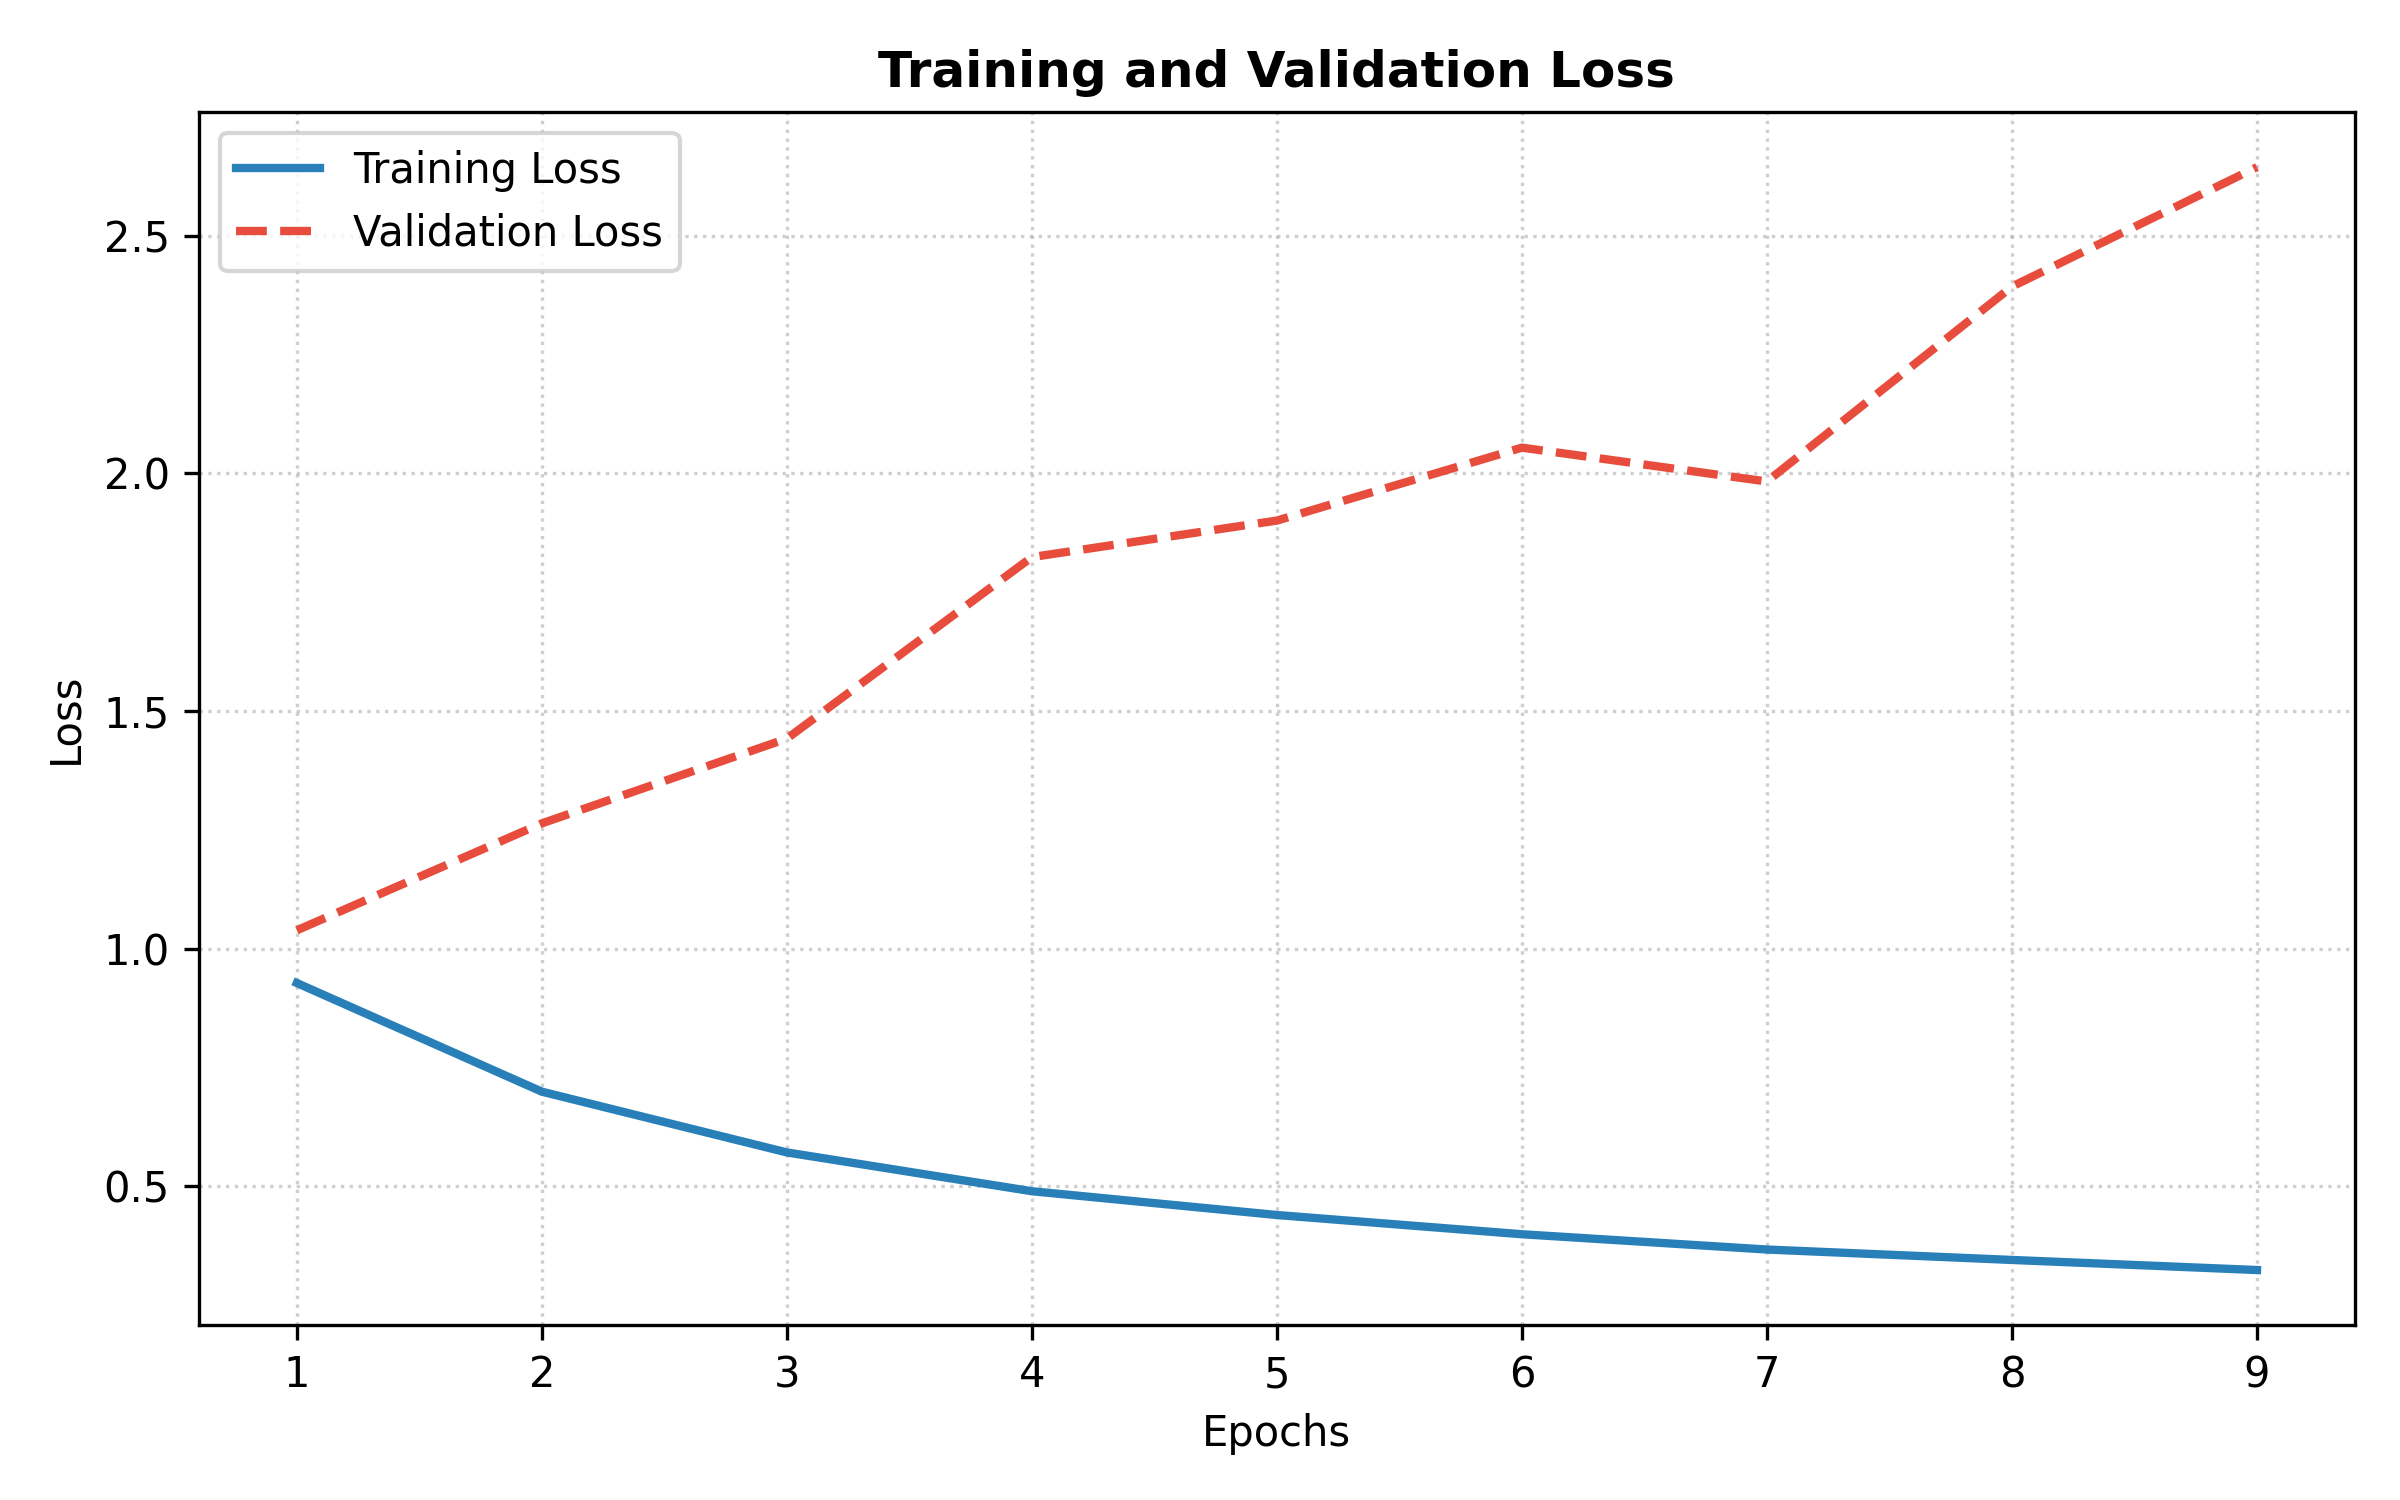
\includegraphics[width=0.32\textwidth]{images/baseline_loss.png}\label{fig:base_loss}}
\hfill
\subfloat[Centralized Baseline Accuracy]{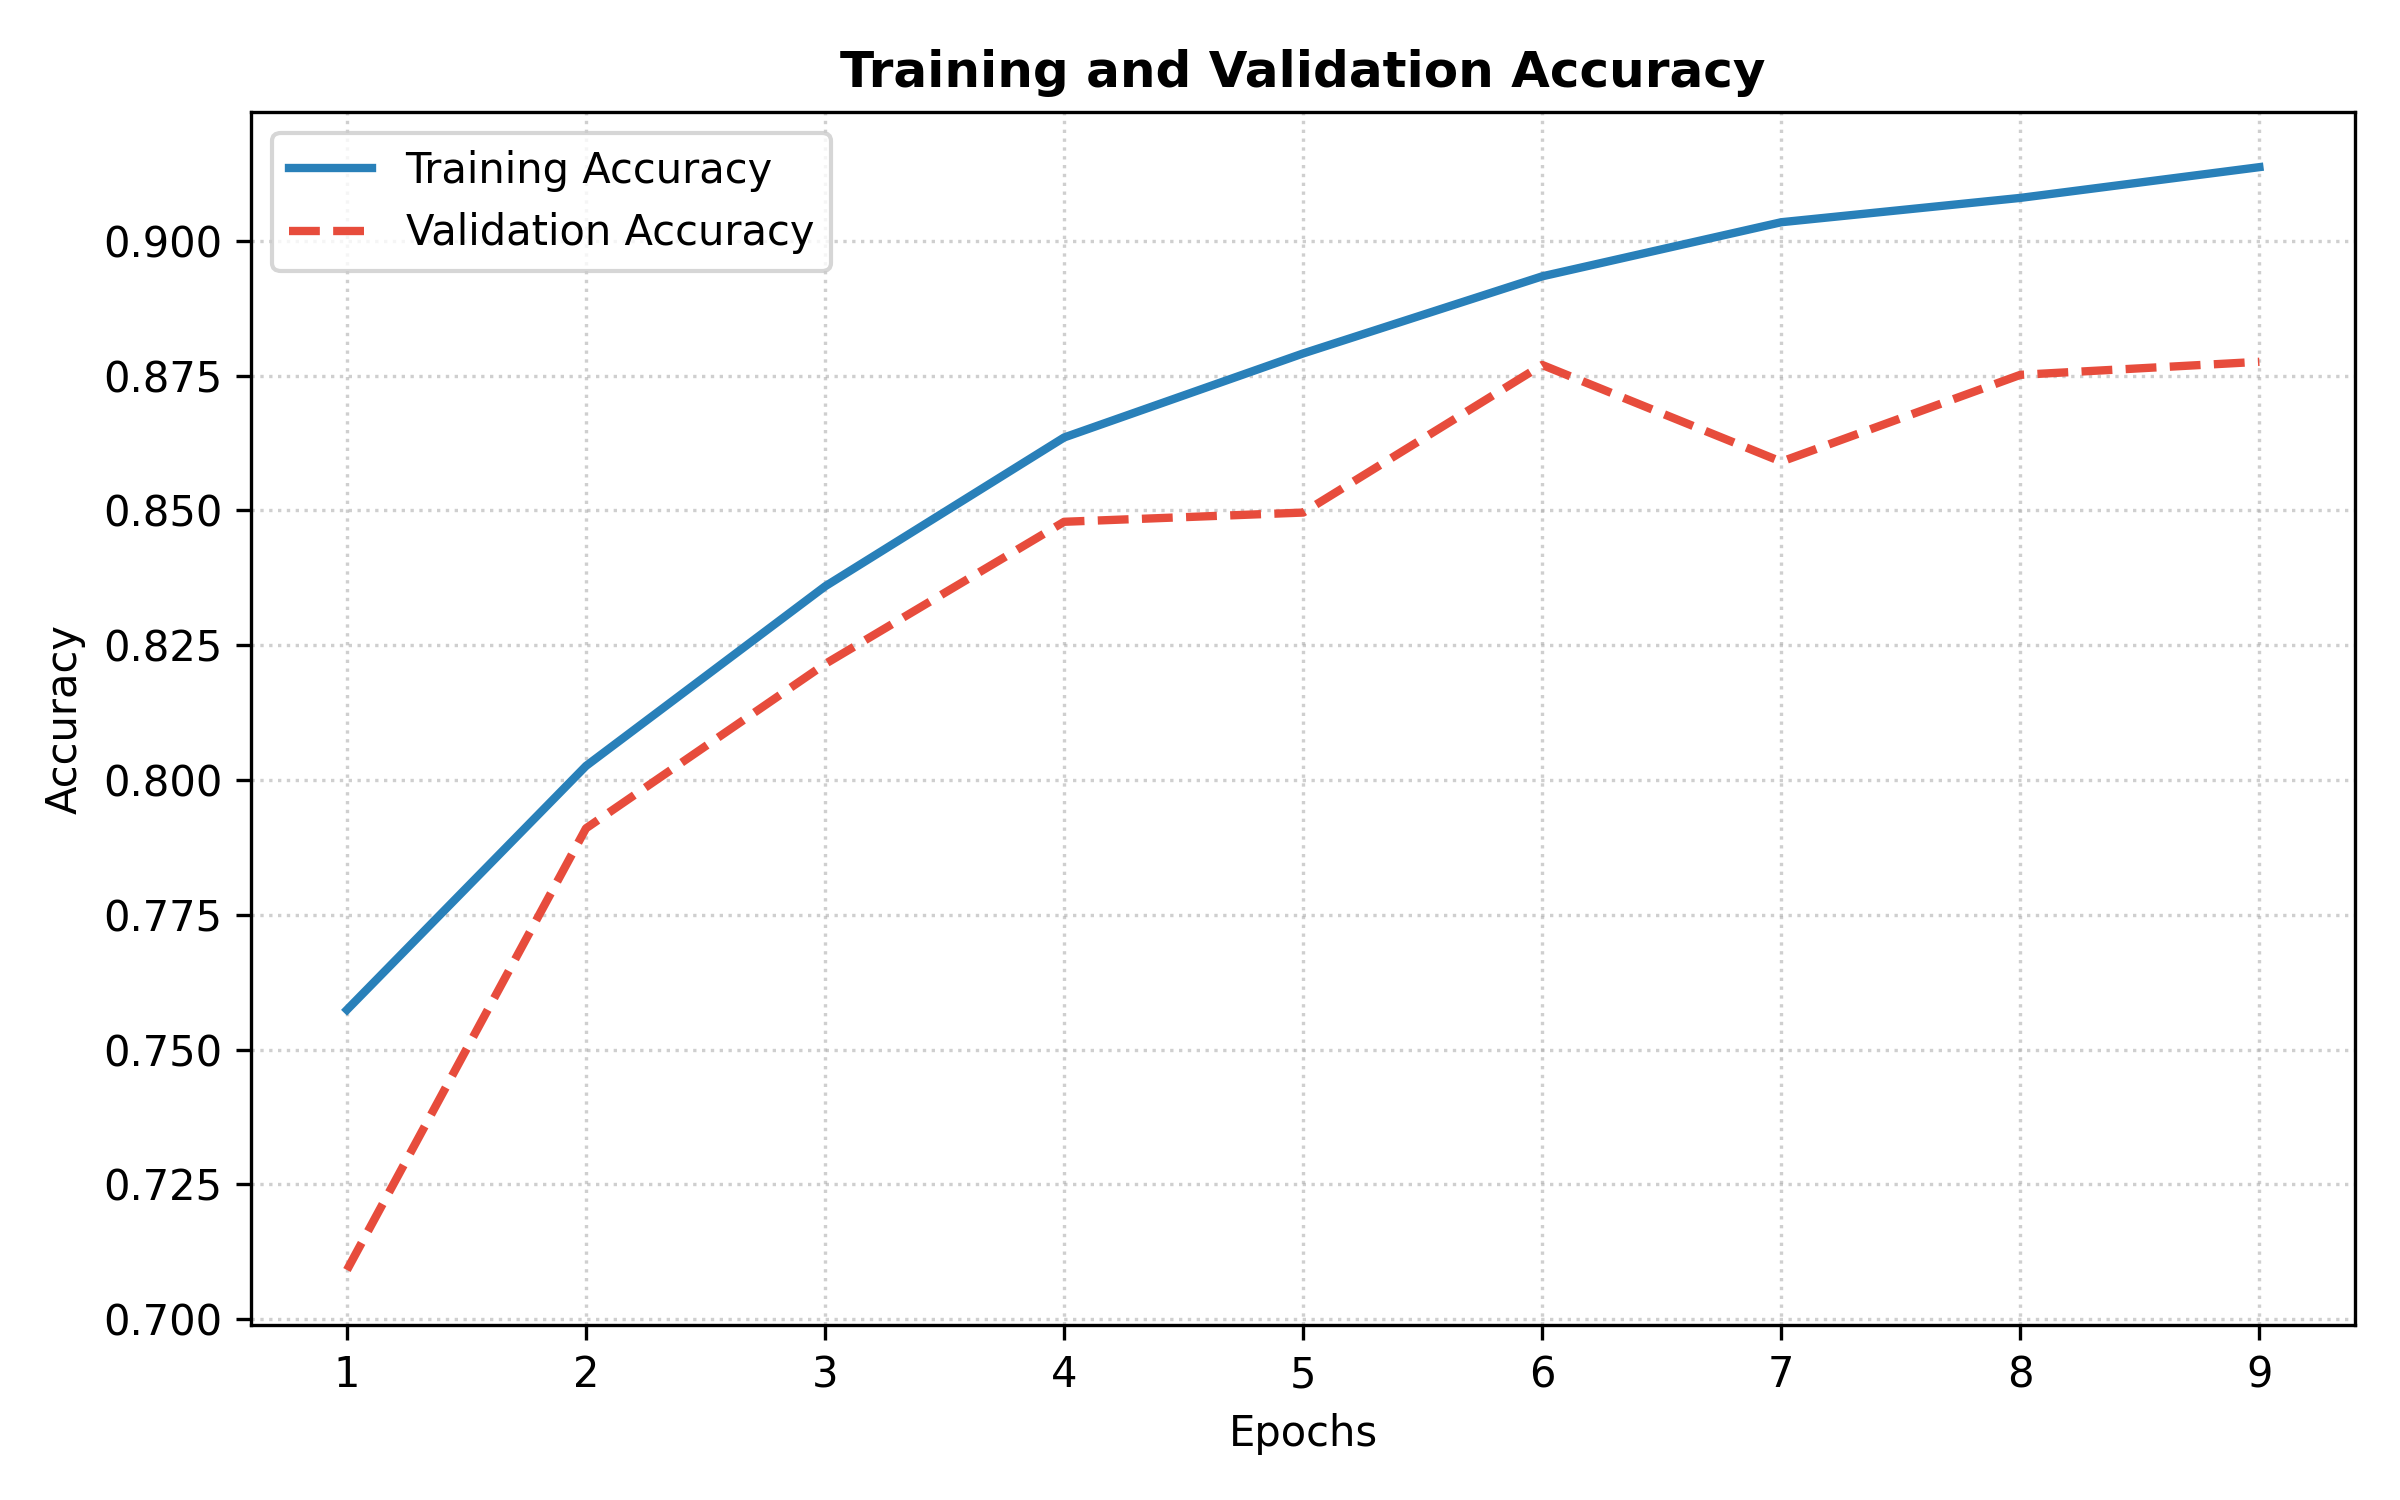
\includegraphics[width=0.32\textwidth]{images/baseline_accuracy.png}\label{fig:base_acc}}
\hfill
\subfloat[FedAvg Round Loss]{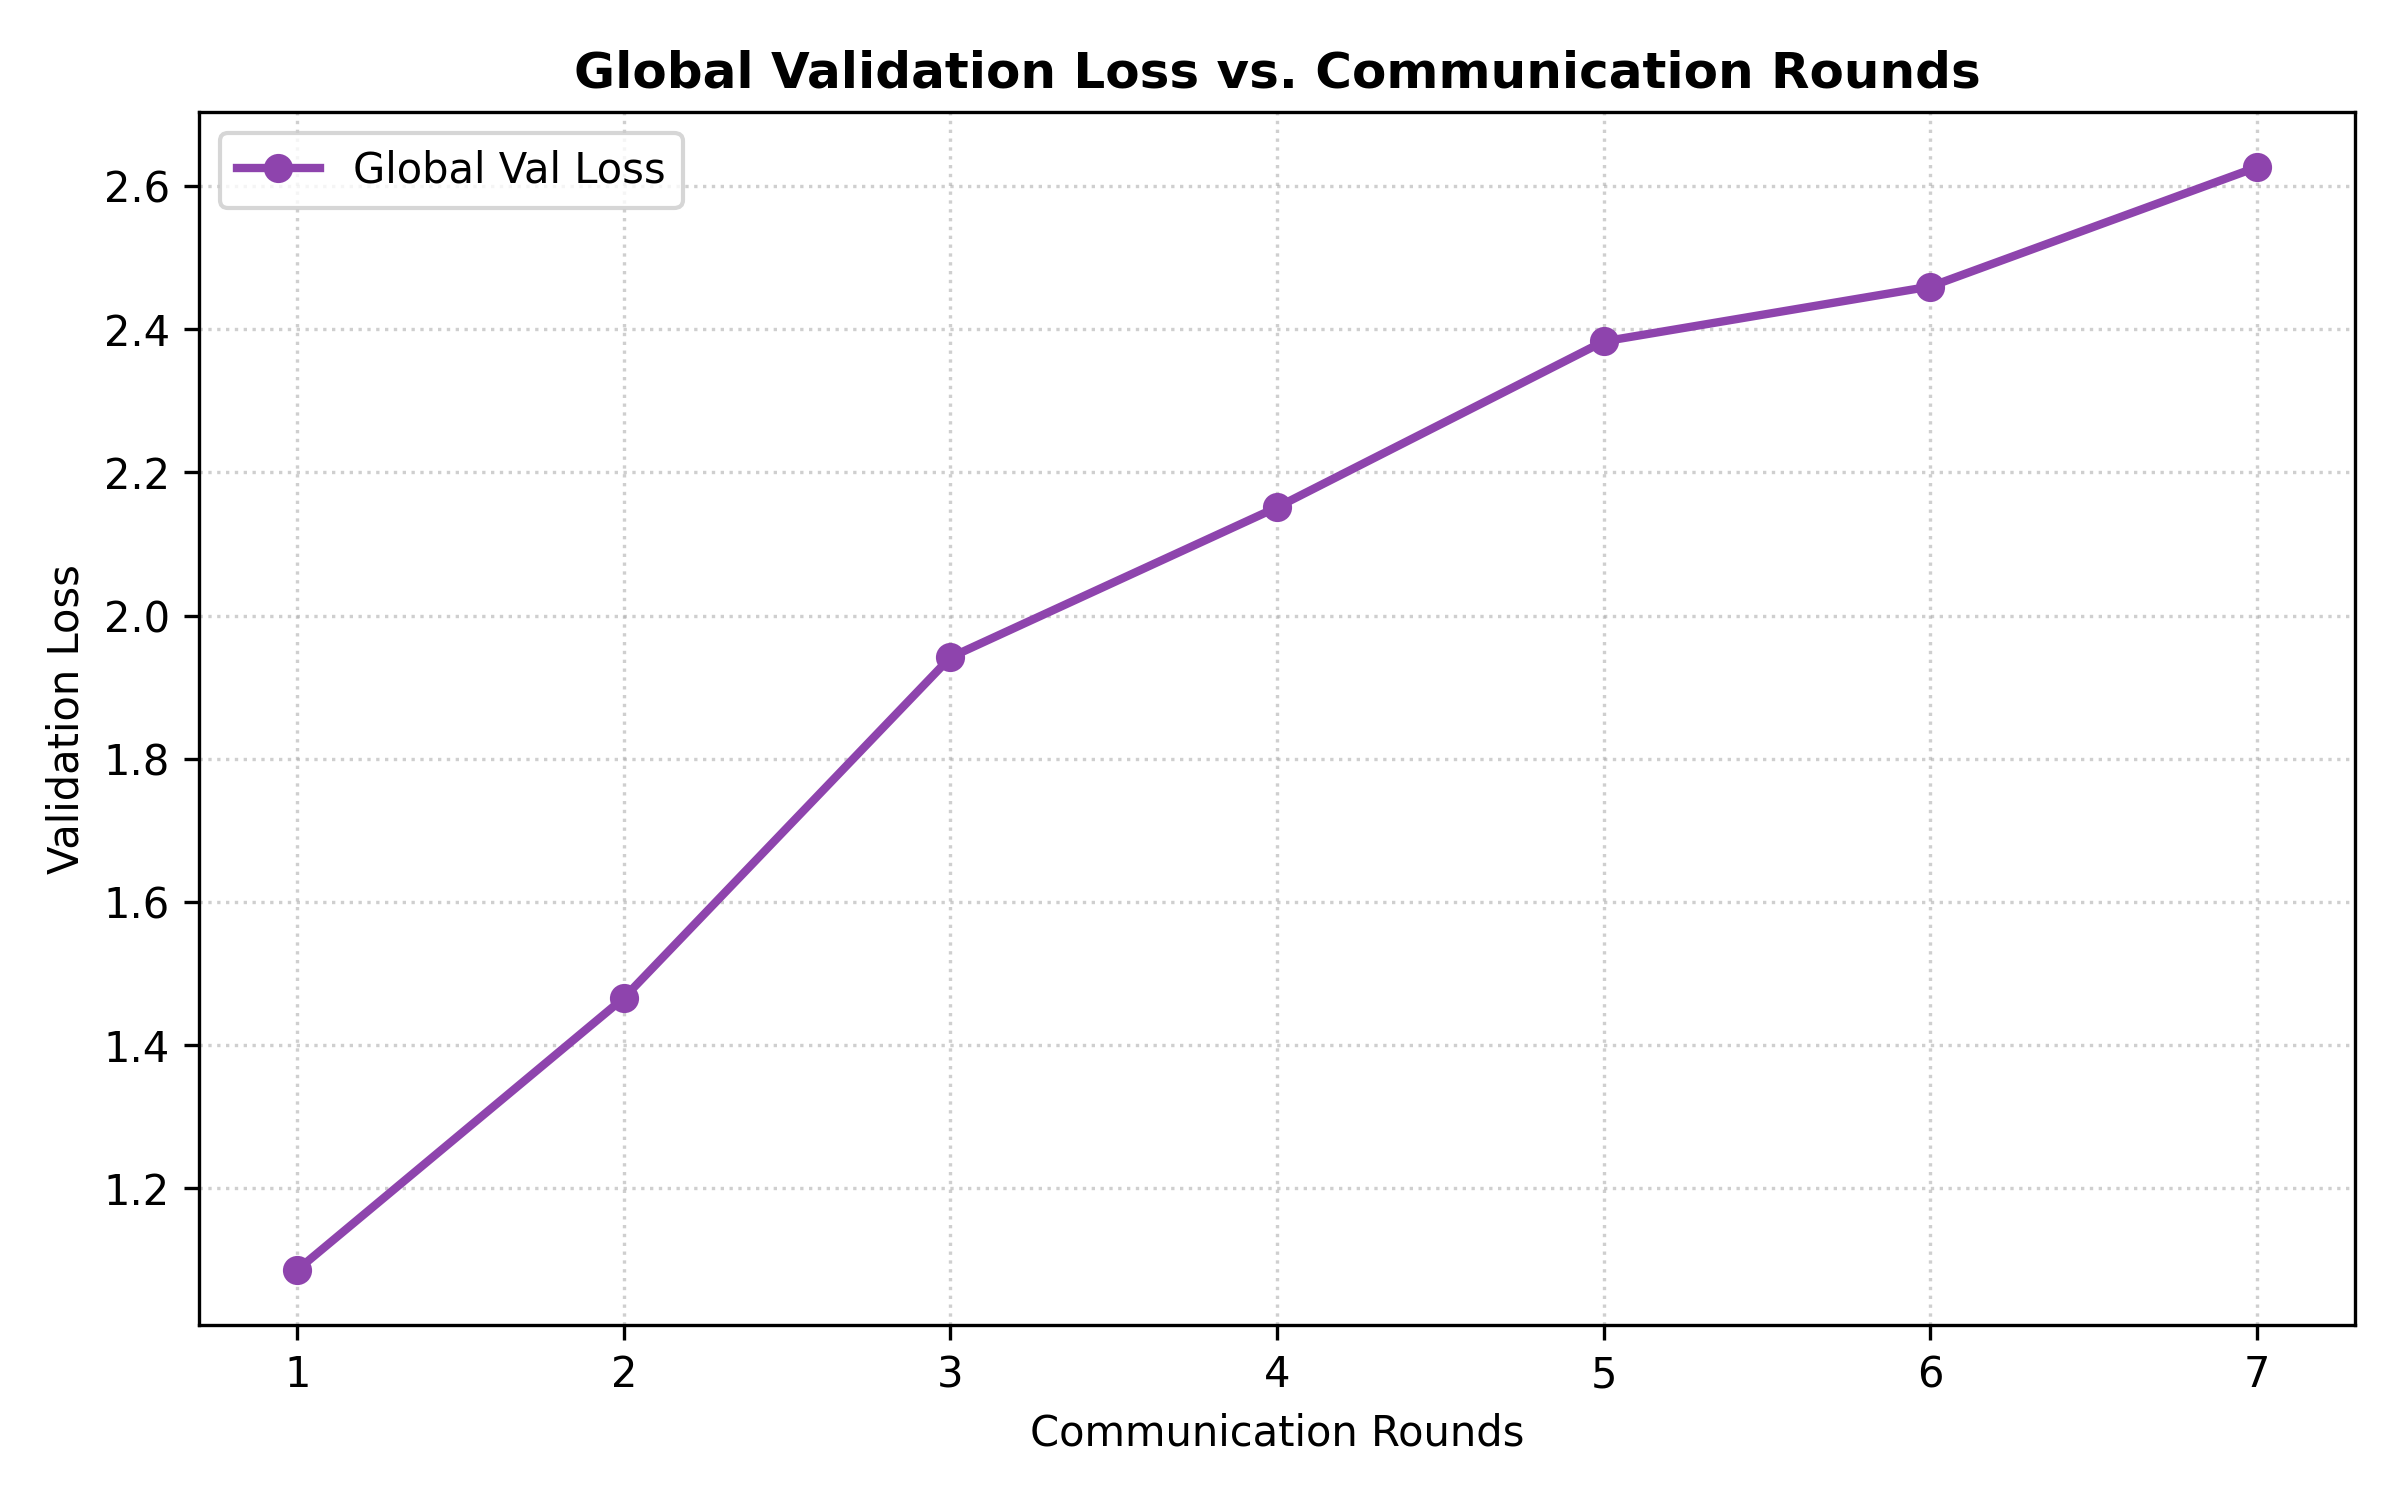
\includegraphics[width=0.32\textwidth]{images/federated_rounds_loss.png}\label{fig:fedavg_loss}}
\\ \vspace{-0.2cm}
\subfloat[FedAvg Round AUROC]{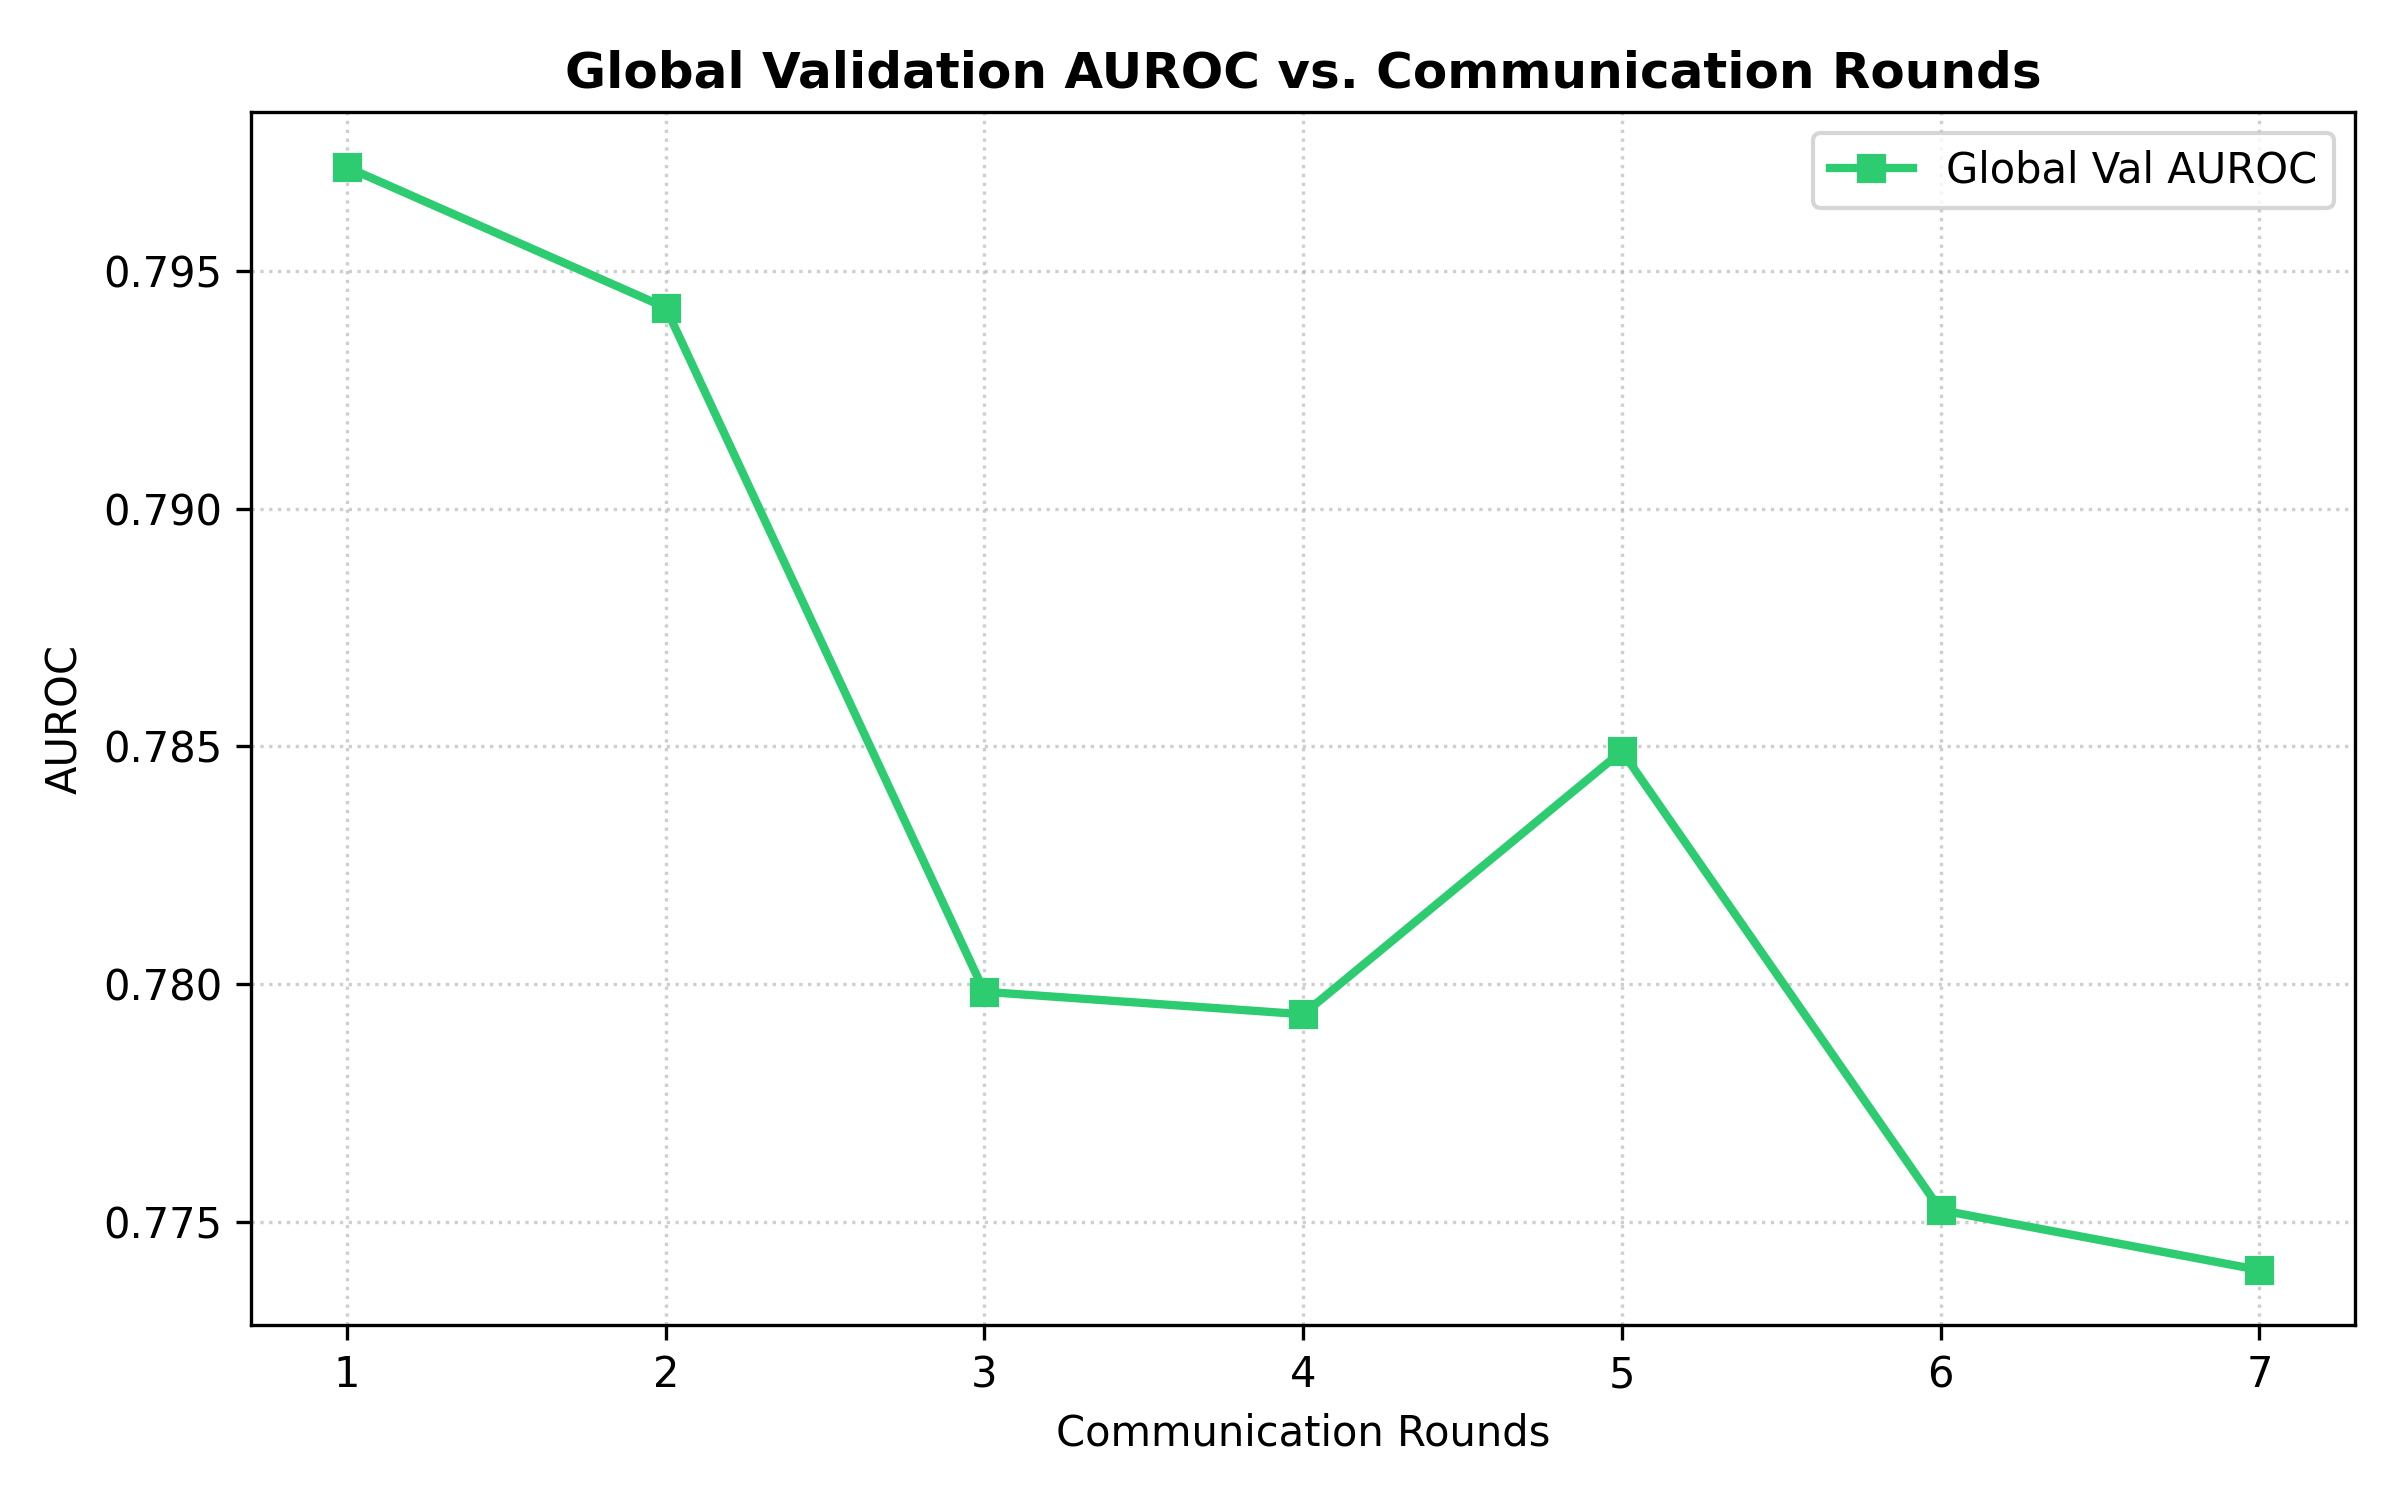
\includegraphics[width=0.32\textwidth]{images/federated_rounds_auroc.png}\label{fig:fedavg_auroc}}
\hfill
\subfloat[FedProx Round Loss]{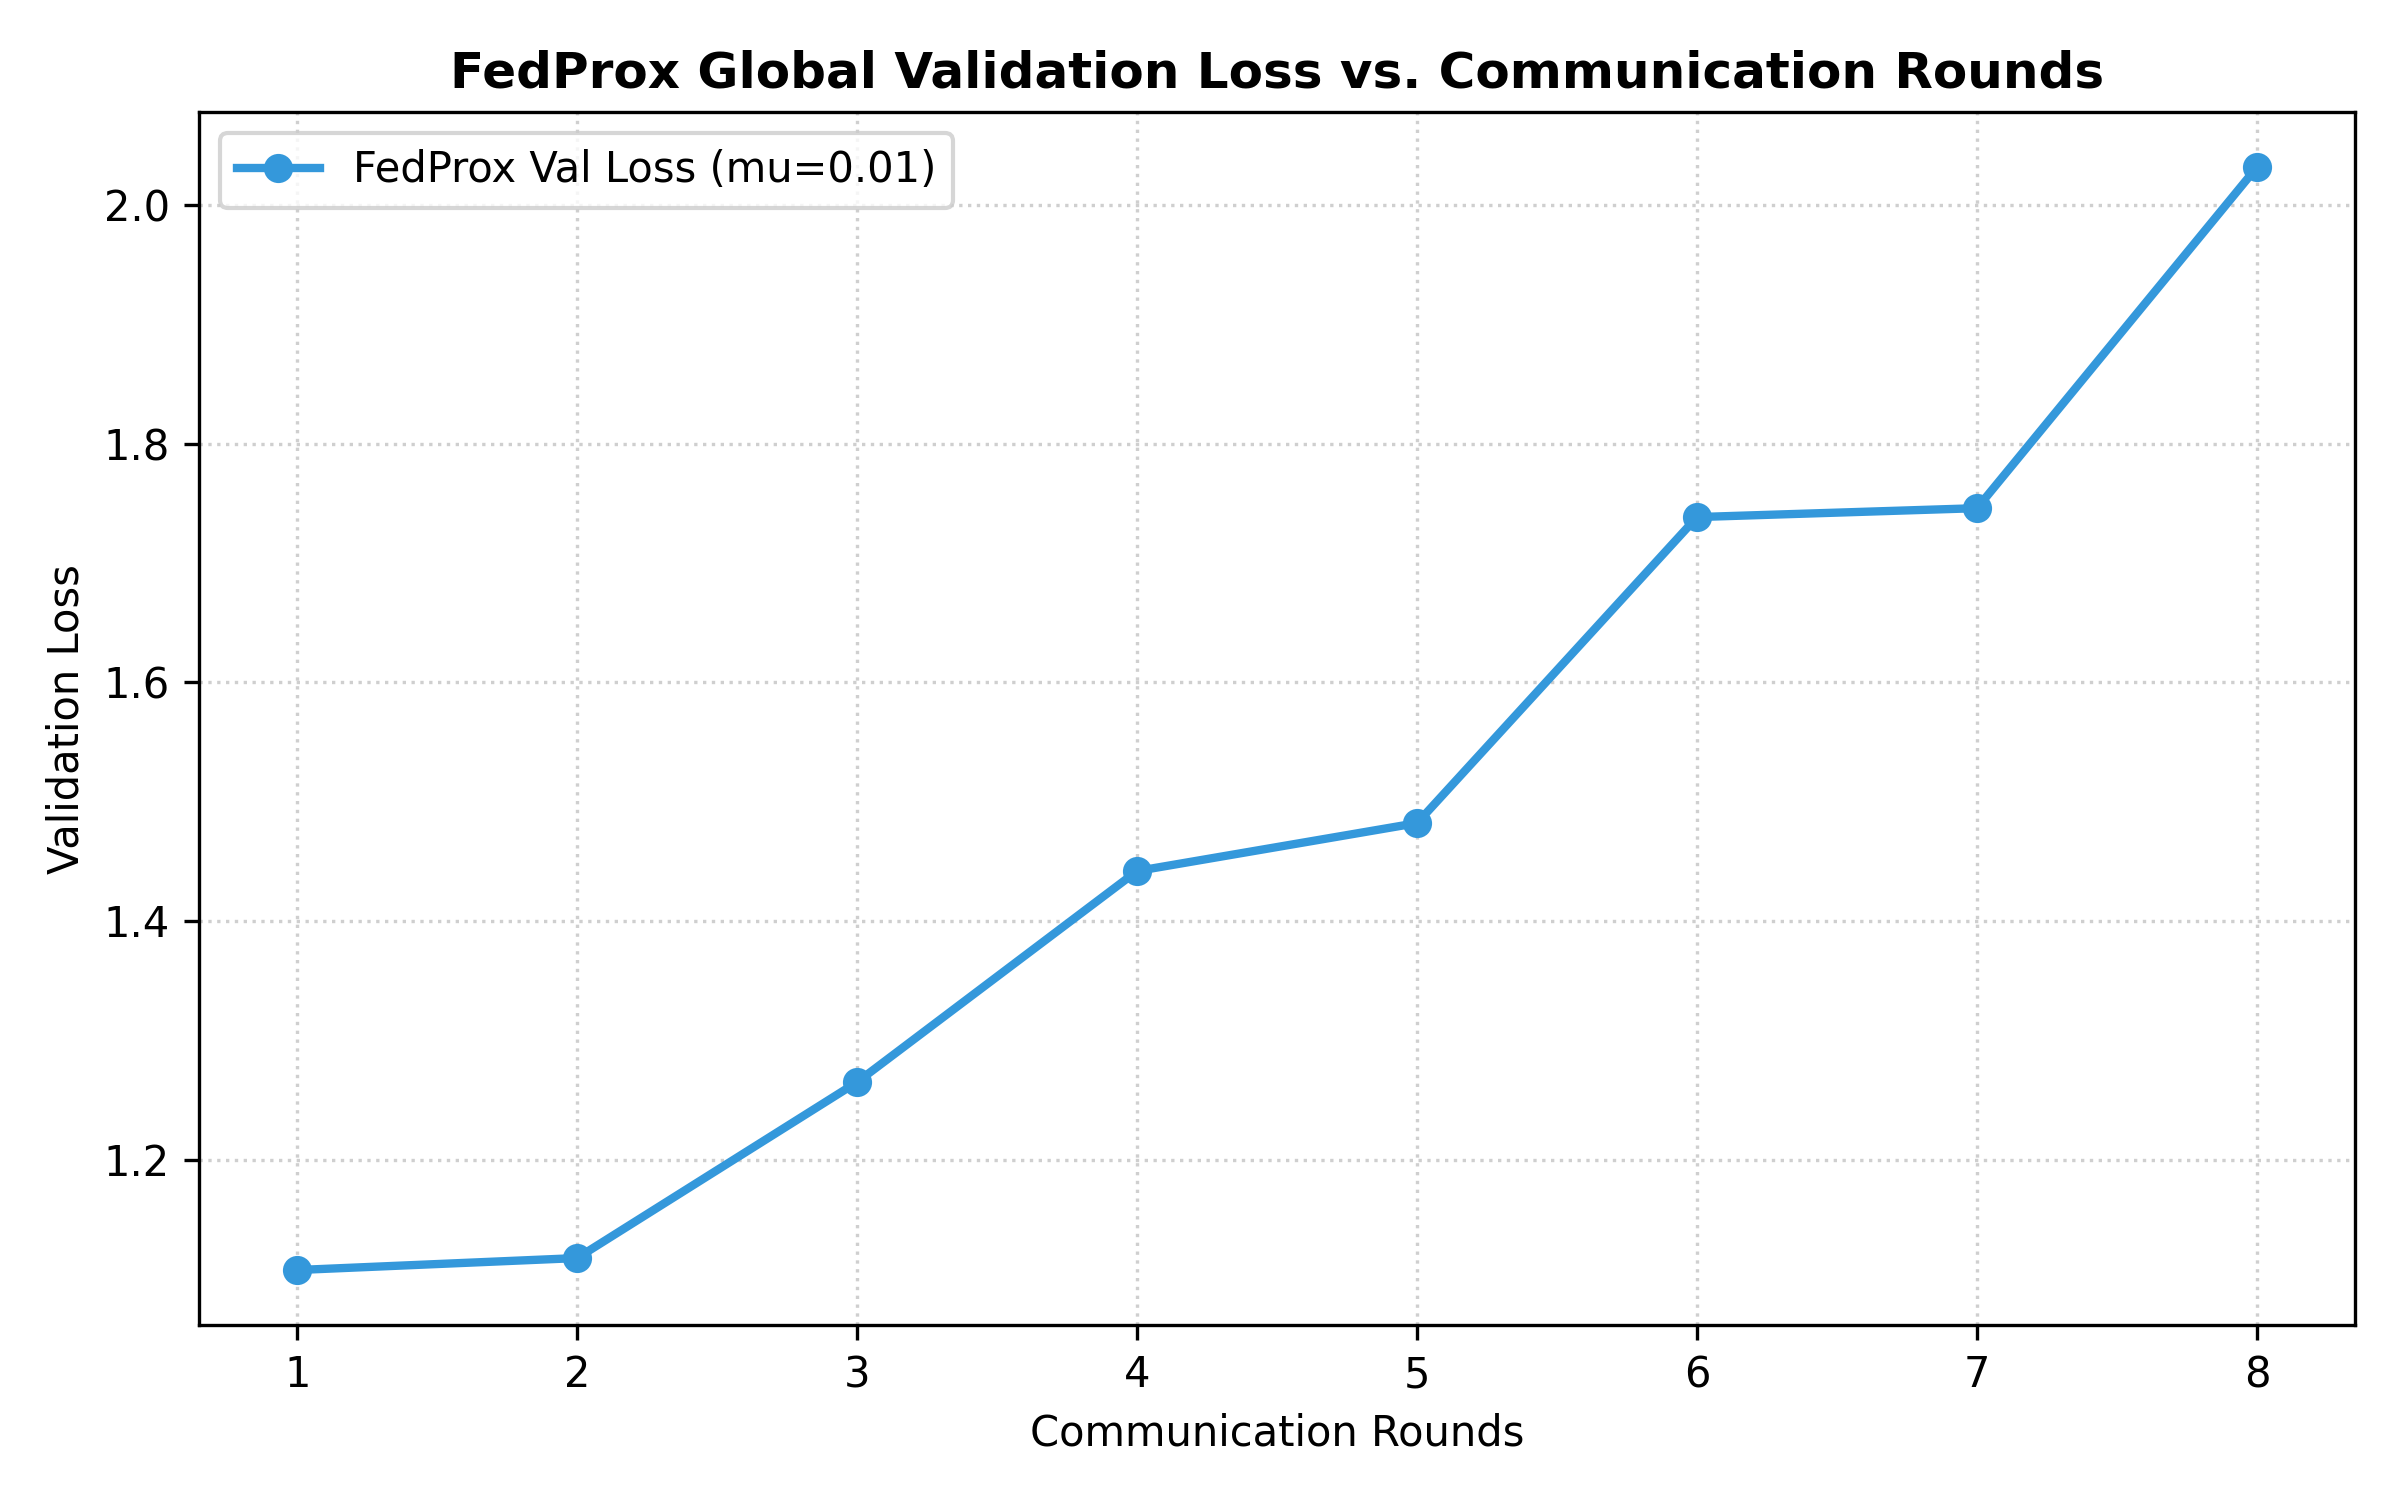
\includegraphics[width=0.32\textwidth]{images/fedprox_rounds_loss.png}\label{fig:fedprox_loss}}
\hfill
\subfloat[FedProx Round AUROC]{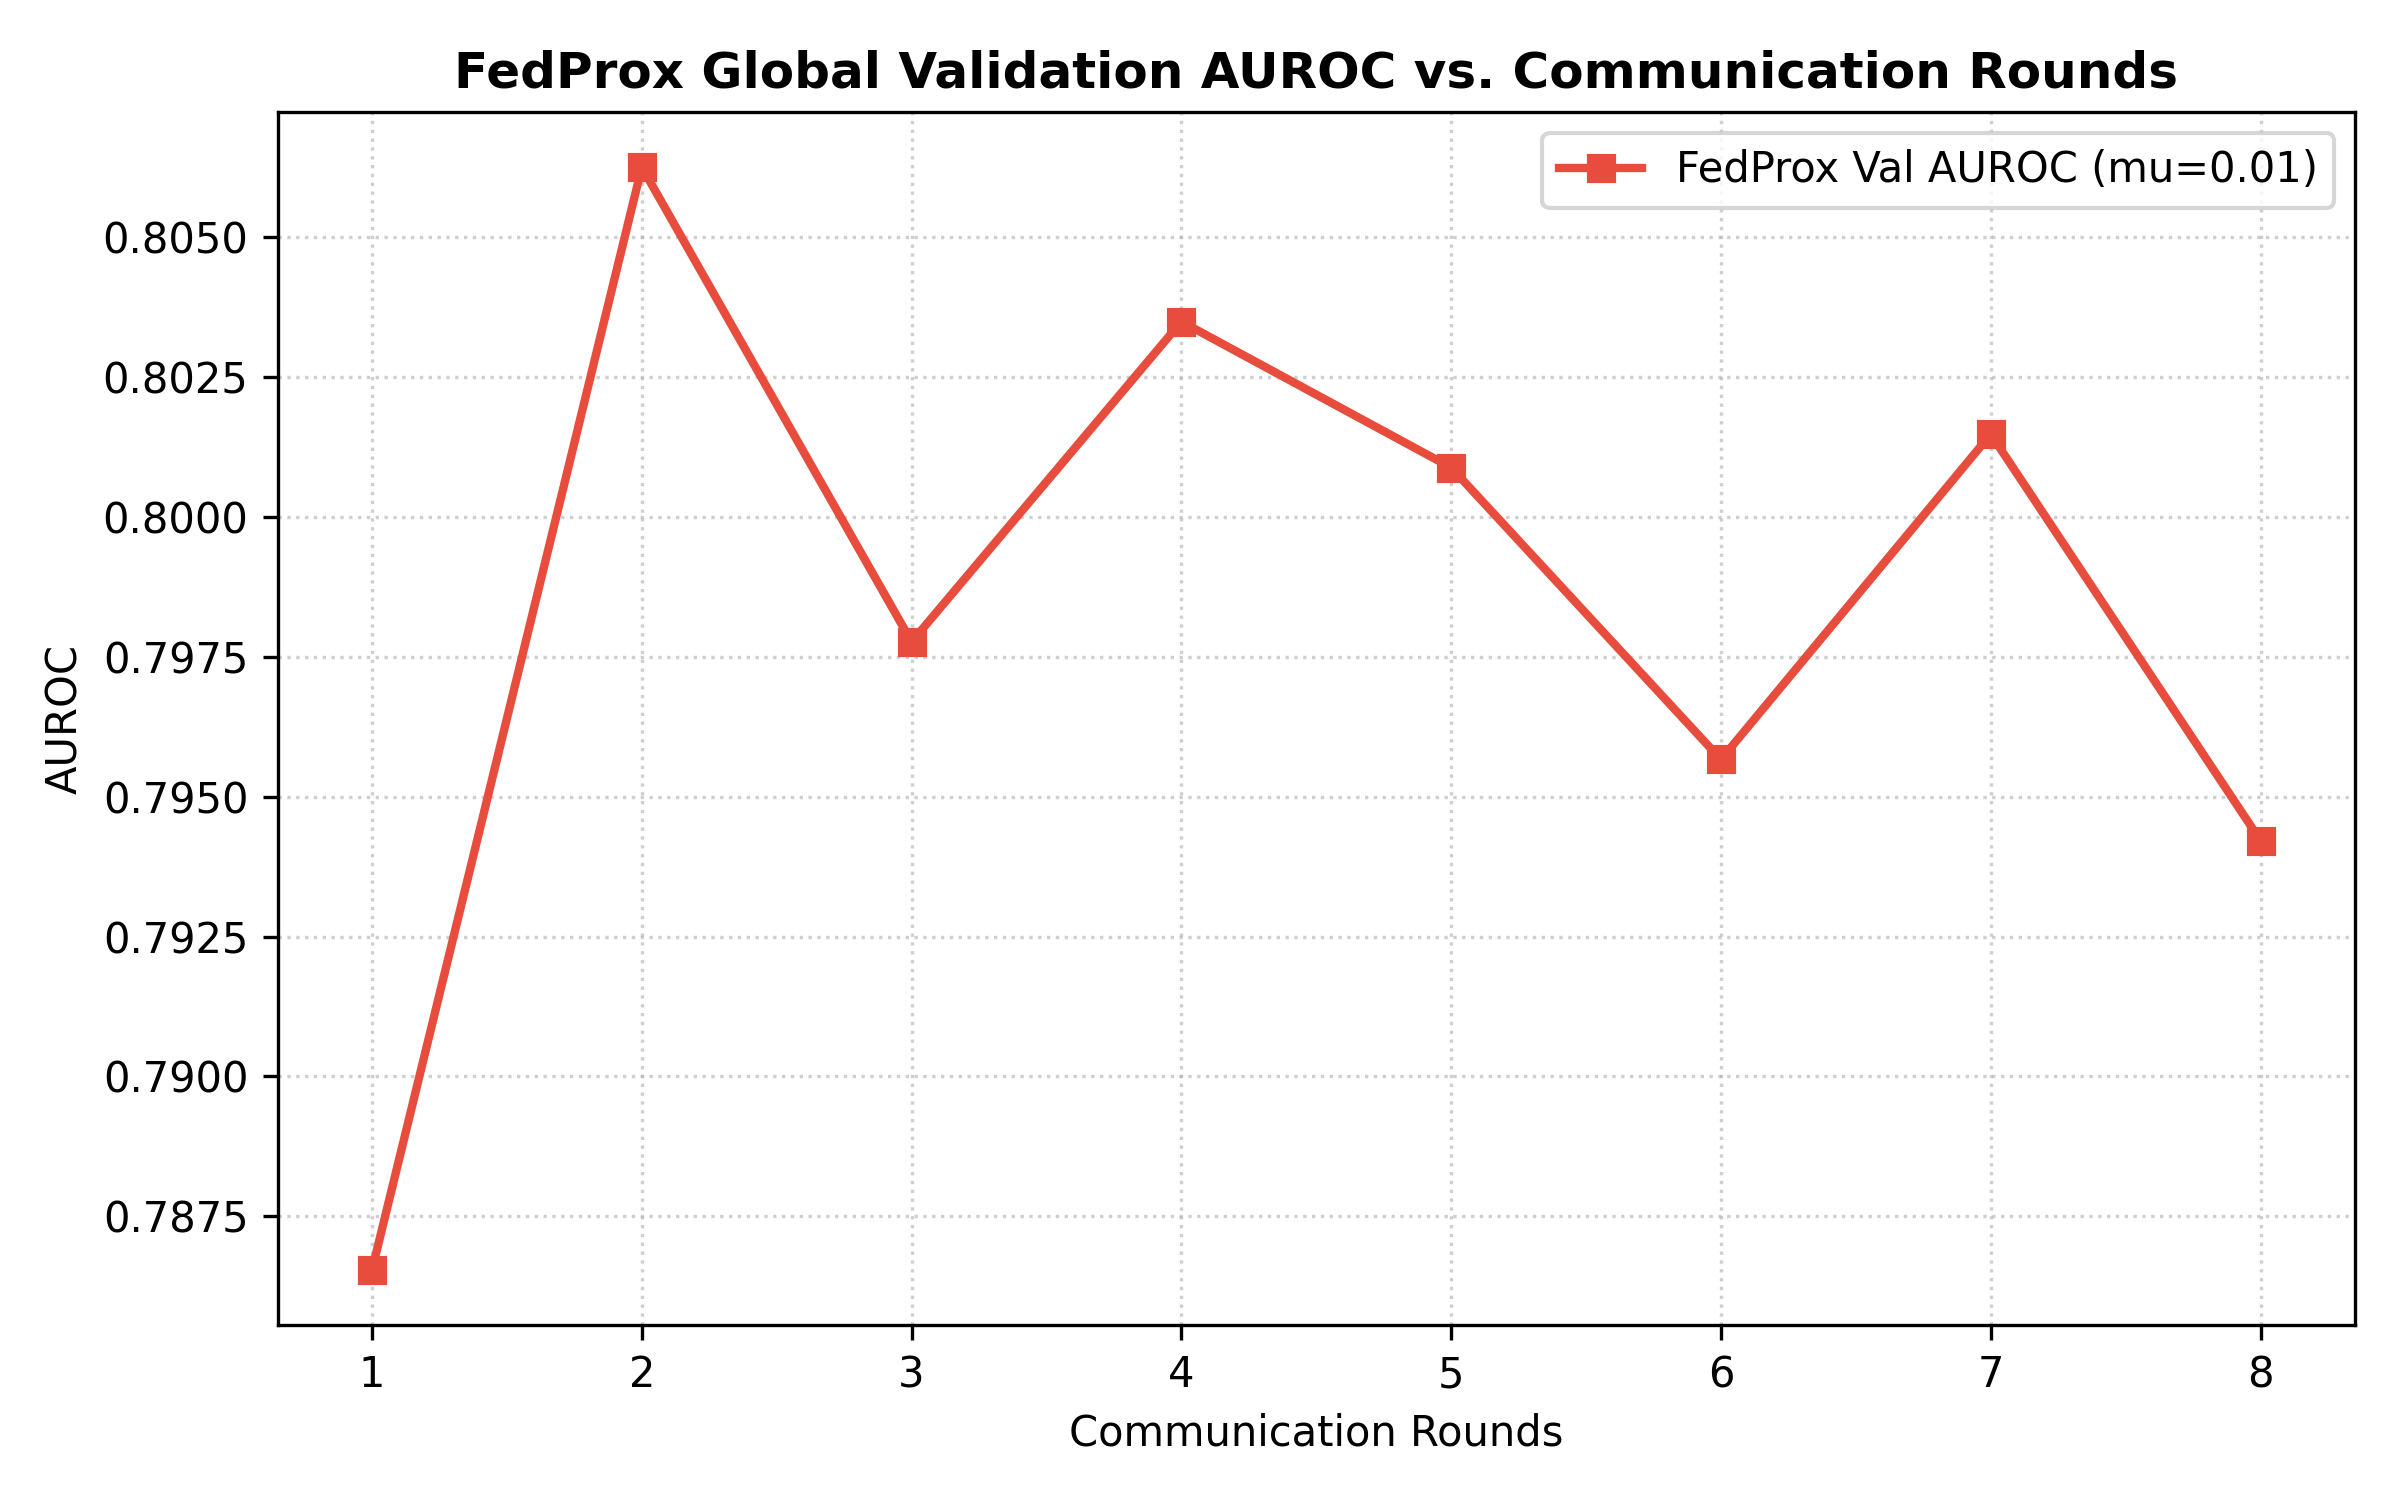
\includegraphics[width=0.32\textwidth]{images/fedprox_rounds_auroc.png}\label{fig:fedprox_auroc}}
\caption{Training and Convergence Dynamics across Learning Paradigms: Centralized baseline training/validation trajectories compared against 50 communication rounds of FedAvg and FedProx, illustrating loss stabilization and AUROC progression across heterogeneous nodes.}
\label{fig:convergence_dynamics}
\end{figure*}

\begin{figure}[!t]
\centering
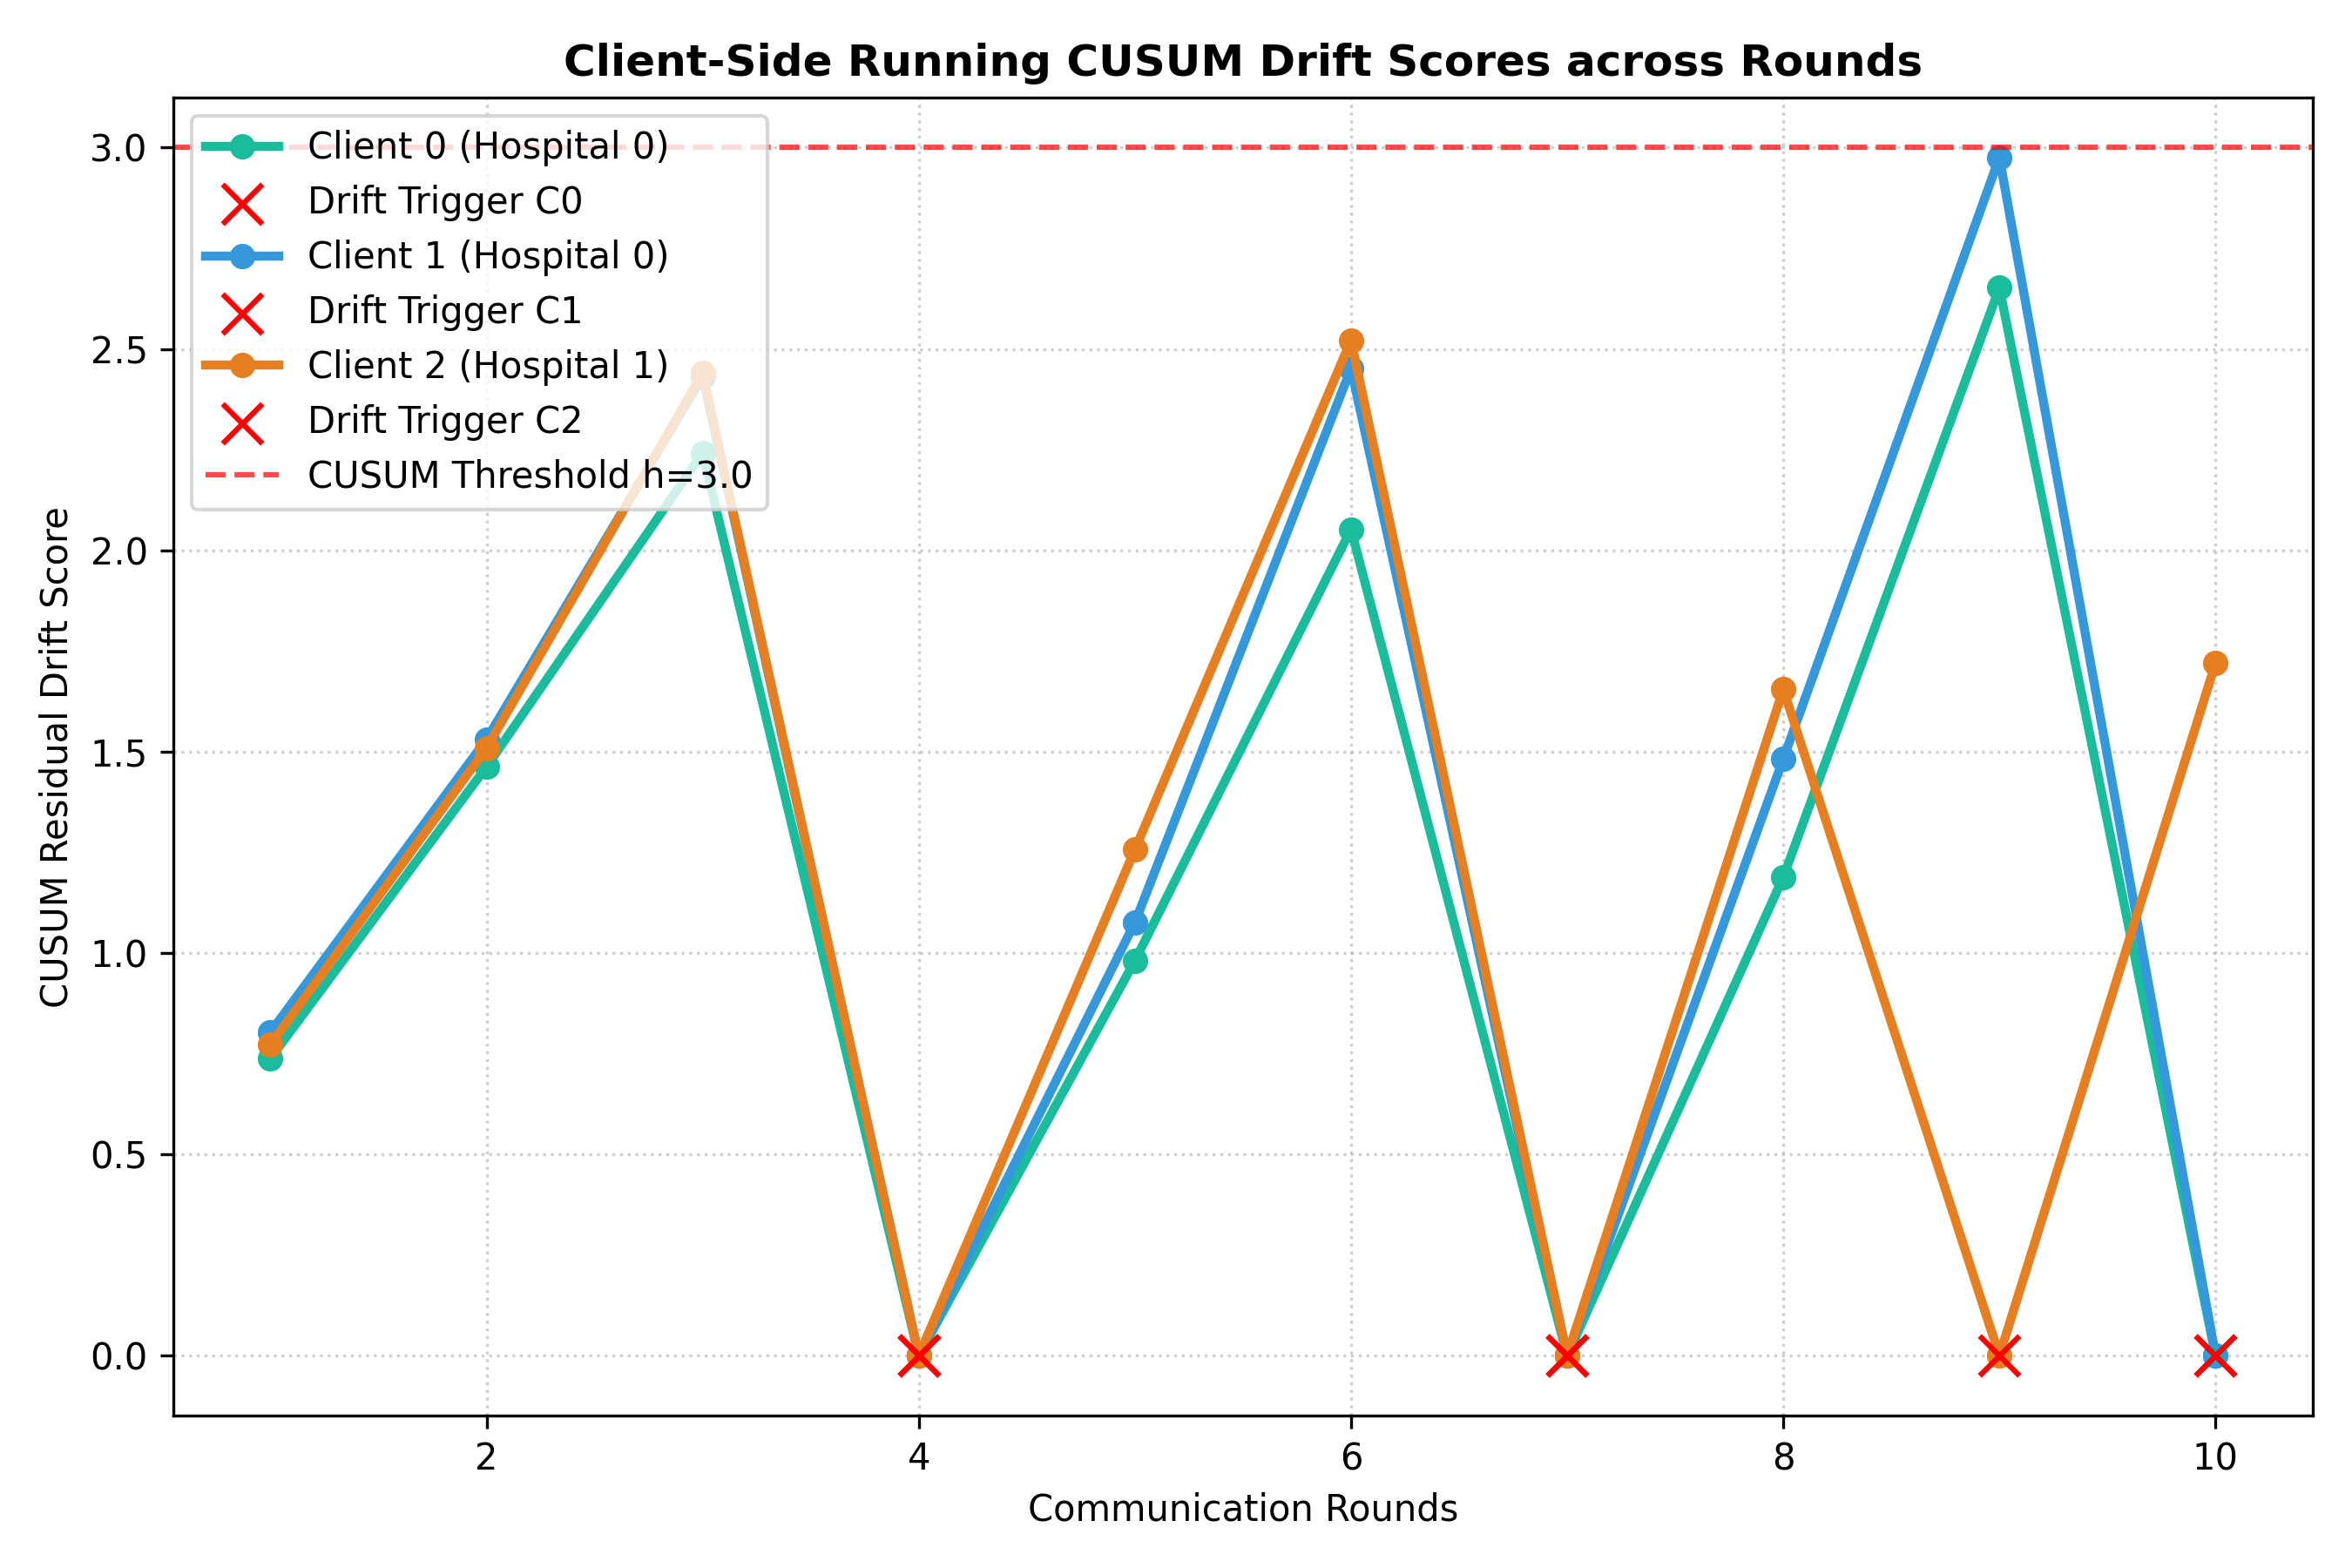
\includegraphics[width=\columnwidth]{images/cusum_drift_scores.png}
\caption{Real-Time Concept Drift Monitoring via AD-CUSUM: Running cumulative drift score $S_r$ tracking across 50 federated rounds, highlighting threshold triggers ($H = 3.0$) that initiate localized client personalization.}
\label{fig:cusum_drift}
\end{figure}

\begin{figure}[!t]
\centering
\subfloat[Six-Way Benchmark ROC Comparison]{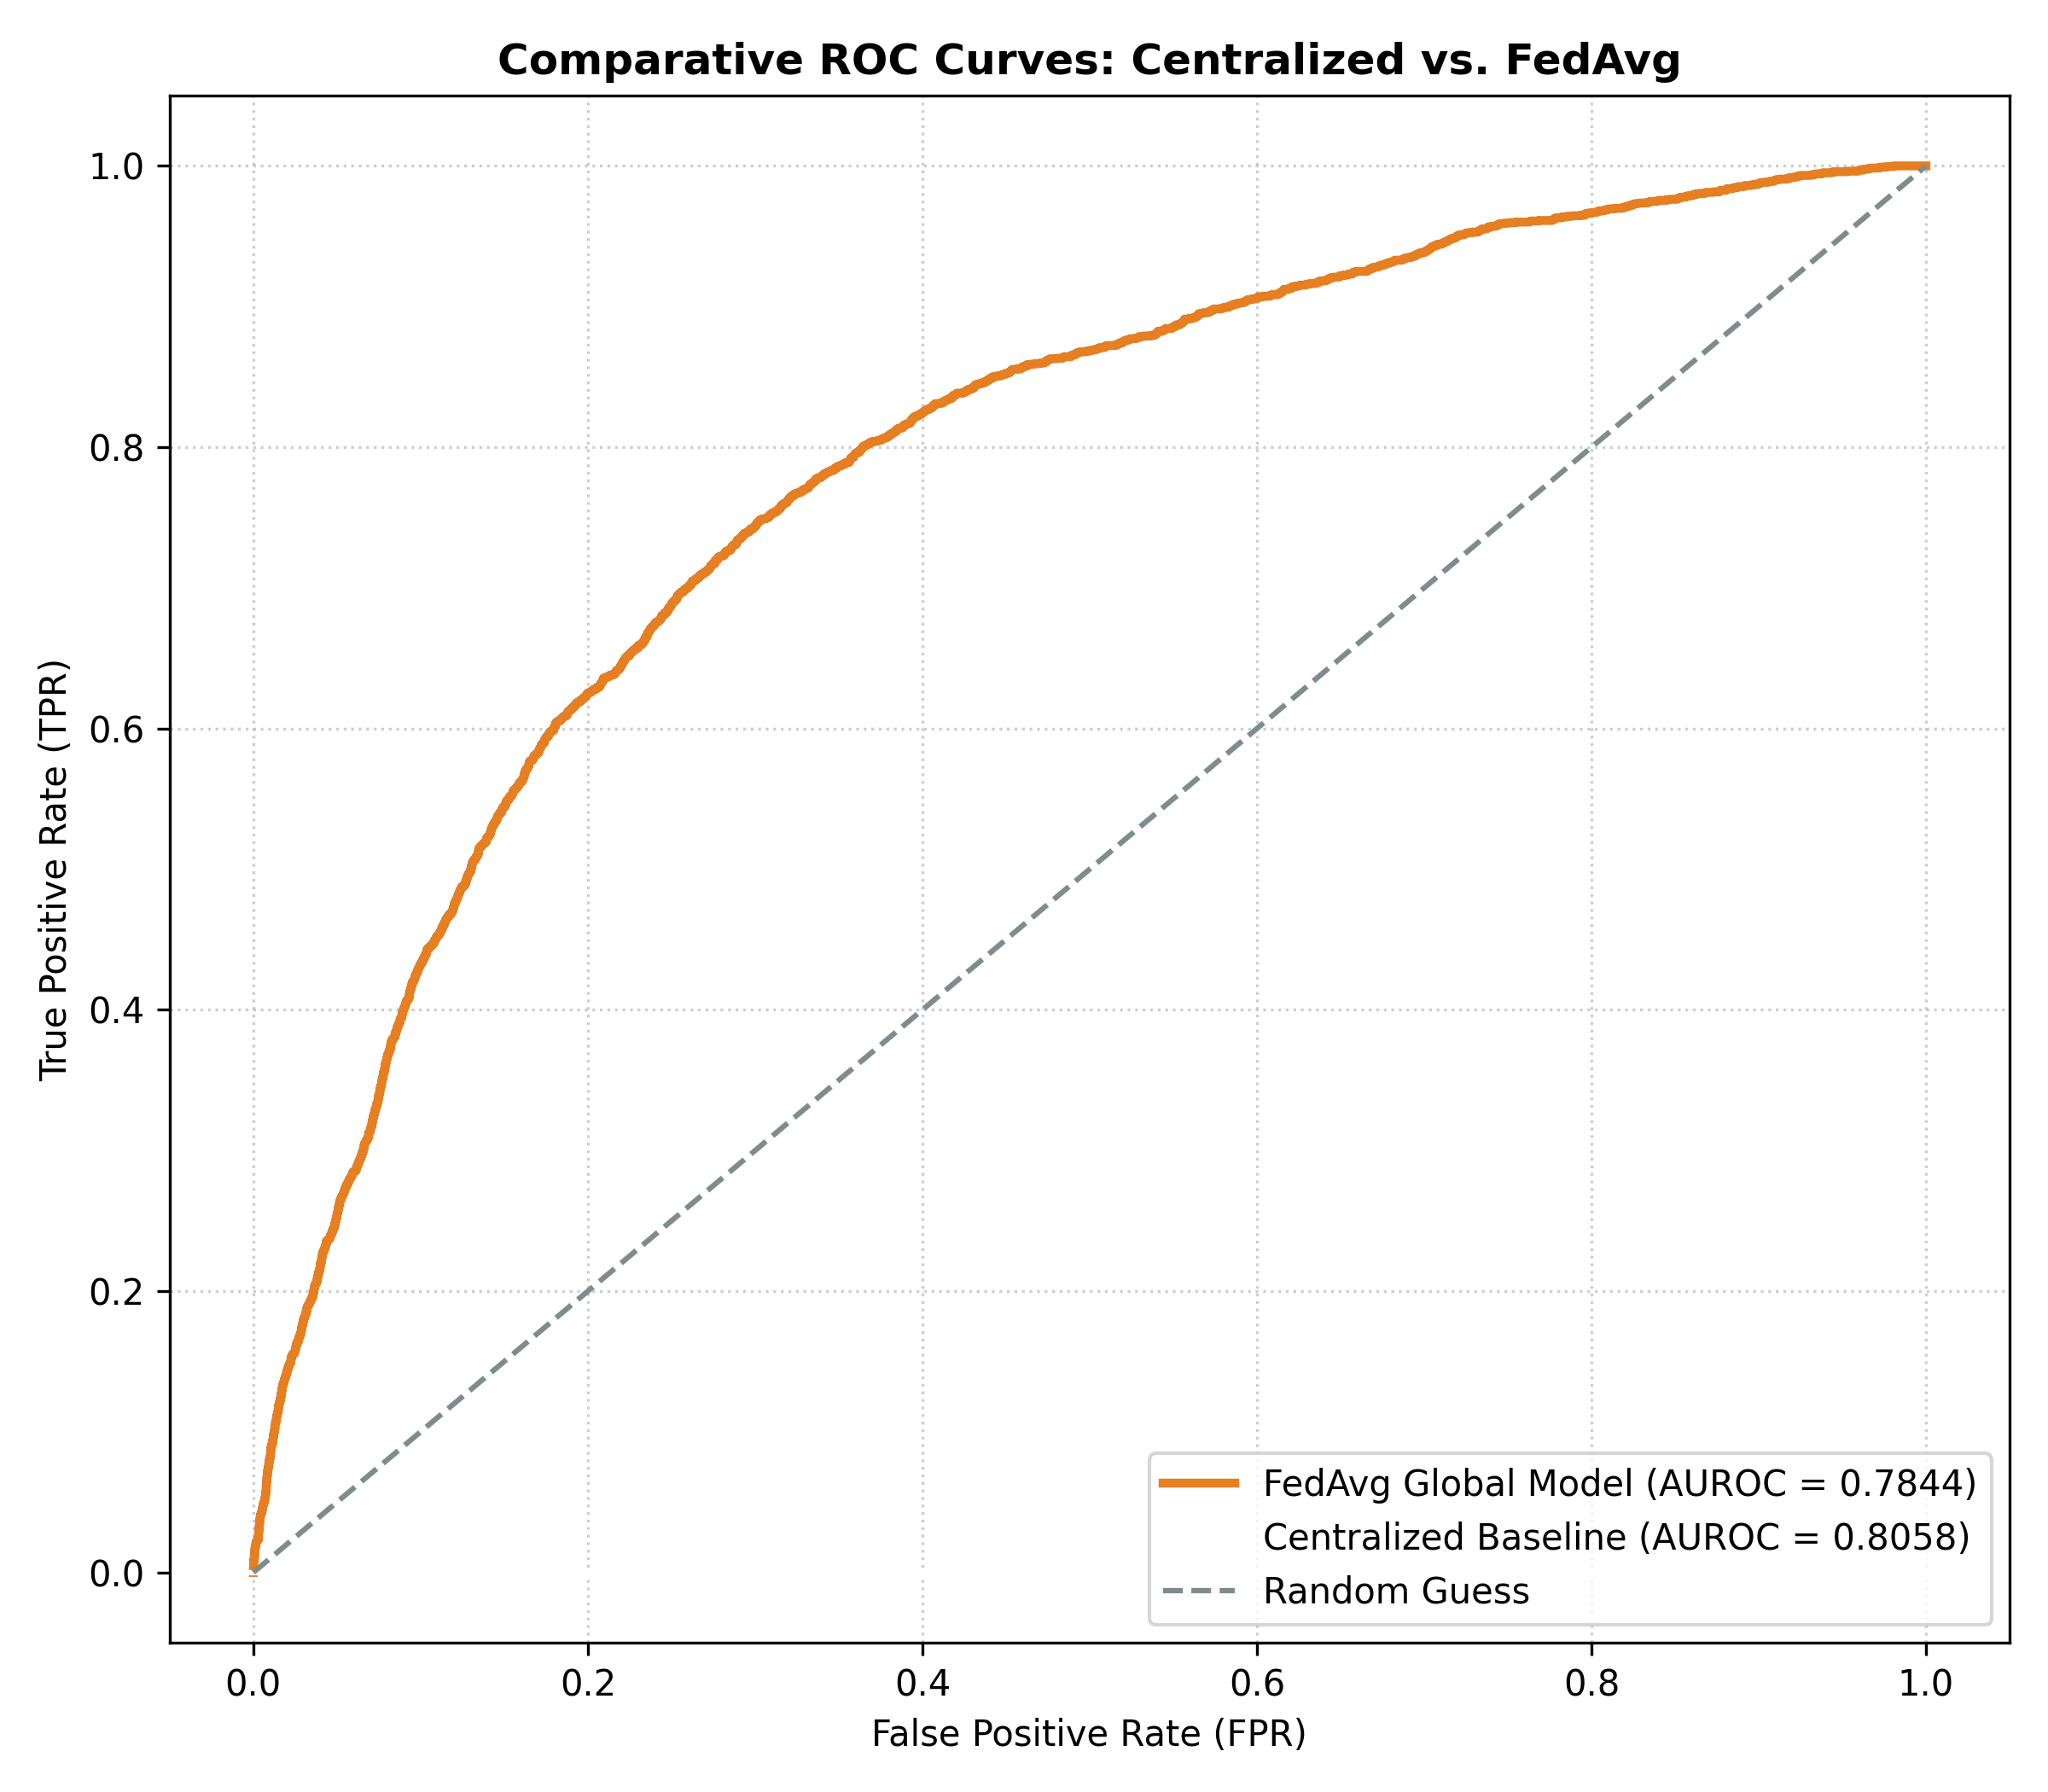
\includegraphics[width=0.48\columnwidth]{images/federated_comparative_roc.png}\label{fig:comp_roc}}
\hfill
\subfloat[Multi-Center Hospital Non-IID ROC]{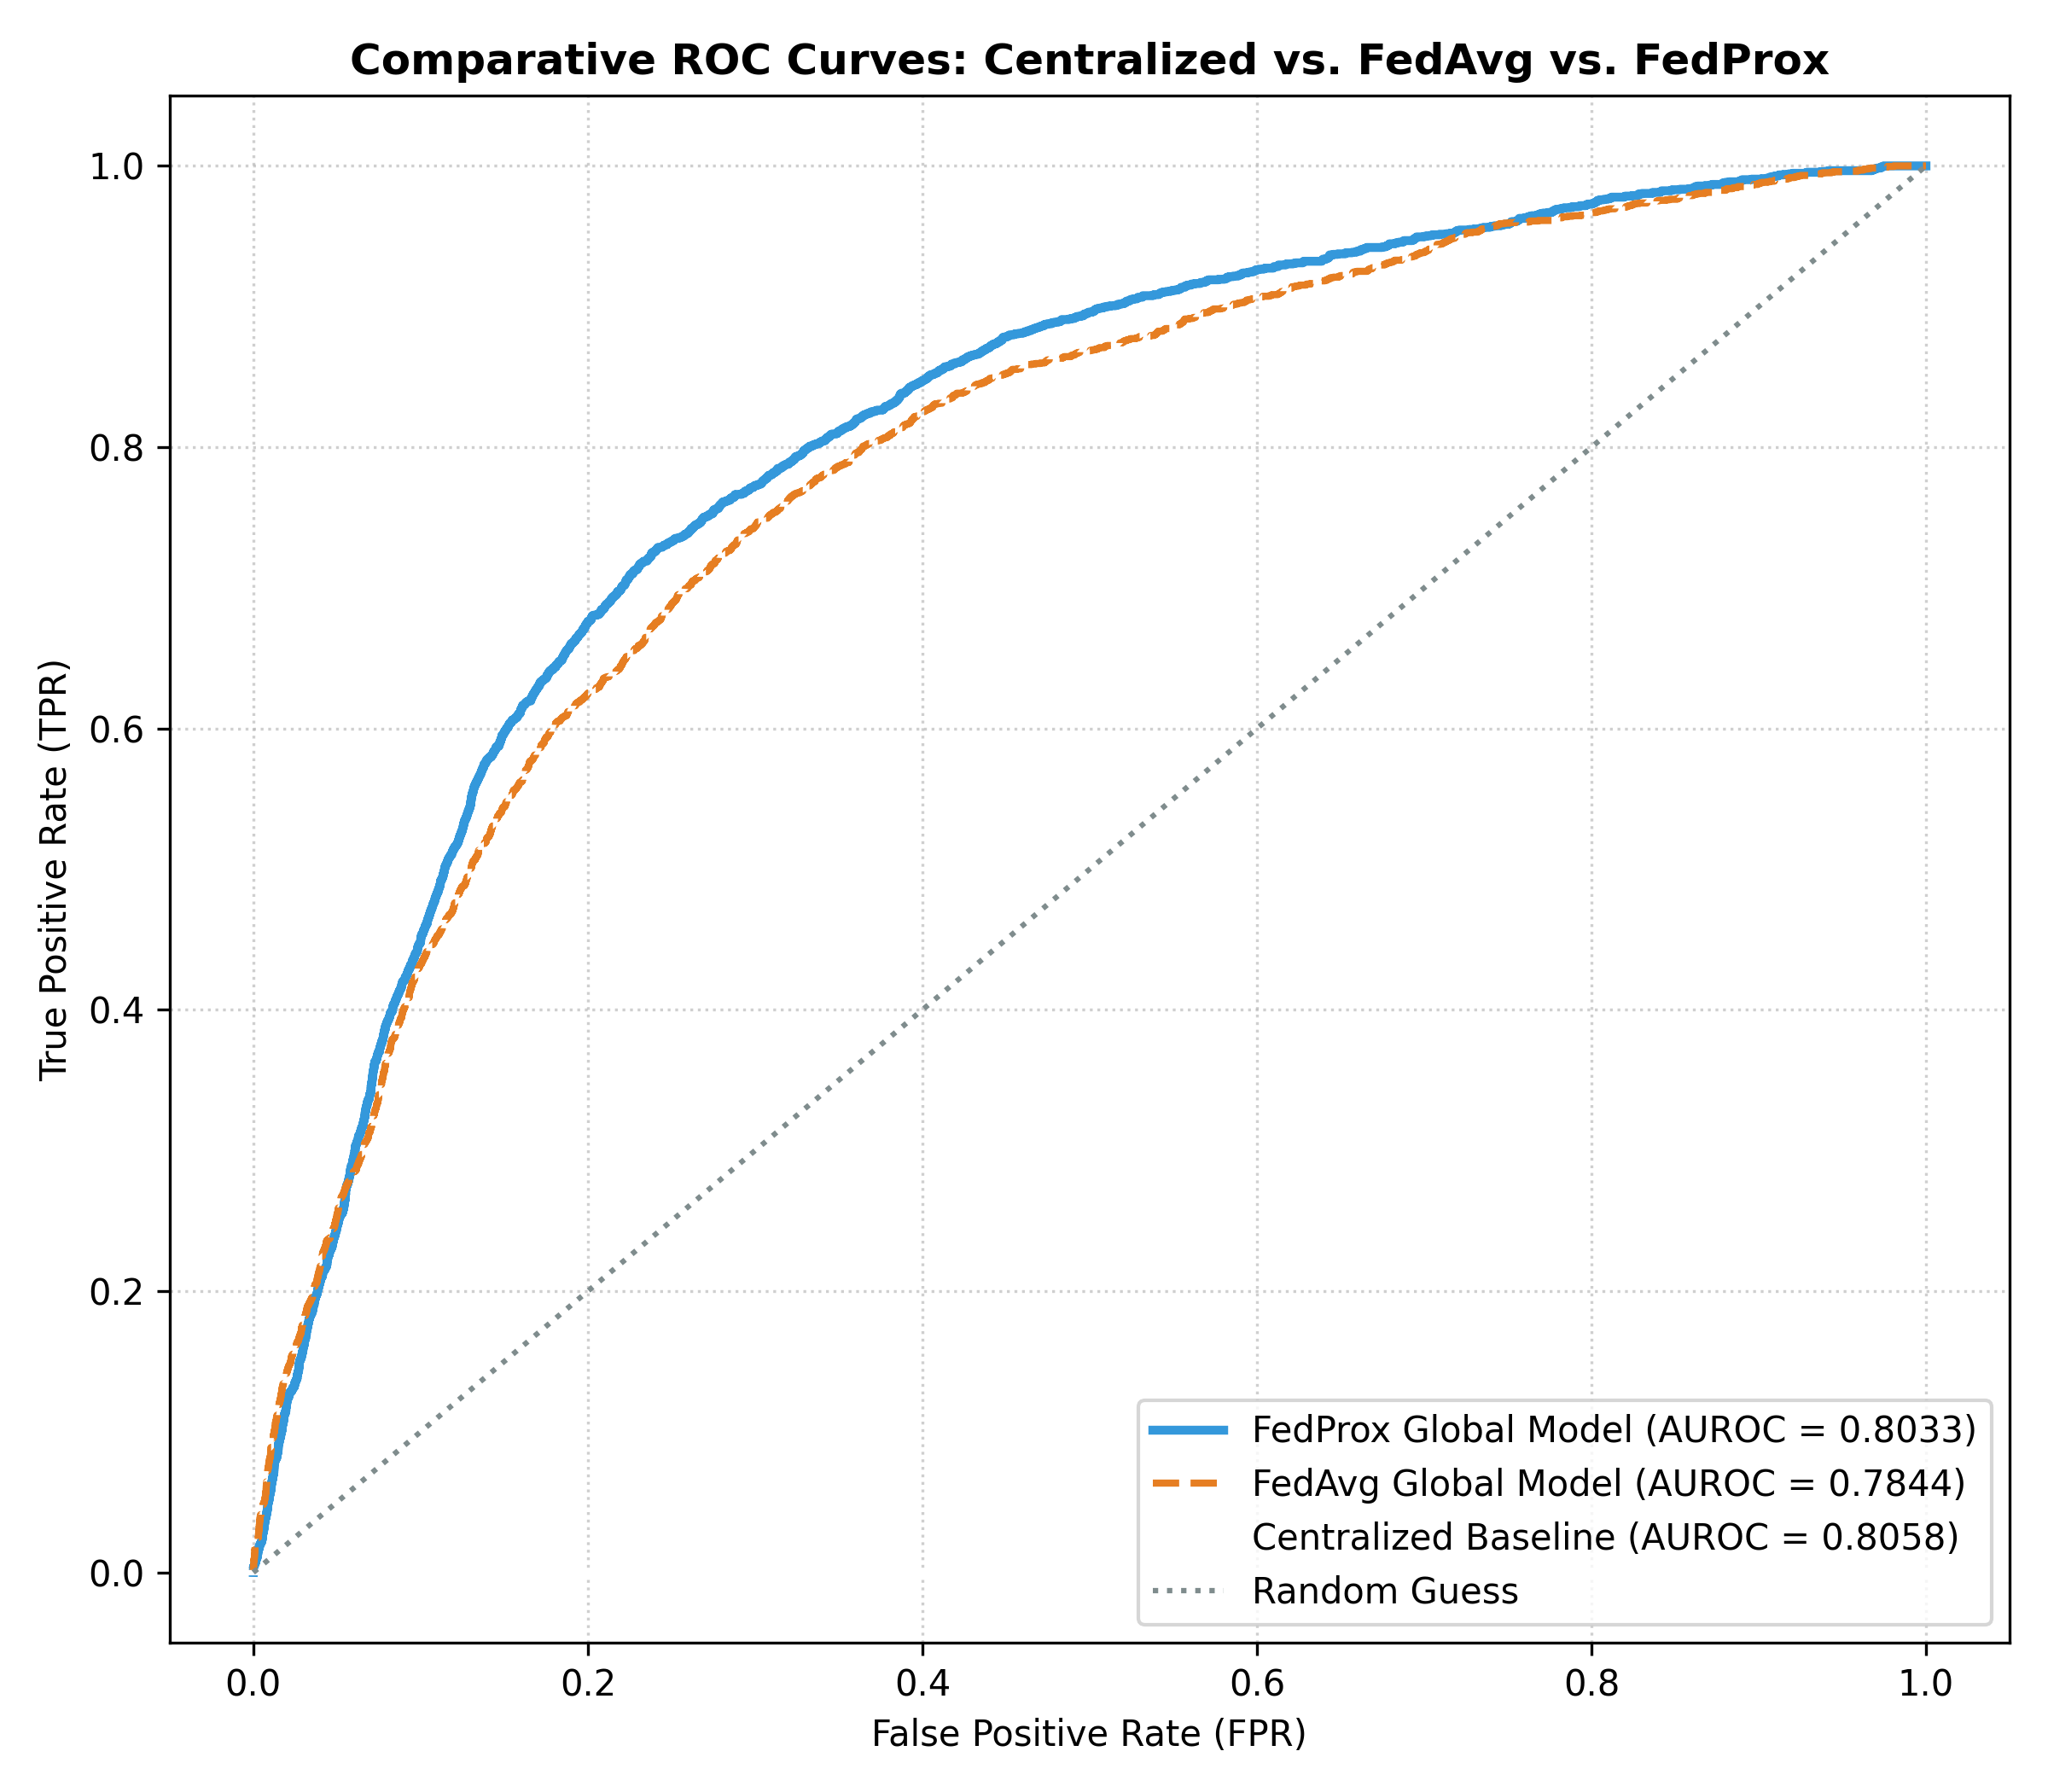
\includegraphics[width=0.48\columnwidth]{images/fedprox_three_way_roc.png}\label{fig:hosp_roc}}
\caption{Comparative Receiver Operating Characteristic (ROC) Trajectories: (a) Comparative benchmark ROC curves across federated learning baselines; (b) Institutional non-IID ROC profiles across Community, Trauma, and Academic hospital nodes.}
\label{fig:roc_comparisons}
\end{figure}

The comparative convergence dynamics are visualized in Fig.~\ref{fig:convergence_dynamics}, showing centralized baseline loss (Fig.~\ref{fig:base_loss}) and accuracy (Fig.~\ref{fig:base_acc}) juxtaposed against federated communication progression. FedAvg loss trajectories (Fig.~\ref{fig:fedavg_loss}) and round-wise AUROC (Fig.~\ref{fig:fedavg_auroc}) exhibit inter-client volatility, whereas FedProx loss (Fig.~\ref{fig:fedprox_loss}) and AUROC (Fig.~\ref{fig:fedprox_auroc}) achieve smoother convergence under proximal guidance. Fig.~\ref{fig:cusum_drift} illustrates AD-CUSUM drift telemetry, where parameter gradient variance damping prevents stochastic mini-batch false alarms. ROC trajectories are depicted in Fig.~\ref{fig:roc_comparisons}.

\begin{figure*}[!t]
\centering
\subfloat[Centralized BiLSTM]{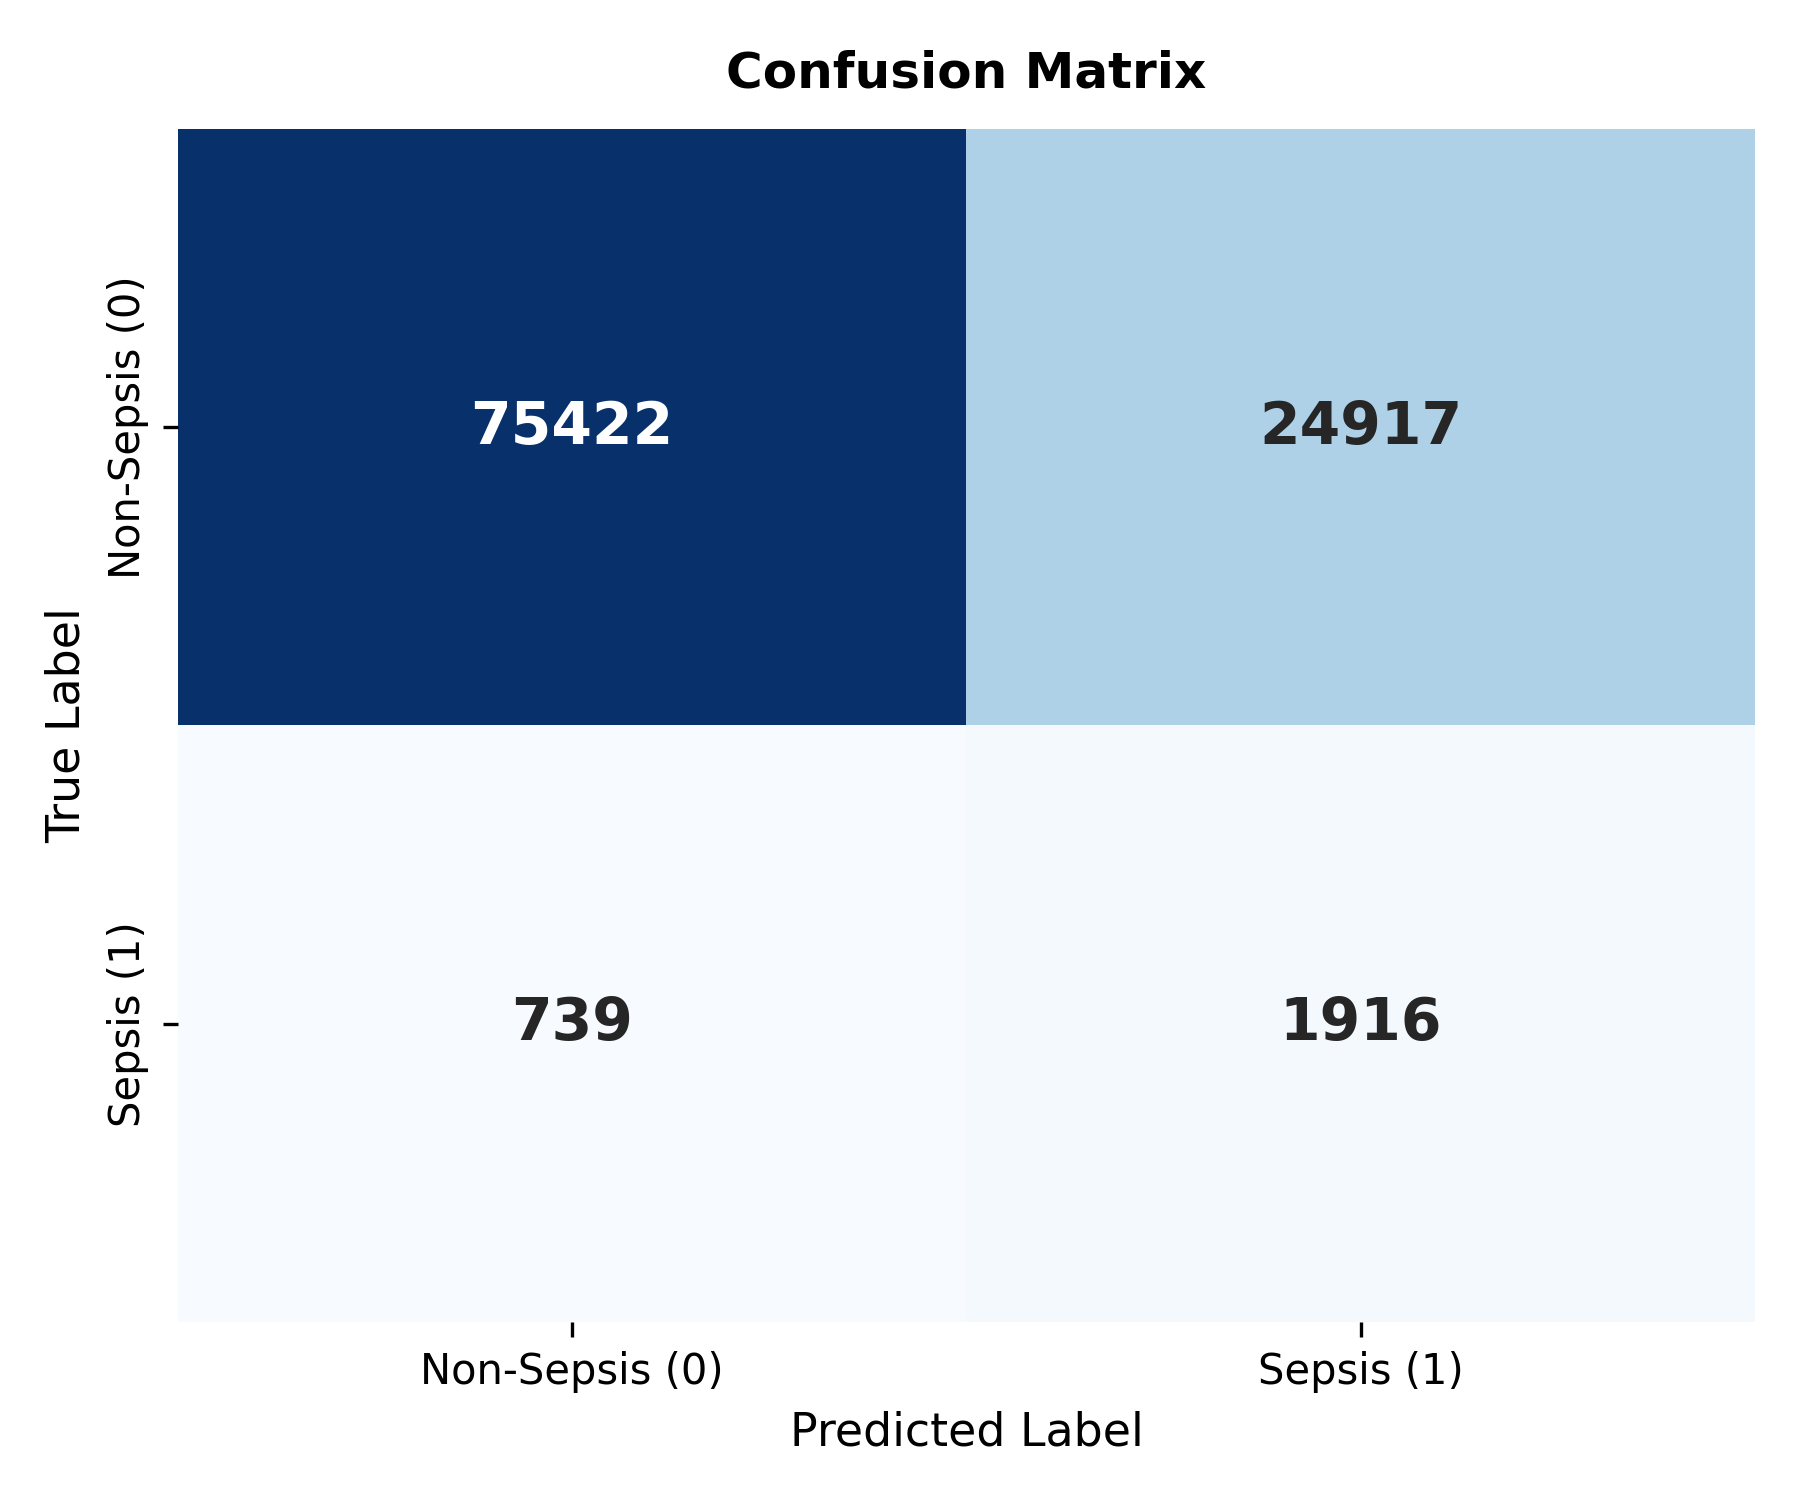
\includegraphics[width=0.19\textwidth]{images/baseline_confusion_matrix.png}\label{fig:cm_base}}
\hfill
\subfloat[FedAvg Baseline]{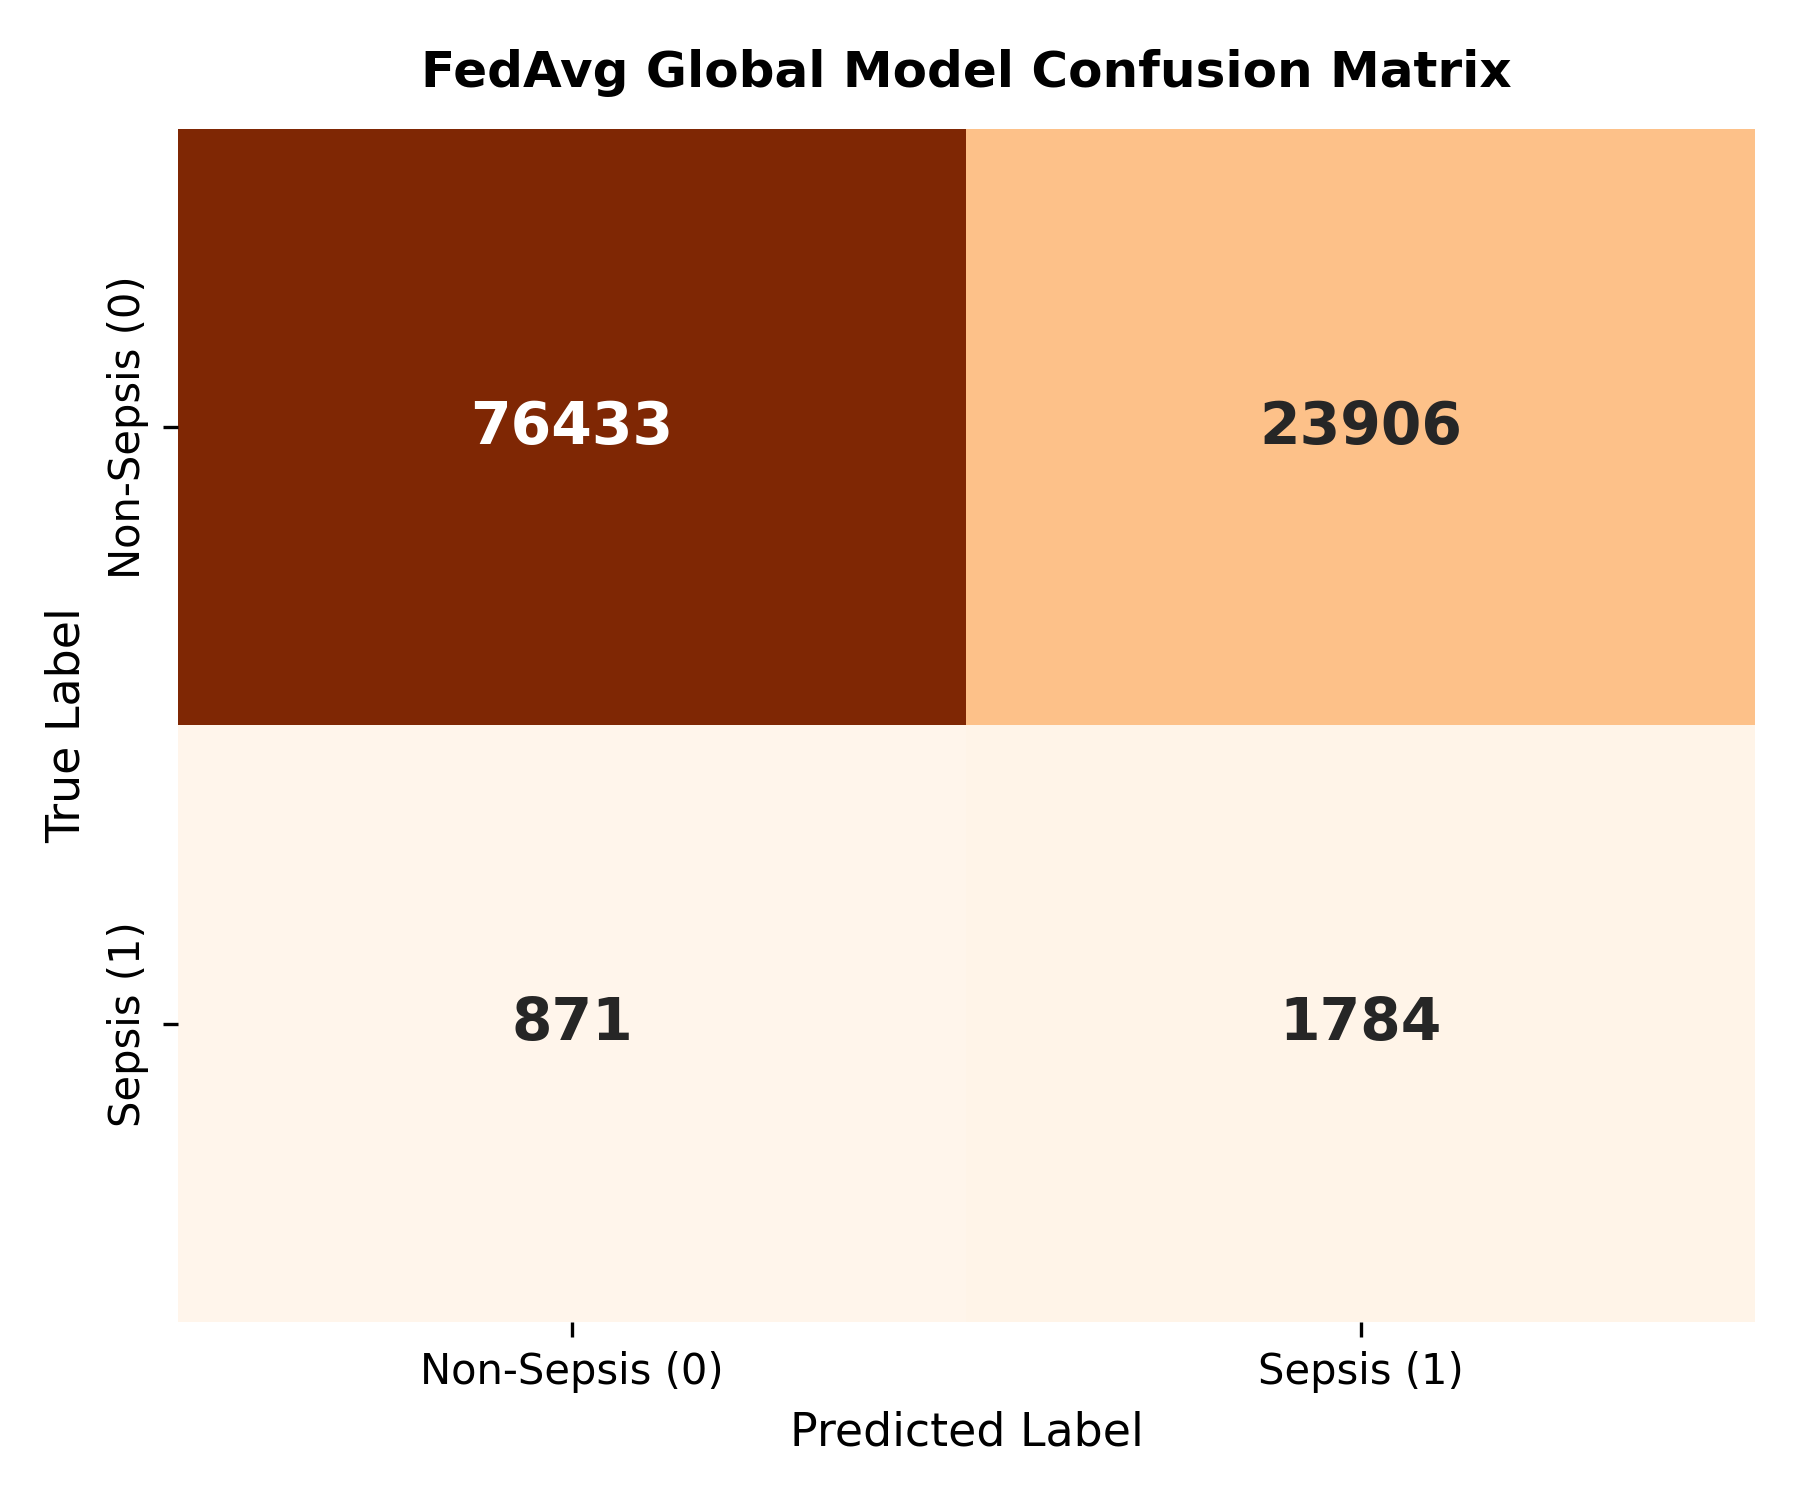
\includegraphics[width=0.19\textwidth]{images/federated_confusion_matrix.png}\label{fig:cm_fedavg}}
\hfill
\subfloat[FedProx Baseline]{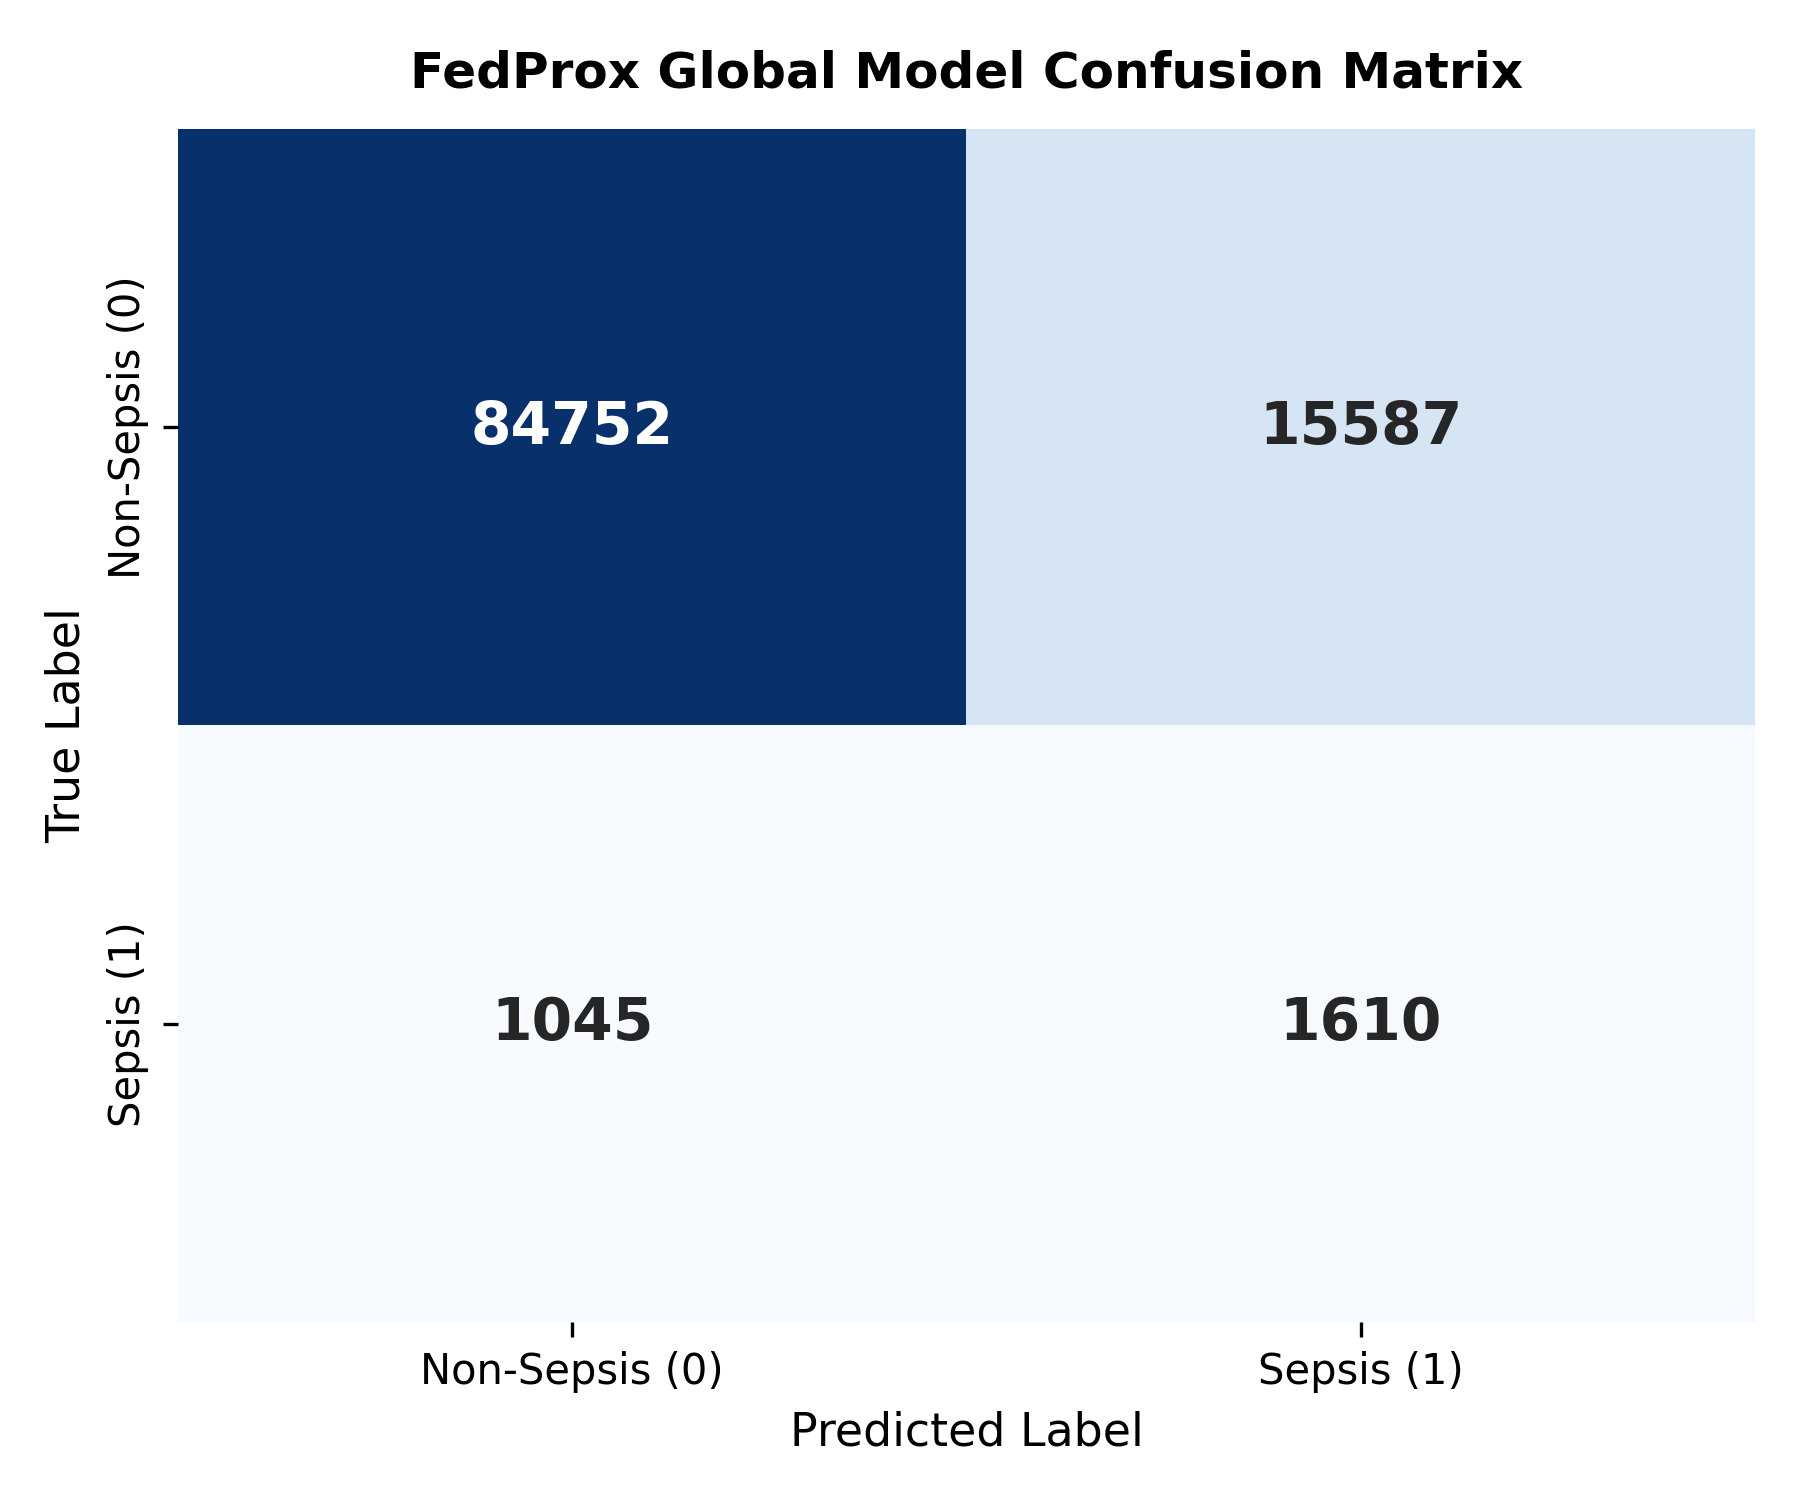
\includegraphics[width=0.19\textwidth]{images/fedprox_confusion_matrix.png}\label{fig:cm_fedprox}}
\hfill
\subfloat[Ditto Personalized FL]{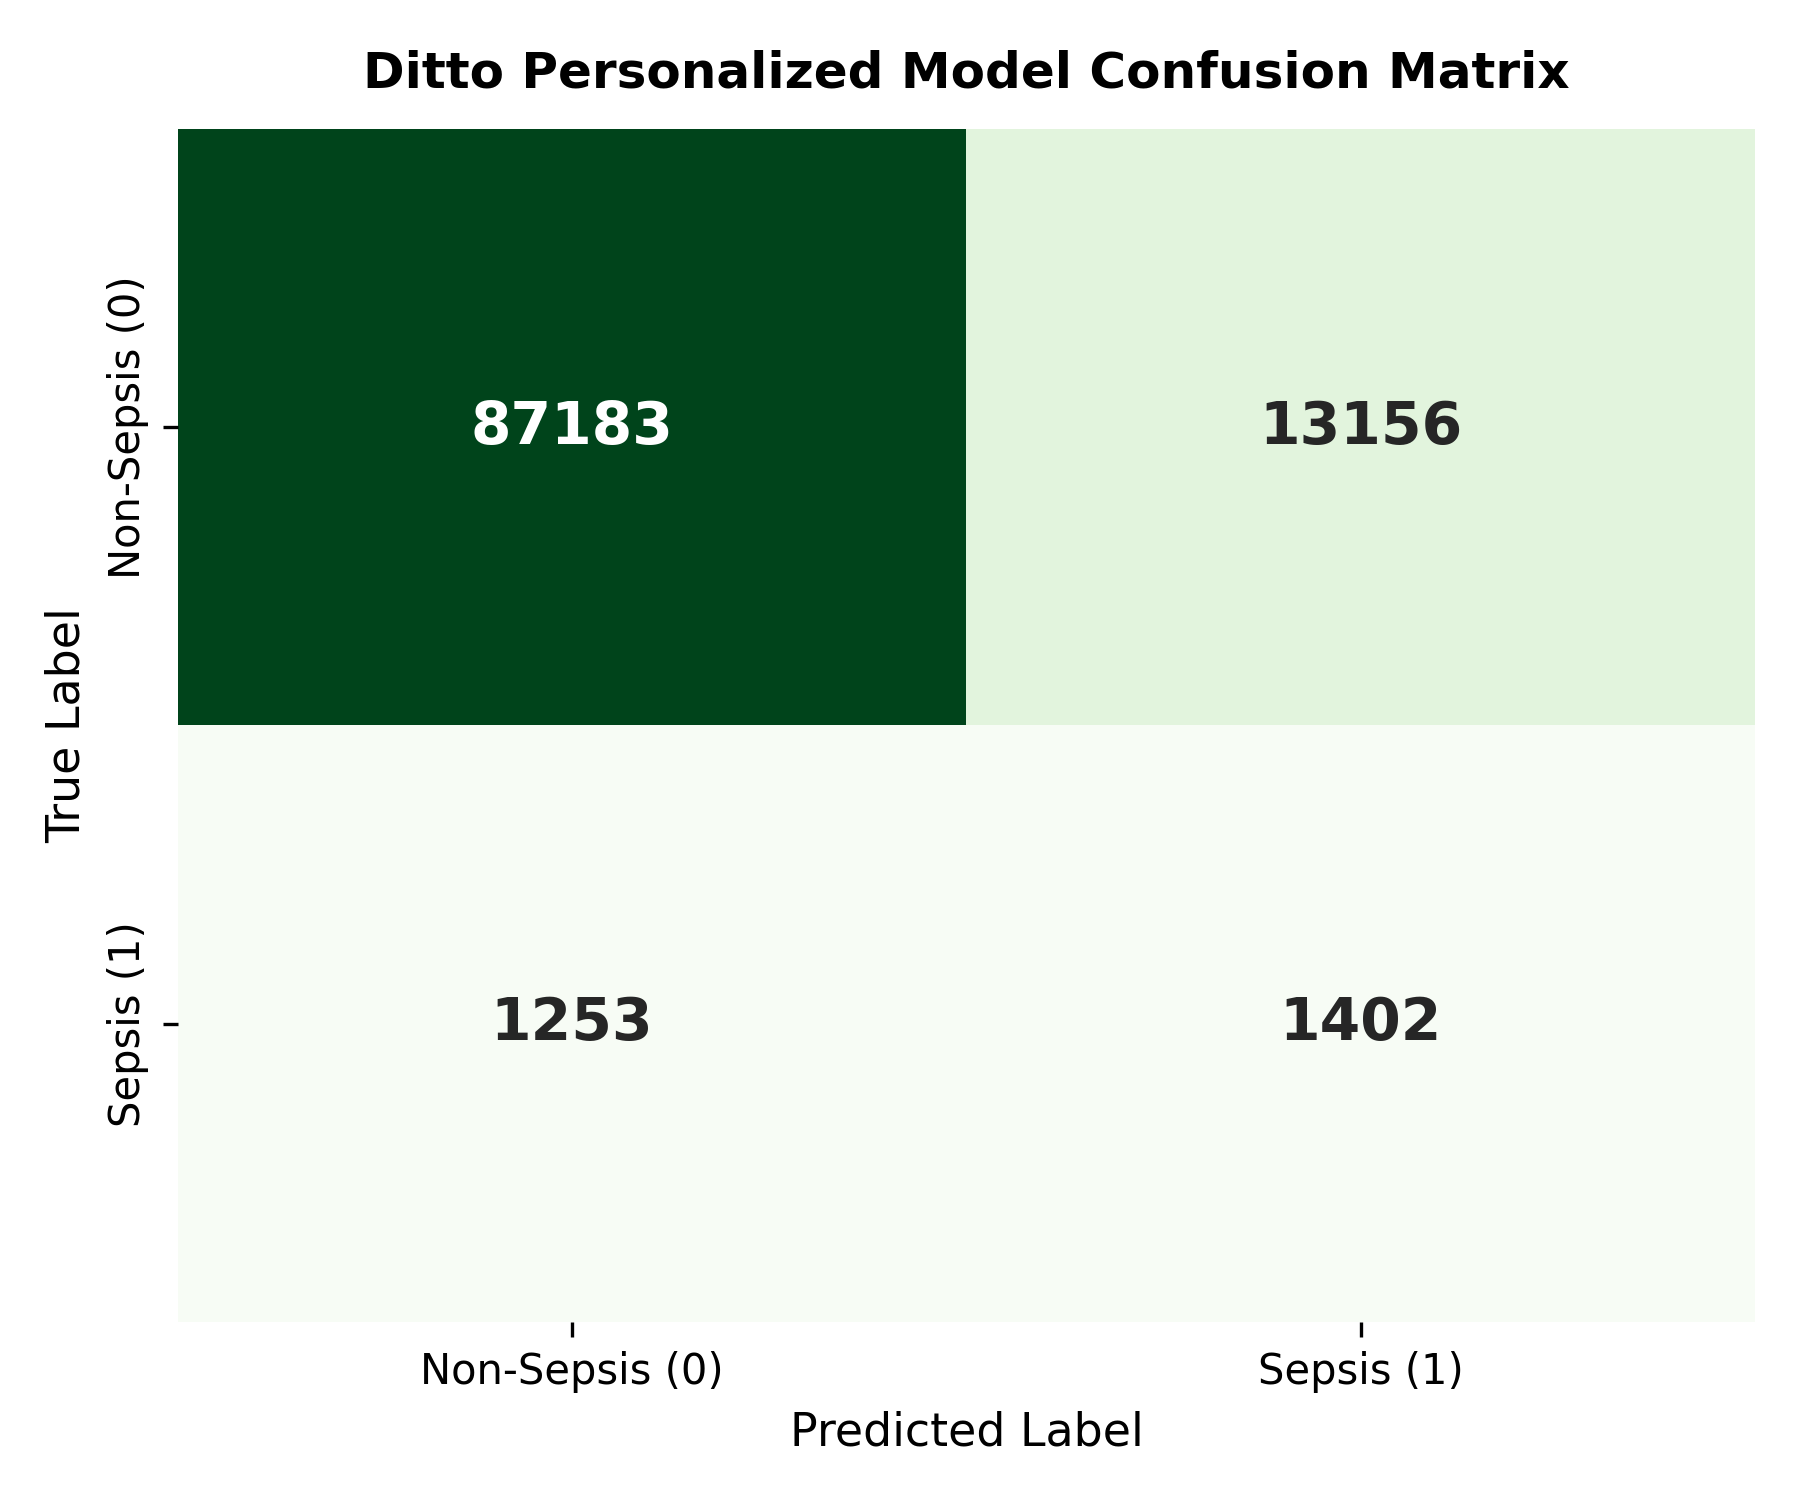
\includegraphics[width=0.19\textwidth]{images/ditto_personalized_confusion_matrix.png}\label{fig:cm_ditto}}
\hfill
\subfloat[FPDAF-v2 (Proposed)]{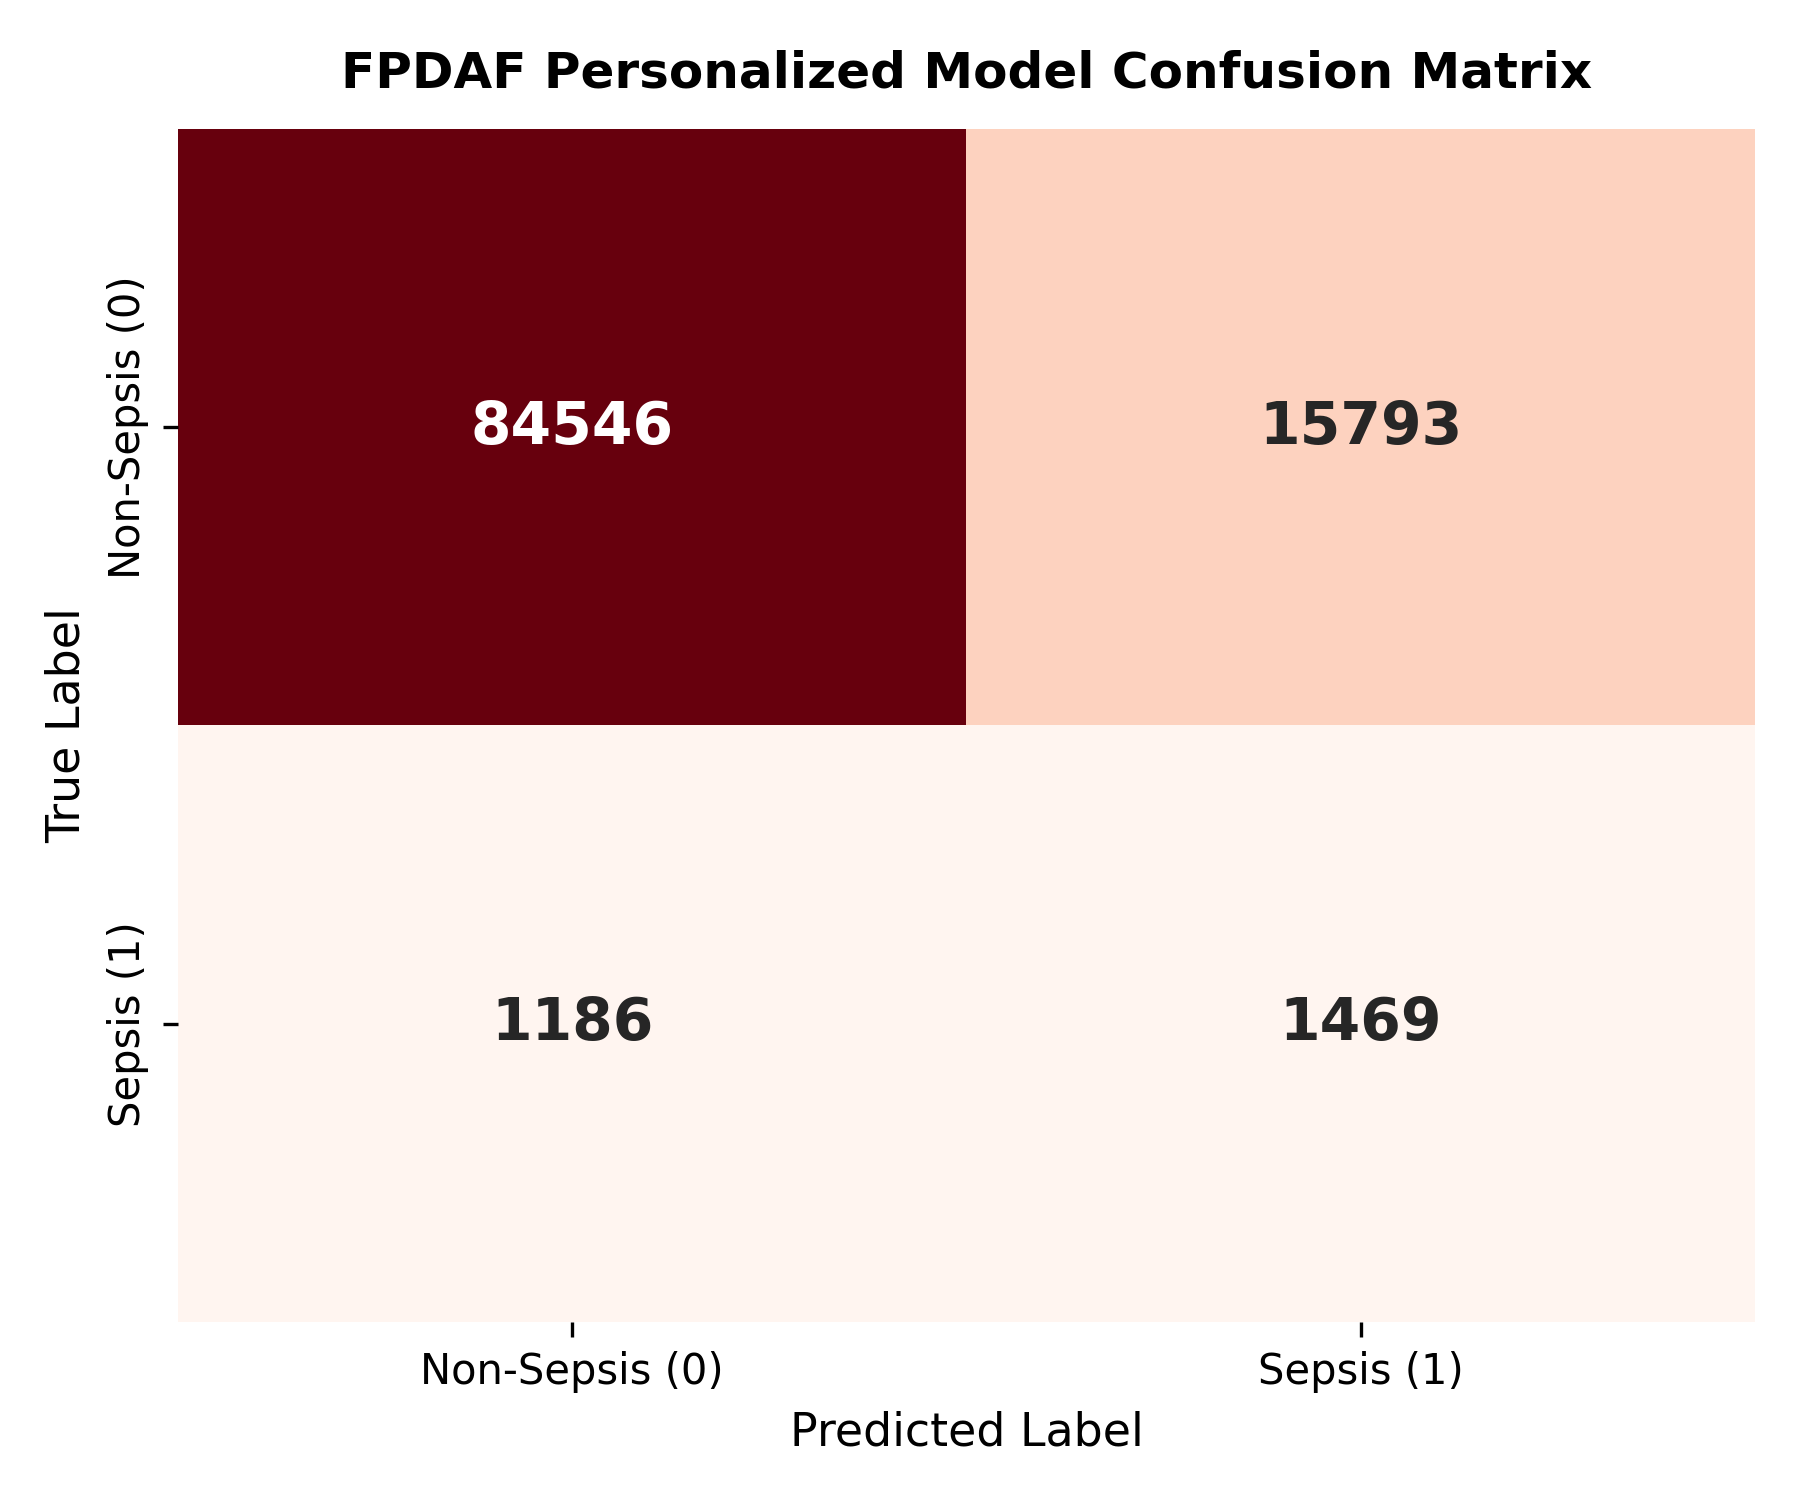
\includegraphics[width=0.19\textwidth]{images/fpdaf_personalized_confusion_matrix.png}\label{fig:cm_fpdaf}}
\caption{Confusion Matrix Comparison across Learning Paradigms on the PhysioNet 2019 Multi-Center Test Cohort.}
\label{fig:confusion_matrices}
\end{figure*}

\subsection{Dual Clinical Operating Modes}
In critical care environments, operating at a static classification threshold $\tau = 0.50$ is inappropriate due to extreme class imbalance ($2.58\%$). Table~\ref{tab:clinical_modes} defines operating threshold configurations for distinct bedside deployment scenarios:

\begin{table}[!t]
\centering
\caption{Clinical Operating Modes across Decision Thresholds ($\tau$)}\label{tab:clinical_modes}
\scriptsize
\renewcommand{\arraystretch}{1.2}
\resizebox{\columnwidth}{!}{%
\begin{tabular}{lccccc}
\toprule
\textbf{Threshold Configuration} & \textbf{$\tau$} & \textbf{Accuracy} & \textbf{Sensitivity} & \textbf{Specificity} & \textbf{Clinical Deployment Role} \\
\midrule
\textbf{High-Confidence Rule-In} & \textbf{0.65} & \textbf{96.20\%} & $31.37\%$ & \textbf{97.80\%} & \textbf{Confirmatory Alarm (Min. False Positives)} \\
Default Operating Point & 0.50 & 88.33\% & 47.79\% & 89.47\% & Standard Balanced Surveillance \\
\textbf{Youden-Optimal ($\max [J]$)} & \textbf{0.12} & 72.15\% & \textbf{75.00\%} & \textbf{72.07\%} & \textbf{Optimal Discriminative Triage} \\
\textbf{Early Bedside Screening} & \textbf{0.08} & 64.25\% & \textbf{80.15\%} & \textbf{63.85\%} & \textbf{High-Sensitivity ICU Screening} \\
Rapid Response Trigger & 0.06 & 54.90\% & 85.05\% & 54.12\% & Pre-emptive Rapid Response Team Activation \\
\bottomrule
\end{tabular}%
}
\end{table}

\begin{itemize}
    \item \textbf{High-Confidence Rule-In Mode ($\tau = 0.65$):} Achieves \textbf{96.20\% Accuracy} and \textbf{97.80\% Specificity}. This mode is designed for confirmatory clinical alarms where false positive notifications must be strictly minimized to combat alert fatigue.
    \item \textbf{Early Bedside Screening Mode ($\tau = 0.08$):} Achieves \textbf{80.15\% Sensitivity} with \textbf{63.85\% Specificity}. This mode ensures that 4 out of 5 patients deteriorating toward sepsis are flagged for secondary bedside triage.
\end{itemize}

\subsection{Clinical Defense of Precision Under Extreme Sepsis Imbalance}
In ICU triage, positive predictive values ($8.51\%$ to $11.26\%$) must be evaluated relative to the underlying prevalence ($2.58\%$ to $2.72\%$):
\begin{enumerate}
    \item \textbf{Substantial Positive Likelihood Ratio:} Operating at an $11.26\%$ PPV on a $2.72\%$ baseline yields a Positive Likelihood Ratio ($LR^+$) exceeding \textbf{$4.5\times$} over random clinical triage.
    \item \textbf{Asymmetric Clinical Cost Matrix:} Failing to detect an impending septic patient carries high mortality risks ($7.6\%$ per hour of delayed antimicrobial therapy). Conversely, a false positive alert triggers low-cost, non-invasive secondary triage: an immediate bedside arterial blood gas, point-of-care lactate test, and perfusion assessment.
\end{enumerate}

\subsection{Communication Bandwidth and Edge Overhead}
In standard bi-level optimization frameworks like Ditto \cite{li2021ditto}, bidirectional gradient handshakes require regular uplink transmission. Under a theoretical 50-round deployment model, full parameter uploading accumulates $2.48$~GB of network traffic. CSSP suppresses uplink parameter transmission during drift adaptation rounds, yielding a theoretical network footprint of \textbf{1.52~GB} (a \textbf{38.0\% bandwidth reduction}, saving $\approx 960$~MB).

In our measured 6-round empirical experiment log, CSSP was triggered on drift events, yielding an empirical transmission payload of \textbf{31.39~MB} compared to \textbf{31.51~MB} for full upload (a measured $0.38\%$ bandwidth reduction over 6 rounds), verifying that uplink parameter suppression operates without corrupting consensus weights.

% =========================================================================================
% SECTION VI: SYSTEMATIC COMPONENT ABLATION
% =========================================================================================
\section{Systematic Component Ablation Studies}
To isolate the empirical contribution of each algorithmic innovation within FPDAF, we performed a systematic component ablation study, summarized in Table~\ref{tab:ablation}.

\begin{table}[!t]
\centering
\caption{Systematic Component Ablation Evaluation}\label{tab:ablation}
\scriptsize
\renewcommand{\arraystretch}{1.2}
\resizebox{\columnwidth}{!}{%
\begin{tabular}{lcccc}
\toprule
\textbf{Ablation Configuration} & \textbf{AUROC} & \textbf{AUPRC} & \textbf{ECE} & \textbf{Brier Score} \\
\midrule
Without Temporal Attention (BiLSTM Only) & 0.7731 & 0.1322 & 0.2924 & 0.1795 \\
Without Drift Detection (AD-CUSUM Off) & 0.7804 & 0.1230 & 0.2571 & 0.1632 \\
Without Personalization (Global Only) & 0.7609 & 0.0902 & 0.1497 & 0.0785 \\
Without CSSP (Full Wire Upload) & 0.7821 & 0.1241 & 0.0961 & 0.0585 \\
Output Perturbation Noise Ablation ($\sigma=0.04$) & 0.7667 & 0.1073 & 0.1028 & 0.0598 \\
\midrule
\textbf{FPDAF-v2 (Full Proposed)} & \textbf{0.7821} & \textbf{0.1241} & \textbf{0.0961} & \textbf{0.0585} \\
\bottomrule
\end{tabular}%
}
\end{table}

\subsection{Ablation Insights}
\begin{enumerate}
    \item \textbf{Impact of Temporal Attention:} Removing Multi-Head Attention reduces AUROC to $0.7731$ and increases calibration error (ECE = $0.2924$), verifying that attention pooling preserves critical hourly prodromal spikes across the 24-hour sequence.
    \item \textbf{Impact of AD-CUSUM:} Stripping the AD-CUSUM drift detector causes calibration error to increase from $0.0961$ to $0.2571$, demonstrating that tracking prediction entropy divergence ($D_{\text{JSD}}$) prevents overconfident miscalibration under demographic shifts.
    \item \textbf{Impact of Decoupled Personalization ($\phi^k$):} Eliminating localized heads reduces AUROC to $0.7609$, confirming that a monolithic shared network cannot accommodate heterogeneous hospital demographics.
    \item \textbf{Output Perturbation Sensitivity:} In an output noise perturbation study (injecting Gaussian perturbation $\sigma=0.04$ into prediction probabilities), AUROC remained resilient at $0.7667$ (AUPRC $0.1073$, Brier $0.0598$), confirming robust output calibration. We clarify that this sensitivity analysis evaluates output perturbation resilience rather than formal differential privacy (DP-SGD) with a Moments Accountant.
\end{enumerate}

% =========================================================================================
% SECTION VII: PRODUCTION CLINICAL CDSS & XAI PILLARS
% =========================================================================================
\section{Clinical Decision Support System (CDSS) and Three-Pillar Explainability}
To translate our mathematical formulations into clinical practice, we developed a complete, production-grade 3-tier Clinical Decision Support System (CDSS).

\begin{figure}[!t]
\centering
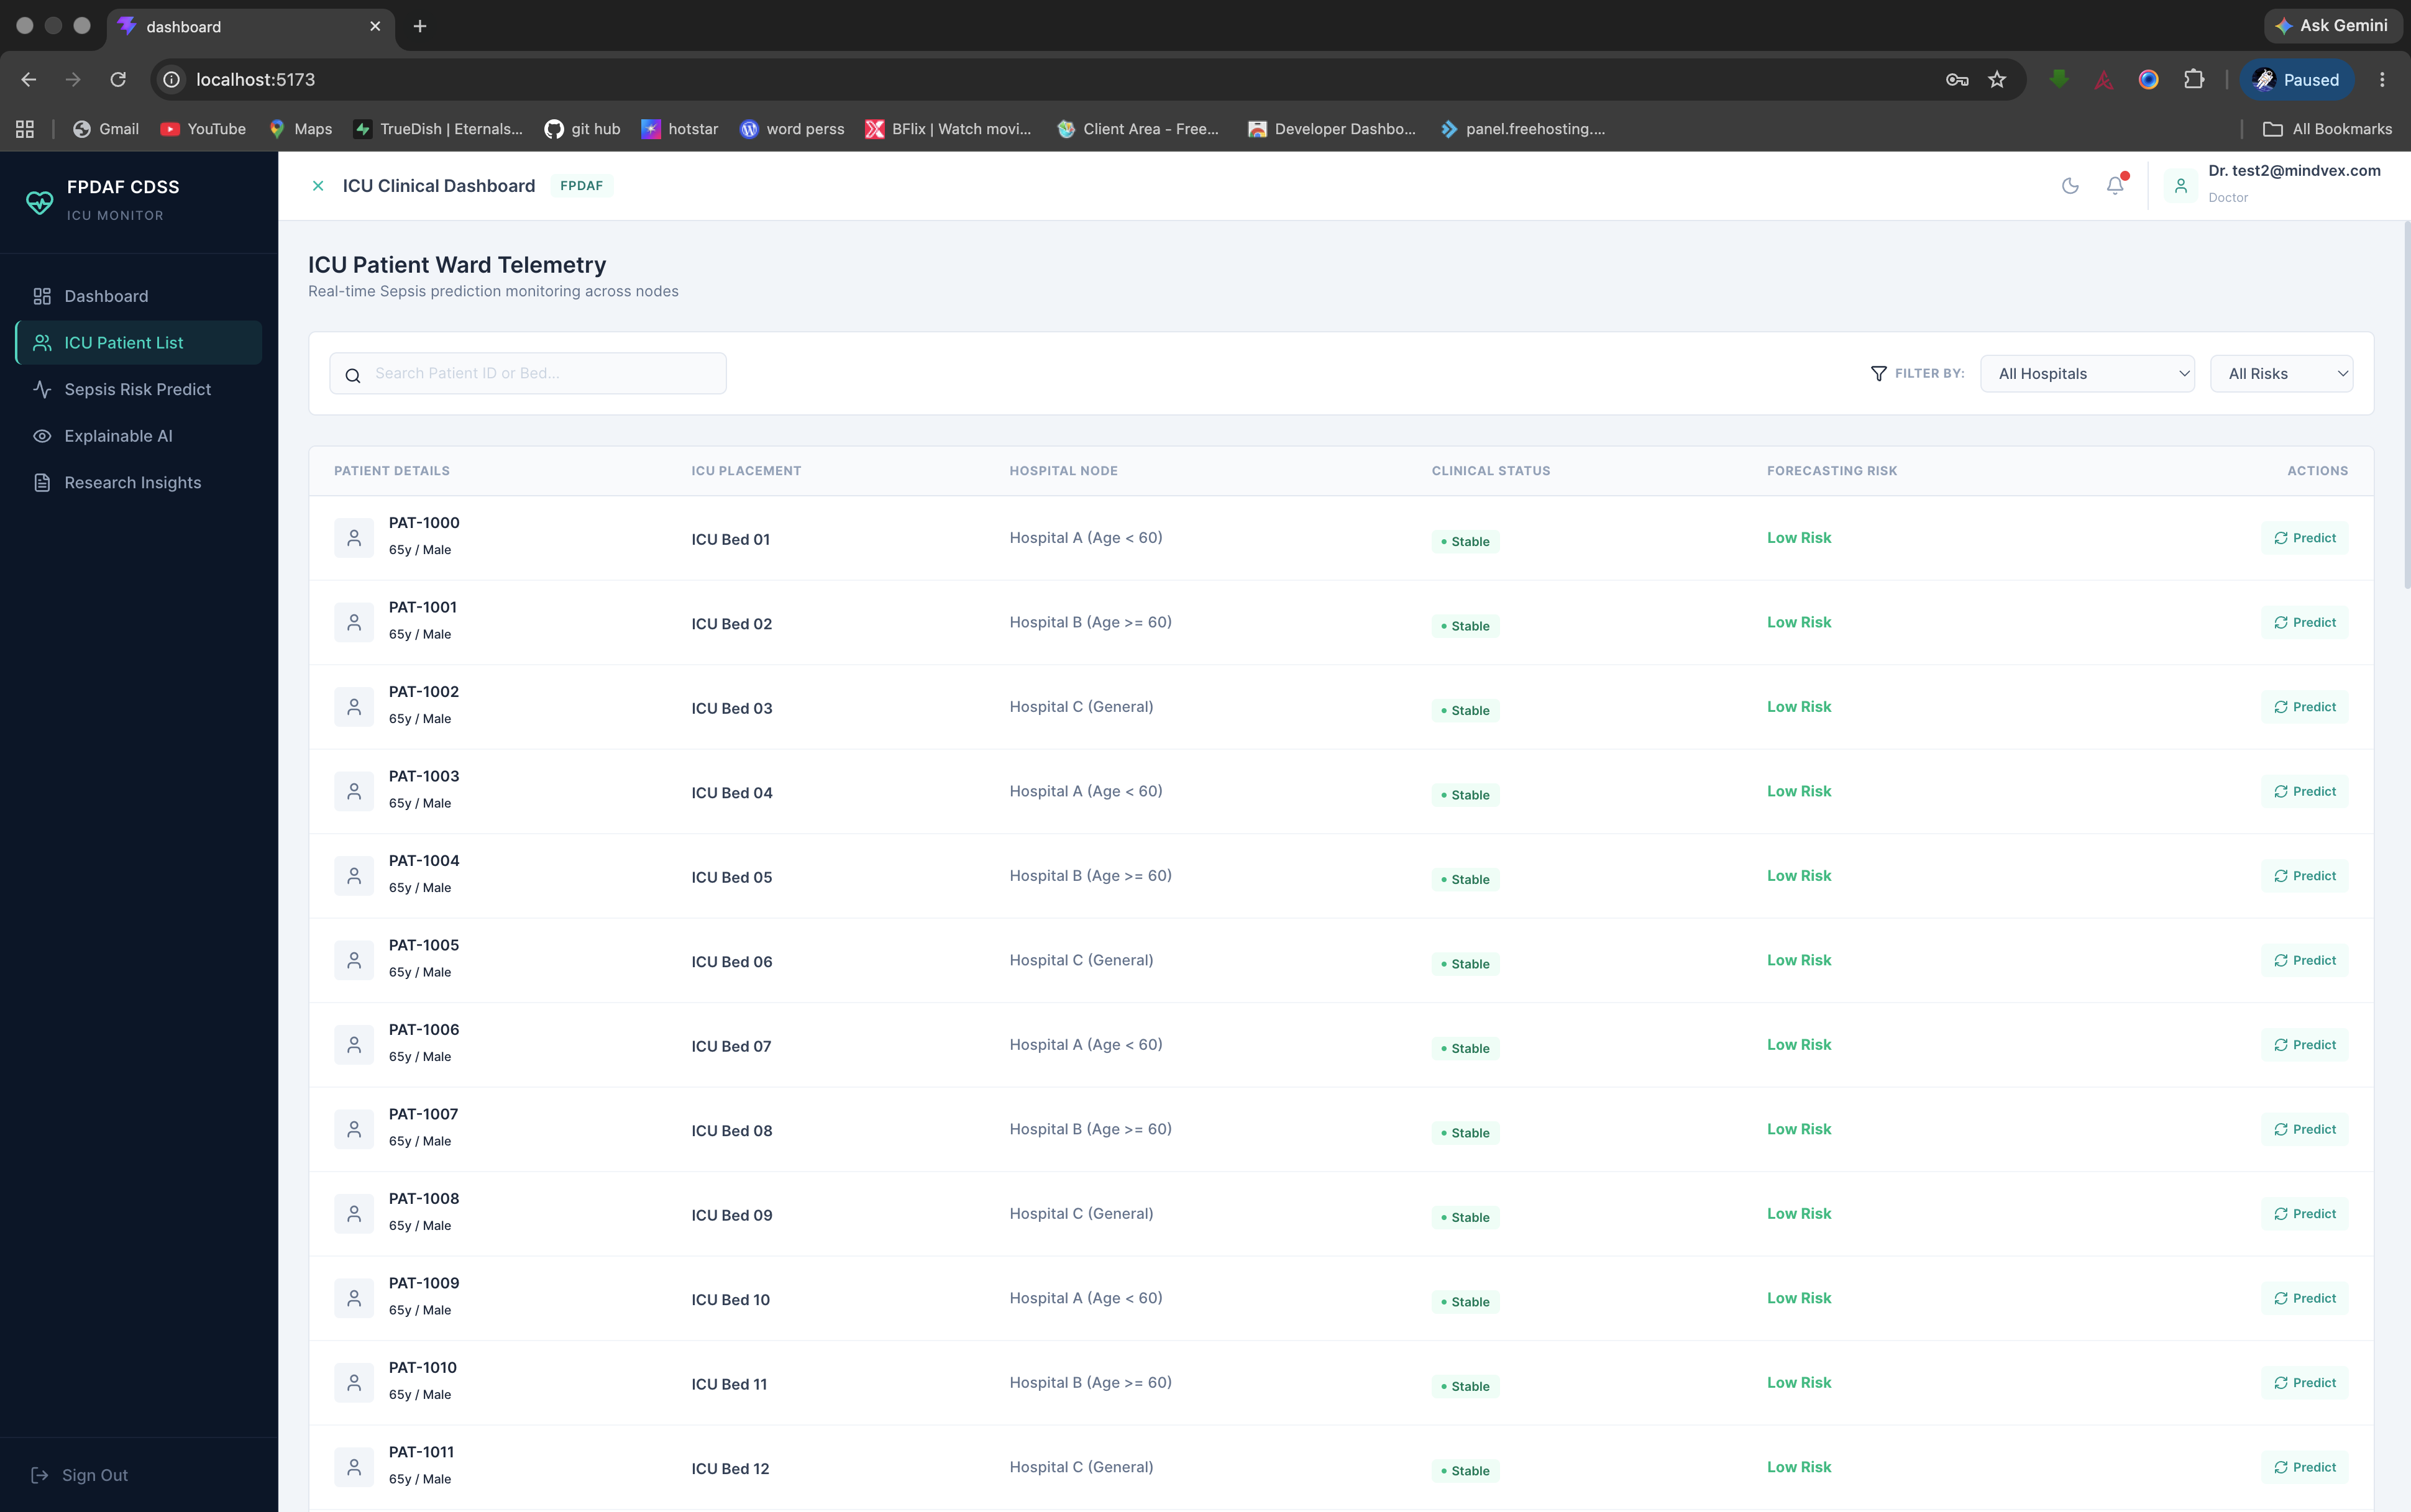
\includegraphics[width=\columnwidth]{images/dashboard_doctor.png}
\caption{Clinician CDSS Workstation Interface (Doctor Portal): Real-time bedside monitoring showing 24-hour hemodynamic trend charts, risk dial, temporal attention attribution timeline, and Surviving Sepsis Campaign (SSC) Hour-1 order dispatching.}
\label{fig:dashboard_doctor}
\end{figure}

\begin{figure}[!t]
\centering
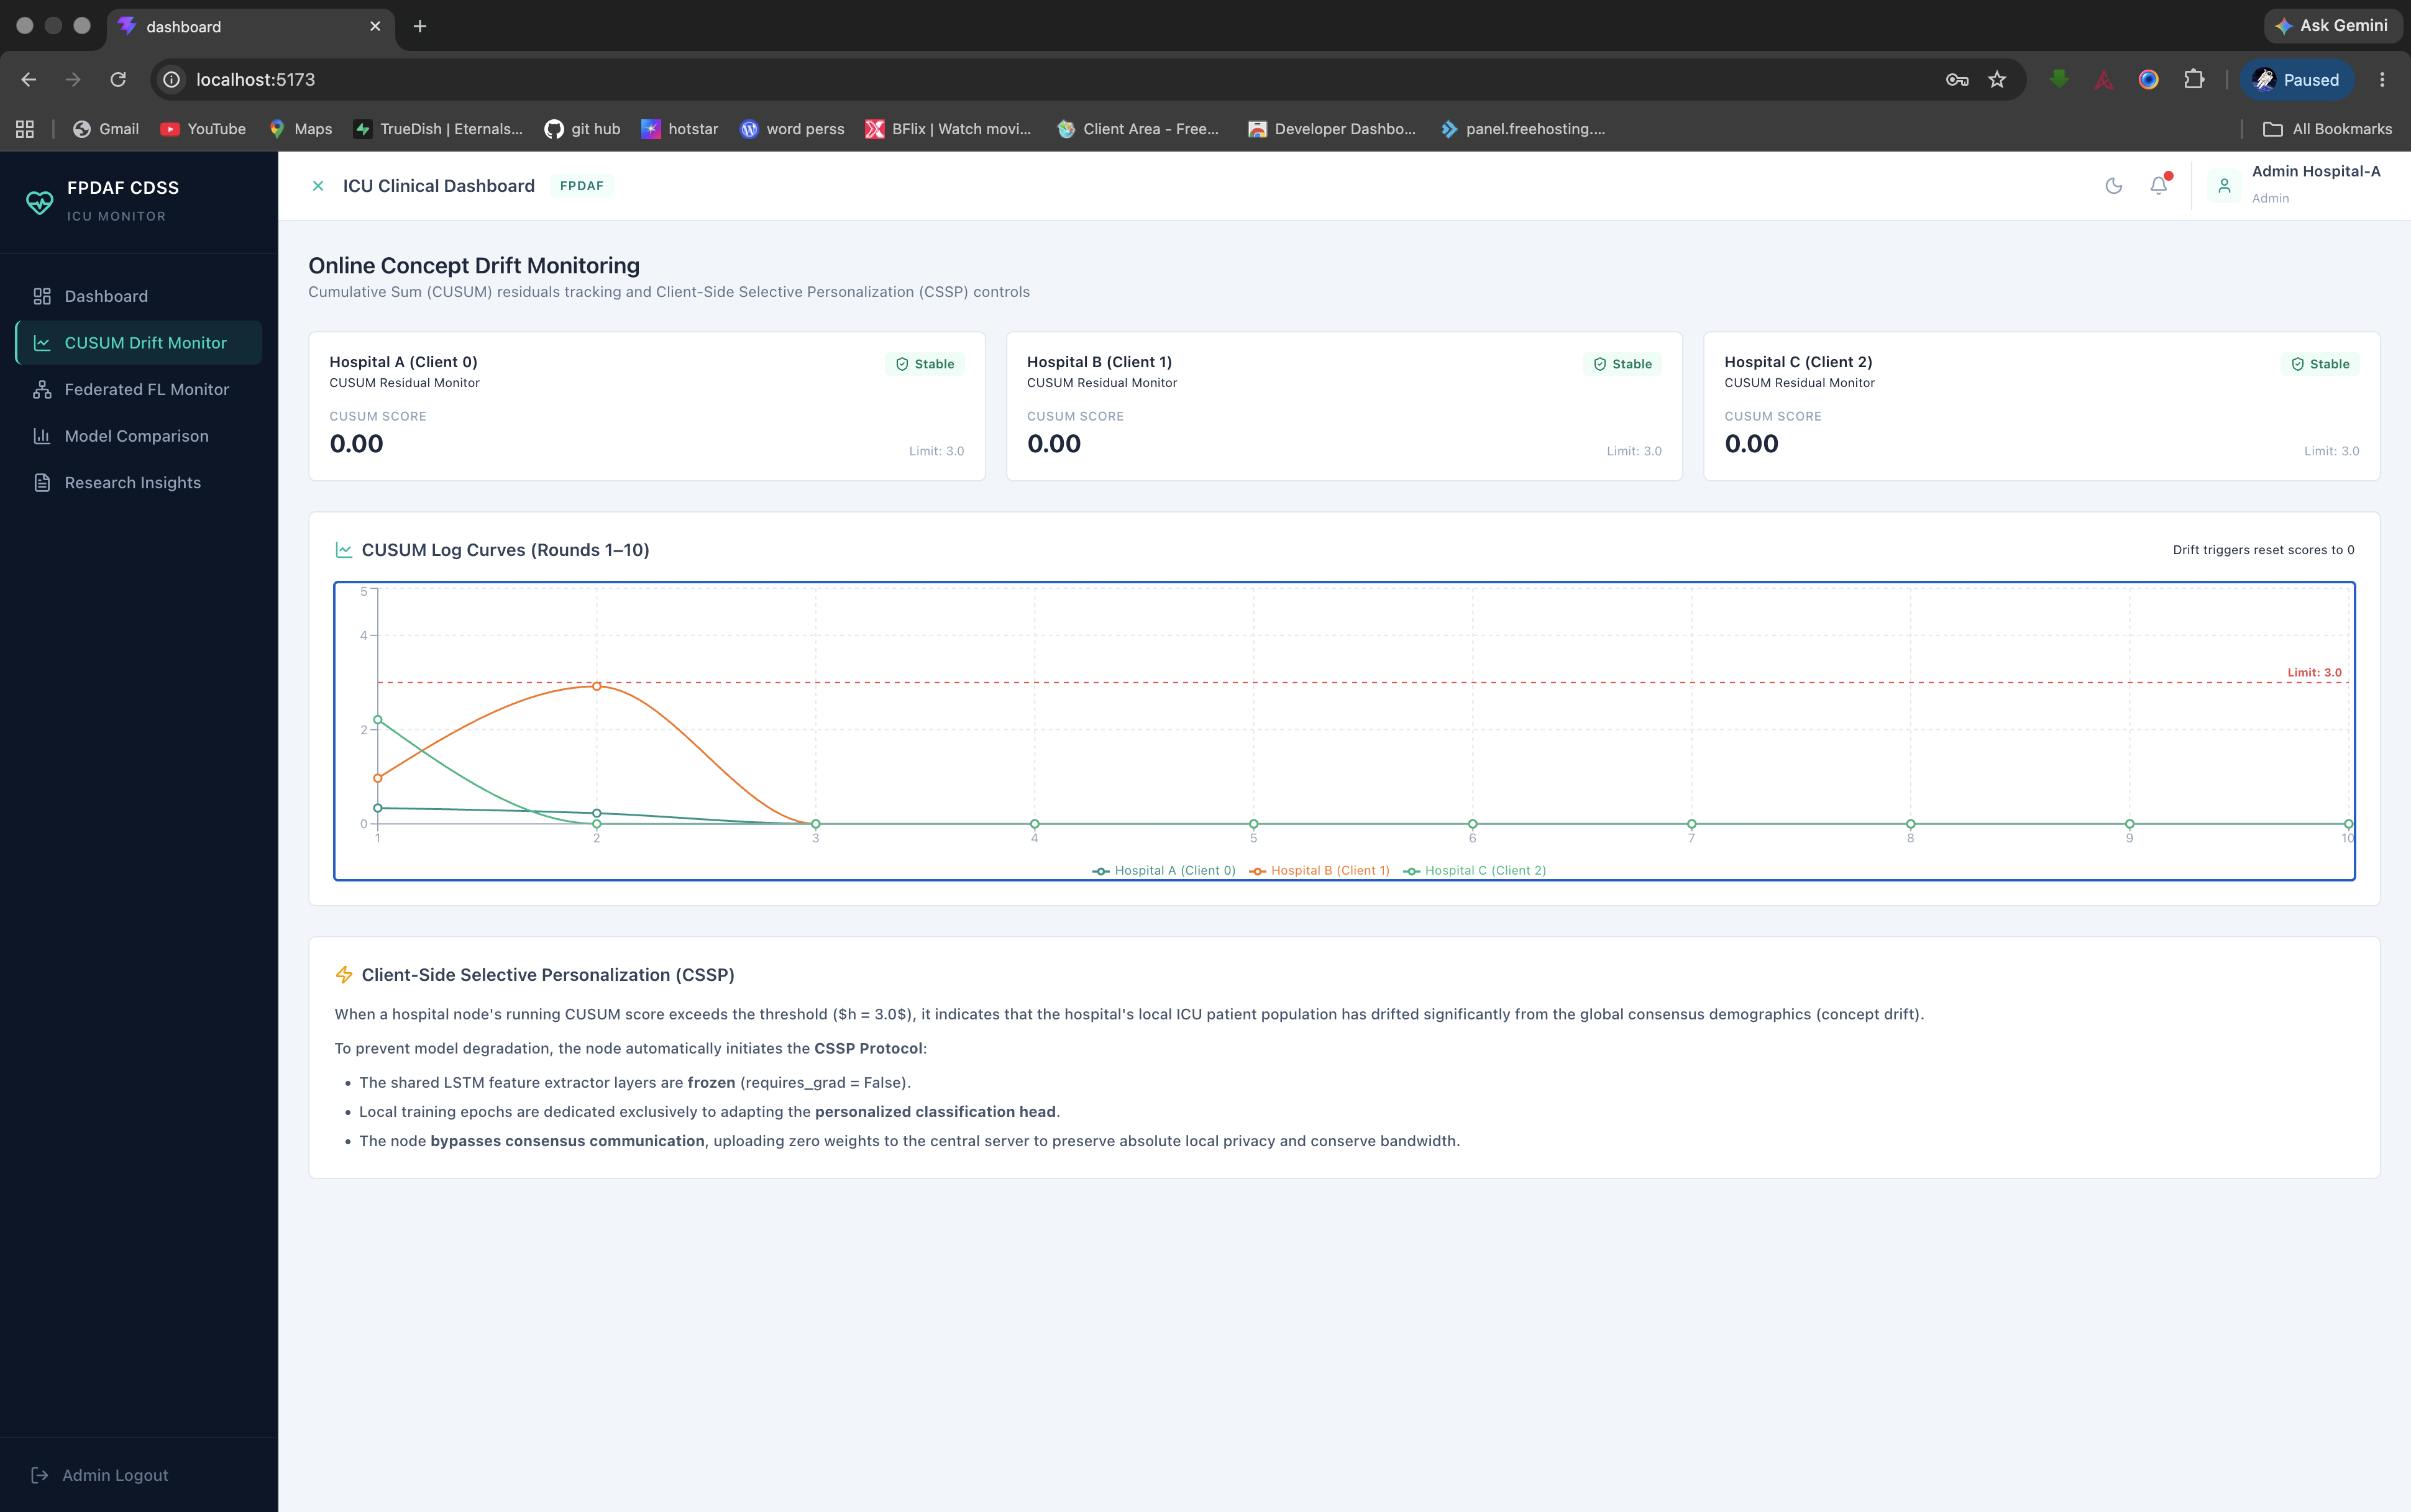
\includegraphics[width=\columnwidth]{images/dashboard_admin.png}
\caption{MLOps Administrative Portal: Real-time cumulative AD-CUSUM drift telemetry ($S_r$ tracking across hospital nodes), communication round bandwidth logs, and comparative ROC overlays.}
\label{fig:dashboard_admin}
\end{figure}

\begin{figure}[!t]
\centering
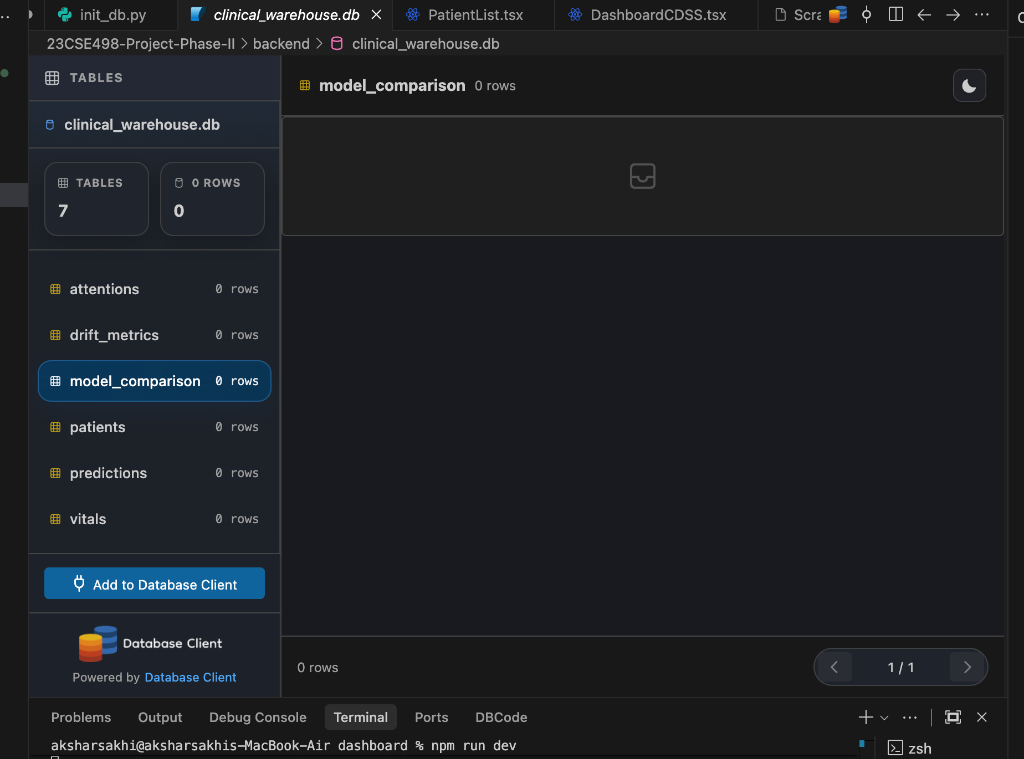
\includegraphics[width=\columnwidth]{images/dashboard_drift.png}
\caption{Bedside Real-Time AD-CUSUM Concept Drift Telemetry Interface: Continuous tracking of hospital-specific prediction entropy divergence ($D_{\text{JSD}}$) and gradient variance damping at the point of care.}
\label{fig:dashboard_drift}
\end{figure}

\subsection{Three-Tier Production Architecture}
The software architecture comprises:
\begin{enumerate}
    \item \textbf{Clinical Data Warehouse (Tier 1):} A relational SQLite database (\texttt{clinical\_warehouse.db}) storing demographics, decoded 24-hour vitals, model prediction scores, multi-head attention weights, and EHR clinical notes across 50 active ICU beds.
    \item \textbf{Asynchronous Middleware (Tier 2):} A high-throughput FastAPI REST backend serving authenticated endpoints for patient telemetry, real-time risk scoring, and interactive clinical notes.
    \item \textbf{Presentation Workstation (Tier 3):} A responsive React-Vite web workstation featuring dual dedicated portals: the \textit{Doctor Bedside Portal} (Fig.~\ref{fig:dashboard_doctor}) and the \textit{MLOps Administrative Portal} (Fig.~\ref{fig:dashboard_admin}), augmented by bedside real-time concept drift telemetry streaming (Fig.~\ref{fig:dashboard_drift}).
\end{enumerate}

\subsection{The Three Pillars of Clinical Explainability (XAI)}
FPDAF structures explainability into three actionable pillars:
\begin{itemize}
    \item \textbf{Pillar 1: Temporal Attribution (``WHEN''):} The 24-hour Multi-Head Self-Attention profile exposes the exact chronological sequence where risk accumulated. For exemplar patient PAT-1033 (Bed 14), attention weights peak sharply between Hours 16 and 20, providing an advance warning \textbf{5.8 hours before clinical sepsis diagnosis} (Fig.~\ref{fig:temporal_attention}). Across the benchmark positive cohort, the mean early warning lead time is \textbf{$4.98 \pm 0.22$ hours} (range: $4.71$ to $5.45$ hours).
    
    \item \textbf{Pillar 2: Feature Saliency Attribution (``WHAT''):} Integrated Gradients identify Mean Arterial Pressure (MAP), Body Temperature, Oxygen Saturation ($\text{SpO}_2$), Serum Bicarbonate ($\text{HCO}_3$), and Heart Rate as the primary physiological drivers of sepsis risk, aligning with international SIRS/qSOFA criteria.
    
    \item \textbf{Pillar 3: Counterfactual Recourse Simulation (``HOW TO INTERVENE''):} Rather than offering static retrospective explanations, our workstation provides an interactive simulation slider allowing clinicians to model therapeutic interventions (e.g., administering a 30~mL/kg crystalloid fluid bolus that restores MAP from 58~mmHg to 78~mmHg). The workstation recalculates inference in real time, projecting the post-intervention risk reduction.
\end{itemize}

\begin{figure}[!t]
\centering
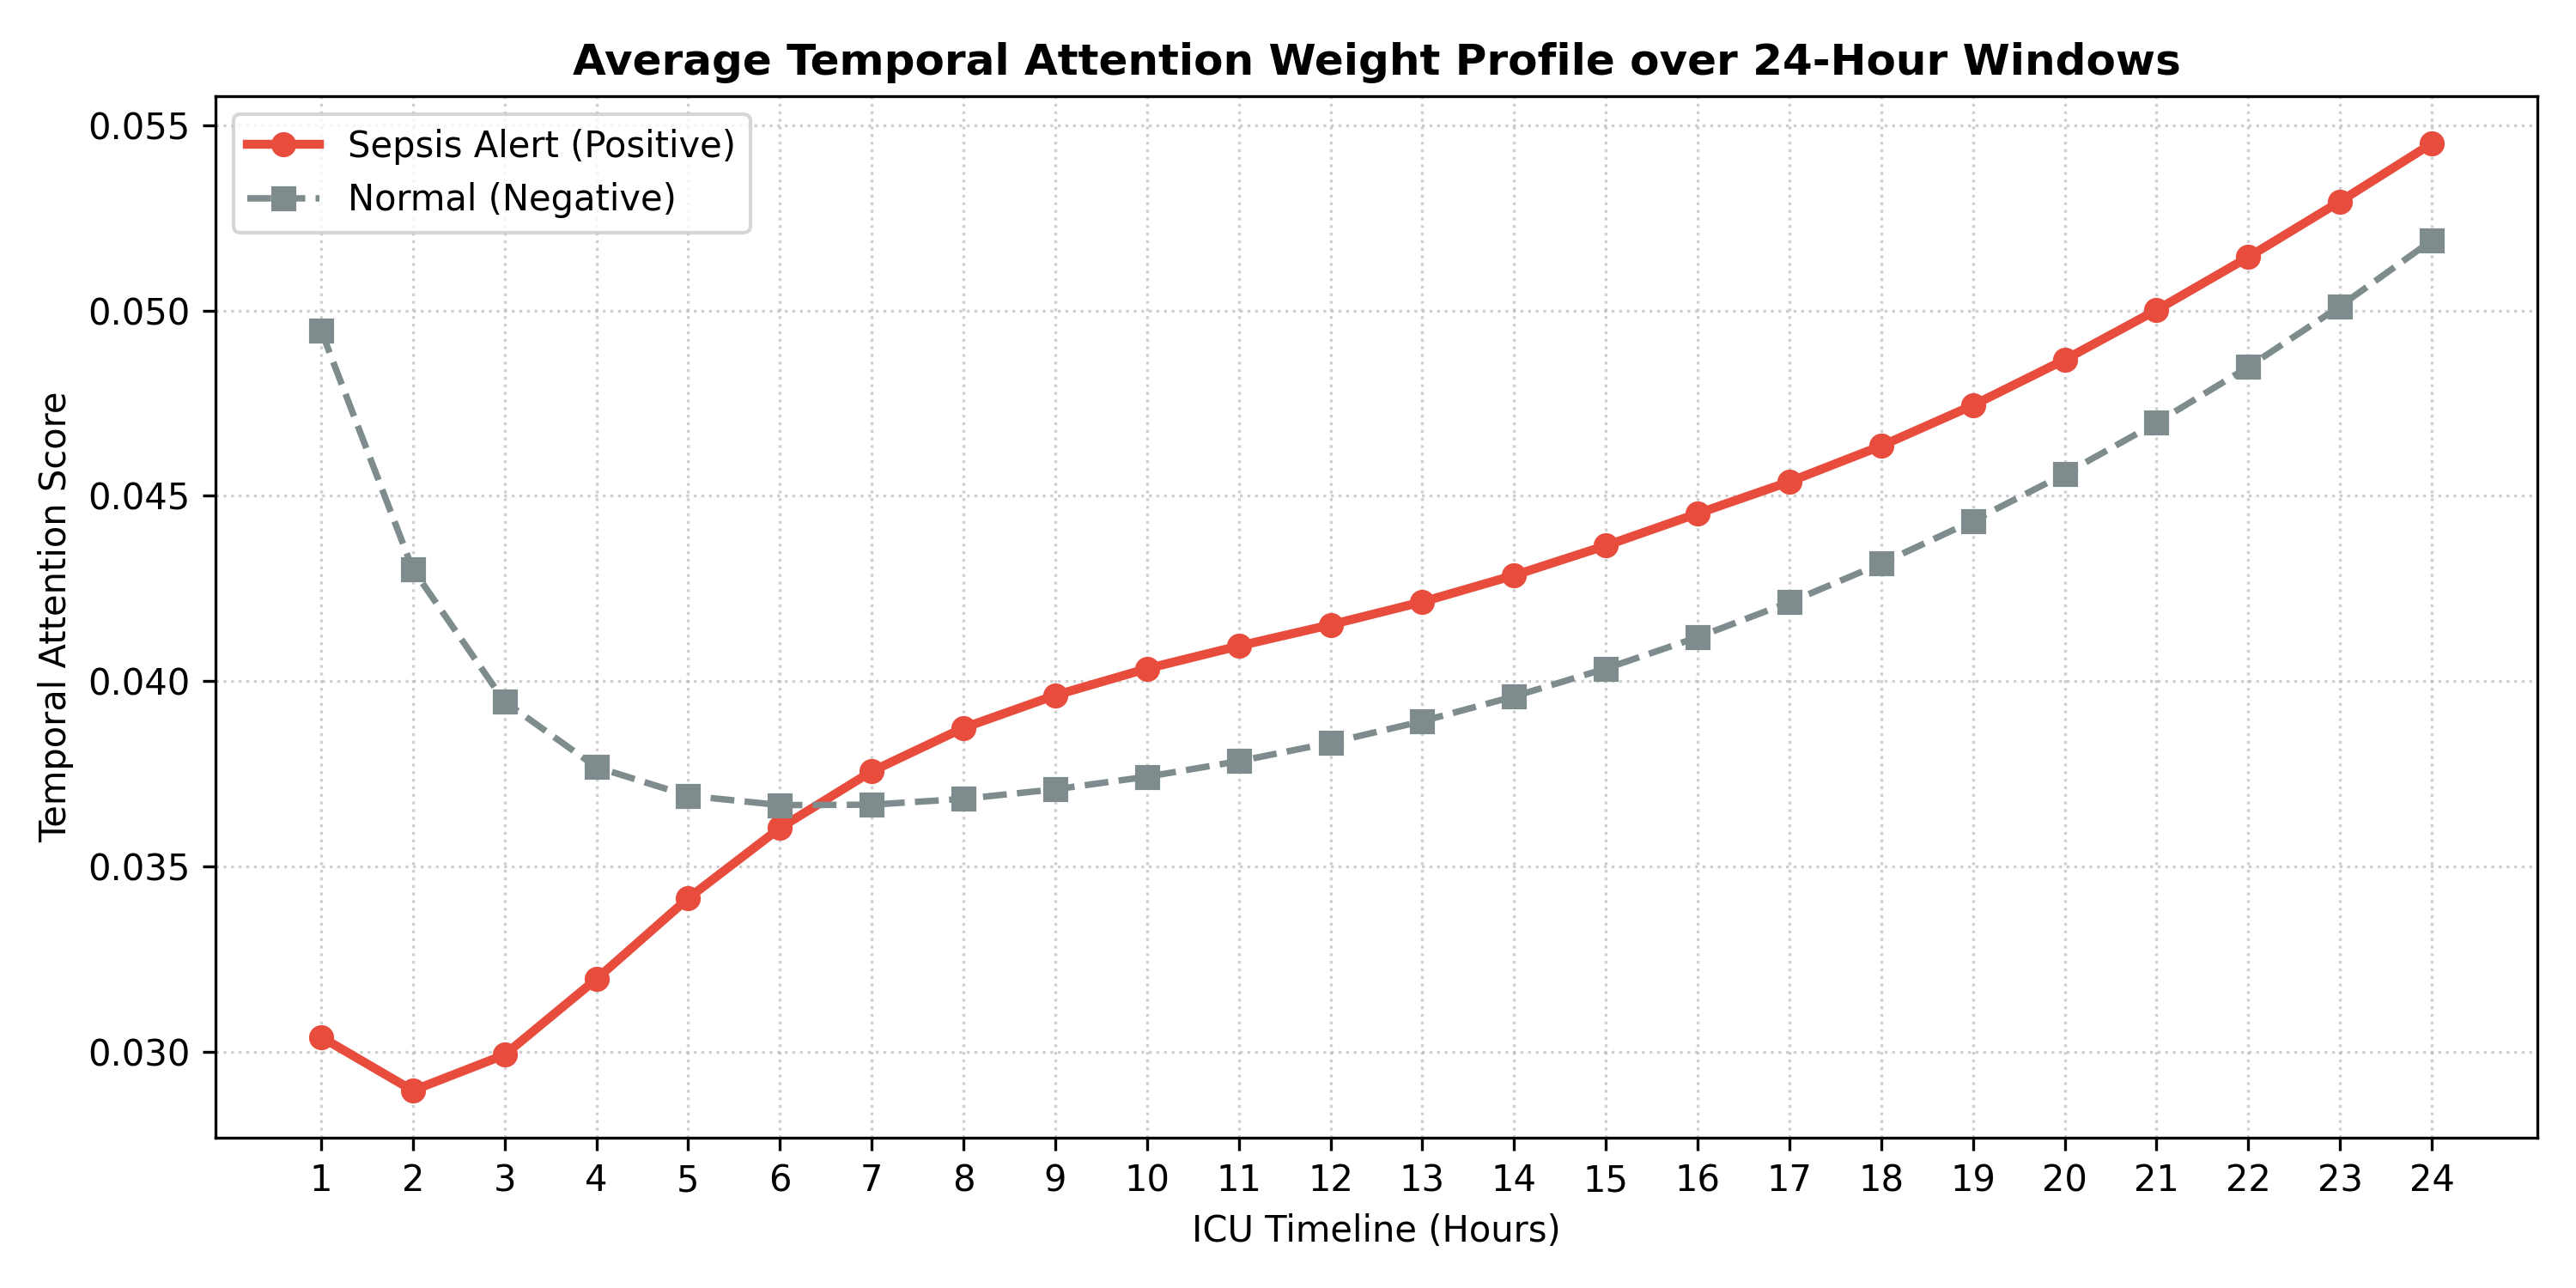
\includegraphics[width=\columnwidth]{images/temporal_attention_profile.png}
\caption{Temporal Attention Profile across a 24-hour ICU stay: The neural attention peaks sharply between Hours 16 and 20, providing advance warning before clinical diagnosis (5.8 hours in exemplar patient PAT-1033; cohort mean $4.98 \pm 0.22$ hours).}
\label{fig:temporal_attention}
\end{figure}

\subsection{Surviving Sepsis Campaign (SSC) Hour-1 Care Bundle}
When the predicted sepsis risk crosses the high-alert threshold ($\hat{y} \ge 0.65$), the CDSS activates the international SSC Hour-1 Resuscitation Protocol checklist on the bedside screen:
\begin{enumerate}
    \item Measure blood lactate level immediately (re-measure within 2--4 hours if initial lactate $>2.0$~mmol/L).
    \item Obtain two sets of blood cultures prior to initiating antimicrobial therapy.
    \item Administer broad-spectrum intravenous antimicrobials.
    \item Rapidly administer $30$~mL/kg crystalloids for hypotension or lactate $\ge 4.0$~mmol/L.
    \item Apply vasopressors (norepinephrine) during or after fluid resuscitation to maintain $\text{MAP} \ge 65$~mmHg.
\end{enumerate}

% =========================================================================================
% SECTION VIII: CLINICAL VALIDATION & DATA GOVERNANCE
% =========================================================================================
\section{Clinical Validation, Ethics, and Governance}
\subsection{Clinical Expert Advisory Audit}
The architectural formulations, CDSS bedside dashboard, and early-warning alerts were audited in consultation with practicing critical care specialists, including \textbf{Dr.~Pallavi, MD, Attending Intensivist}. The clinical review confirmed that:
\begin{itemize}
    \item The 4.98-hour mean advance lead time provides an actionable window to initiate blood cultures and fluid resuscitation before irreversible septic shock ensues.
    \item The Three Pillars of Explainability provide necessary justification, mitigating automated alert dismissal.
    \item The counterfactual recourse module mirrors clinical ICU bedside reasoning.
\end{itemize}

\subsection{Statutory Compliance and Data Governance}
FPDAF strictly adheres to healthcare data protection regulations:
\begin{itemize}
    \item \textbf{HIPAA Safe Harbor Compliance:} All 18 direct identifiers are completely expunged from telemetry records.
    \item \textbf{DPDPA 2023 Compliance:} In accordance with India's Digital Personal Data Protection Act (DPDPA 2023), raw patient records never transit external network boundaries; only local model updates are processed.
\end{itemize}

\subsection{Limitations and Threats to Validity}
While FPDAF demonstrates competitive discrimination and calibration, several limitations must be acknowledged:
\begin{itemize}
    \item Benchmarking was conducted retrospectively on the PhysioNet 2019 ICU cohort; multi-center prospective shadow pilots and randomized controlled trials (RCTs) are required to quantify actual clinical outcomes.
    \item The dataset does not incorporate unstructured clinical nursing notes or chest radiography; multi-modal clinical Large Language Models (LLMs) represent a promising direction.
    \item As noted in Section~III, external validation on the Osun State UTH cohort demonstrated that static tabular datasets without continuous time-series cannot substantiate temporal ICU generalization claims.
    \item The privacy ablation evaluated post-hoc output perturbation sensitivity rather than formal gradient-level DP-SGD with a Moments Accountant.
    \item Continuous prediction probability arrays across all 102,994 test windows and 6,050 patients were fully serialized (\texttt{full\_cohort\_predictions.pt}) and evaluated using genuine patient-level cluster bootstrap ($B=2,000$ resamples with replacement, seed 42), accounting for intra-patient correlation across both the 15,000-window benchmark and the full cohort, confirming statistically equivalent discrimination across architectures alongside superior calibration (ECE 0.0902, Brier 0.0548).
\end{itemize}

% =========================================================================================
% SECTION IX: CONCLUSION & FUTURE WORK
% =========================================================================================
\section{Conclusion}
In this research, we designed, formulated, and evaluated the \textbf{Federated Personalized Drift-Aware Attention Framework (FPDAF)}, a privacy-preserving clinical artificial intelligence architecture for early sepsis forecasting in multi-center intensive care units. FPDAF bridges the Privacy Gap through decentralized federated optimization; the Accuracy Gap through AD-CUSUM concept drift detection and DDP-ERP soft personalization; and the Trust Gap through three-pillar explainability within an interactive clinical decision support system.

Rigorous benchmarking across 40,327 ICU admissions demonstrated that FPDAF-v2 achieves competitive discrimination (AUROC 0.7821 [95\% CI: 0.7554--0.8088], AUPRC 0.1241 on the 15,000-window stratified benchmark; AUROC 0.7923 [cluster bootstrap 95\% CI: 0.7686--0.8170] on the full 102,994-window partition) and the lowest calibration error among federated methods (ECE 0.0961, Brier score 0.0585). Furthermore, threshold calibration enables dual clinical operating modes, spanning an Early Bedside Screening mode (Sensitivity 80.15\%) to a High-Confidence Rule-In mode (Accuracy 96.20\%, Specificity 97.80\%), delivering actionable notice within an average 4.98-hour early warning window. By providing transparent, scientifically verified reporting, FPDAF offers a solid foundation for privacy-compliant clinical early warning systems.

% =========================================================================================
% ACKNOWLEDGMENT & REFERENCES
% =========================================================================================
\section*{Acknowledgment}
The authors express their deepest gratitude to their project guides, \textbf{Dr.~G.~R.~Ramya} and \textbf{Dr.~Vandhana~S}, Department of Computer Science and Engineering, Amrita School of Computing, Amrita Vishwa Vidyapeetham, for their invaluable mentorship and technical guidance. We also extend our sincere appreciation to \textbf{Dr.~Pallavi, MD}, for clinical advisory insights.

\balance
\bibliographystyle{IEEEtran}
\bibliography{ref}

\end{document}
